\documentclass[twocolumn]{article}
\usepackage[left=2cm,right=2cm,top=2cm,bottom=2cm]{geometry}
\usepackage[utf8]{inputenc}
\usepackage{graphicx}
\usepackage{tabularx}
\usepackage{url}
\usepackage{multicol}
\usepackage{layout}
\usepackage{xcolor}
\usepackage{listings}



\lstdefinestyle{custompython}{
    language=Python,                    % 设置语言
    basicstyle=\ttfamily\footnotesize,  % 设置代码字体为等宽字体,且字号为脚注大小
    keywordstyle=\bfseries\color{blue}, % 设置关键字的样式
    commentstyle=\itshape\color{gray},  % 设置注释的样式
    stringstyle=\color{orange},         % 设置字符串的样式
    numbers=left,                       % 在代码左侧显示行号
    numberstyle=\tiny\color{gray},      % 设置行号的样式
    stepnumber=1,                       % 每一行都显示行号
    numbersep=10pt,                     % 行号和代码之间的距离
    showstringspaces=false,             % 不显示字符串中的空格
    breaklines=true,                    % 代码过长时自动换行
    backgroundcolor=\color{gray!10},    % 代码的背景颜色
    breakatwhitespace=true,             % 只在空格处换行
    tabsize=4,                          % 设置 Tab 的宽度
    captionpos=b                        % 设置标题的位置为底部
}

\lstset{style=custompython}
\setlength{\columnsep}{0.2in}
\graphicspath{{images/}}


\begin{document}

\begin{titlepage}
    \begin{center}
        \begin{figure}[h]
            \centering
            
\includegraphics[scale = 0.15]{liverpool logo.png}
        \end{figure}
        \textsc{\\[2.5cm]\Huge COMP390 Project Dissertation\\[0.5cm]}
        \textsc{\LARGE 2023/24\\[2cm]}
        \textsc{\huge Project Name: MCQ Scanner\\[1cm]}
        \textsc{\Large Hailin Xie (ID:201677247)\\[0.5cm]}
        \textsc{\Large Supervisor: Dr. D. Wojtczak\\[0.5cm]}
        \textsc{\Large {\today}\\[6cm]}
        \textsc{\Large Department of Computer Science\\[0.5cm]}
        \textsc{\Large University of Liverpool\\[0.5cm]}
        \textsc{\Large Liverpool L69 3BX\\[0.5cm]}

    \end{center}
\end{titlepage}

\section*{Acknowledgements}
    % \begin{multicols}{2}    
        \noindent

        This project dissertation is dedicated to my family, friends, and mentors, whose unwavering support and encouragement have been the driving force behind my academic pursuits. Their belief in my potential and their guidance have been the foundation upon which I have built my academic career. 

        I would like to extend my deepest gratitude to my parents, whose unwavering support and encouragement have been indispensable throughout my undergraduate journey.

        I must express my heartfelt thanks to my mother, Hui. Her boundless love, understanding, and sacrifices have not only eased my academic endeavors but have also been a source of strength in times of challenge. Her presence and support in every aspect of my life have been a constant reminder of what true dedication looks like.
        
        Equally, I owe a profound debt of gratitude to my father, Bing. It was he who first introduced me to the fascinating world of computer science. His guidance and teachings were the first steps that set me on this path, igniting a passion for the field that has only grown stronger with time. His wisdom and patience have been my guiding lights, helping me navigate both my studies and my personal growth. Their combined efforts have provided me with the foundation upon which I have built my academic career. Their examples of perseverance and commitment have taught me invaluable lessons that extend beyond the classroom. It is because of their love and belief in my potential that I have been able to pursue my dreams with confidence.

        Grandfather Chenghai has been a cornerstone of my life, offering not just support but also teaching me the values of integrity and resilience. His lessons on how to conduct oneself in life, with a steadfast heart and unyielding purpose, have been invaluable. He instilled in me the importance of never losing sight of one's origins and principles, no matter the achievements or the altitude one reaches. This foundational philosophy has been my guiding star, influencing every decision and ambition I have pursued.

        I dedicate this and to the memory of my paternal grandfather, Changgui, whose memory I cherish with every success. He's belief in the power of education and his dream of seeing me flourish academically took me across borders to study in a foreign country. The spirit and hopes for me have remained a constant source of motivation, his legacy lives on in my pursuit of knowledge and my commitment to excellence. I am forever grateful for his unwavering support and love. 

        I am deeply grateful to my friends Zhaoxin and Xiaoqiao, whose companionship has been a beacon of support and warmth during my time abroad. Despite the physical distances that separate us, their presence has been a constant reminder that I am never truly alone. Zhaoxin's unwavering encouragement and Xiaoqiao's heartfelt conversations have transformed my experience in a foreign land into one filled with cherished moments and laughter. Their ability to bring joy into everyday interactions and to provide a sense of home away from home has been invaluable. I am fortunate to have friends who not only understand the challenges of living abroad but who also go out of their way to ensure that these challenges are met with shared strength and optimism.
        
        I would also like to extend my deepest gratitude to my friends and project members, Chenwei, Zekai, Tianyao, and Zijian, for their invaluable contributions to this project. Their tireless efforts in creating the dataset crucial for training our machine learning algorithm were instrumental to the timely completion of our project. Their selfless dedication not only provided the essential data needed but also their technical support throughout the project significantly accelerated our progress.

        Special thanks are also owed to my good friend Gubin, who provided substantial technical support during the early stages of this project. His insights and partial contributions to the original code of our algorithm were not only inspirational but pivotal to the foundational aspects of our work. I am profoundly grateful for his enthusiastic and generous assistance.
        
        Without the collective efforts, support, and expertise of Chenwei, Zekai, Tianyao, Zijian, and Gubin, this project could not have reached its successful fruition. I am immensely thankful for their camaraderie and expert collaboration. Their unwavering commitment to our shared goals and their dedication to the project have been a source of inspiration and motivation. I am fortunate to have had the opportunity to work alongside such talented and driven individuals, whose combined efforts have been instrumental in the completion of this project.

        I would like to express my gratitude to my supervisor, Dr. D. Wojtczak, whose guidance and support have been instrumental in the completion of this project. His expertise and insights have been invaluable, providing me with the tools and knowledge necessary to navigate the complexities of this research. I am deeply grateful for his unwavering support throughout this project.

        Finally, I would like to thank the Department of Computer Science at the University of Liverpool for providing me with the opportunity to pursue my academic interests. The resources and support offered by the department have been invaluable, enabling me to explore my passion for computer science and to develop my skills in this field. The academic environment at the University has been conducive to learning and growth, fostering an atmosphere of collaboration and innovation. I am grateful for the opportunities and experiences that the department has provided me.

\hspace*{\fill}

        -- \textbf{Hailin Xie, 2024/5/9 at Liverpool, UK}
        
    % \end{multicols}



\newpage
\begin{titlepage}
    \begin{center}
        \begin{figure}[h]
            \centering
            
\includegraphics[scale = 0.15]{liverpool logo.png}
        \end{figure}
        \textsc{\\[2.5cm]\Huge COMP390 Project Dissertation\\[0.5cm]}
        \textsc{\LARGE 2023/24\\[2cm]}
        \textsc{\huge Project Name: MCQ Scanner\\[1cm]}
        \textsc{\Large {\today}\\[8cm]}
        \textsc{\Large Department of Computer Science\\[0.5cm]}
        \textsc{\Large University of Liverpool\\[0.5cm]}
        \textsc{\Large Liverpool L69 3BX\\[0.5cm]}

    \end{center}
\end{titlepage}
\onecolumn
\begin{center}
    \textsc{\\[2cm]\Large Statement of Ethical Compliance\\[2cm]}
\end{center}


    \textbf{Data Catecory:A}

    \textbf{Participant Category:0}
    


    The data and participant categories for this project is A-0 (No use of data derived from humans or animals - No use of human participants in any activity).All datasets (test set, training set) used in this project are virtual data created by the project supervisor and researchers themselves to simulate real situations. The content of datasets does not originate from any public or non-public APIs, and does not constitute a breach of privacy for any person. I solemnly confirm that I will follow the Ethical Guidance of COMP390 Honours Year Project.

\vspace{2cm}
\begin{abstract}
    % \begin{multicols}{2}
        \noindent
        During the annual semester exam week, the academic affairs departments of educational faculties need to handle a large number of final exam papers from various colleges, especially machine readable answer sheets. However, answer sheets that require specialized equipment to process often take several weeks to be fully scanned, putting a significant workload on faculty and staff. Therefore, developing an application that can partially replace specialized scanners and allow individuals to process answer sheets is of practical significance.

        This dessertation presents the development of an innovative web-based application designed to automate the recognition and processing of scanned multiple-choice question (MCQ) answer sheets based on optical mark recognition(OMR) technology. Utilizing advanced machine learning algorithms, the application identifies both student details and their answers from scanned sheets, subsequently automating the grading process and generating detailed score reports. Furthermore, MCQ-Scanner supports the generation of statistical analyses and the automated dispatch of feedback emails to students, enhancing the educational feedback loop. 
        
        The primary aim of this project is to obviate the need for specialized scanning hardware traditionally required for MCQ assessments, thereby saving time for educational institution staff. Developed exclusively for use with the University of Liverpool's answer sheets, the application leverages Python, PyTorch, and OpenCV for backend processes, with a front-end built using Node.js, CSS, and HTML, and server management via Python Flask. 
        
        A bespoke dataset was crafted for training the machine learning model, which after extensive testing and refinement, demonstrated optimal performance using a pretrained Wide ResNet model for both option recognition and student identification, achieving accuracy rates exceeding 99\% and a processing time of approximately 0.4 seconds per sheet. This tool represents a significant advancement in the digitalization and automation of educational assessment processes.  

        
    % \end{multicols}
\end{abstract}

\begin{center}
    \textbf{Keywords: Machine learning, Grading, Image processing, Optical mark recognition, Python, OpenCV}
\end{center}


\newpage
\tableofcontents
\newpage

% \begin{multicols}{2}
\twocolumn
\section{Introduction and Background}
    \subsection{Introduction}
        An optical answer sheet or bubble sheet is a special type of form used in multiple choice question (MCQ) examinations. The sheet is printed with black bars (anchor points), allowing the scanner to confirm the direction and position of the sheet\cite{OMR_def}. Optical Mark Recognition (OMR) technology is commonly used to automate the processing of these answer sheets.The infrared radiation emitted by answer sheet readers (usually improved scanners) is sensitive to carbon in pencil marks. By measuring the transmittance of different parts of the answer sheet, the scanner can obtain answers on the paper\cite{OMR_wiki}. In normal situations, education and government agencies possess a large number of such expensive scanners. But for individuals, it would be neither difficult to process these answer sheets in bulk, Nor can teachers quickly obtain students' grades. At the same time, traditional scanners are also prone to errors when facing situations where the answer sheet is stained, bent, and the answer handwriting is not clear enough. \textbf{Therefore, the goal of this project is to develop a web-based program that allows users to upload scanned files of MCQ answer sheets and identify their content.} Machine learning (ML) and computer vision (CV) is used to identify the answers filled in the answer sheet and compare them with the correct answer template uploaded by the user to obtain the results of each test paper. Users can then view and download transcripts on the webpage. The website also supports automatic sending of emails to exam participants, notifying them of their exam results.

        \begin{figure}[h]
            \centering
            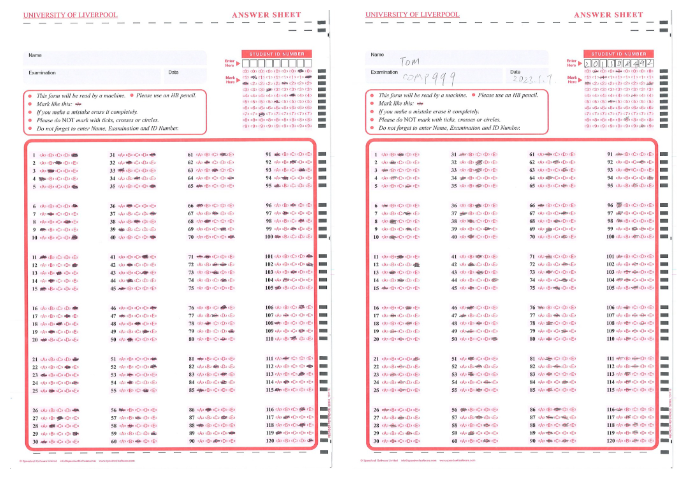
\includegraphics[width=0.3\textwidth]{ans_sheet.png}
            \caption{An example of MCQ answer sheets.}
            \label{fig:ans_sheet}
        \end{figure}

        The optical mark recognition technology based on OpenCV has been widely used in the field of answer sheet recognition. In fact, some scanners specifically designed for scanning answer sheets have similar built-in  software. However, it should be noticed that few attempts has been made to associate this algorithm with machine learning models. These programs merely using OpenCV for recognition is beneficial, since they require less computing resources. This of vital importance for websites deployed on servers. However, due to these programs often rely solely on a fixed set of logic to identify answers, they are very unstable when facing interference, and program design based solely on OpenCV cannot provide corresponding solutions. Therefore, this project aims to use machine learning models to assist in the recognition of answer sheets. The model can be trained on a large number of answer sheets to improve the accuracy of recognition. In addition, the machine learning model can also be used to identify the student's name and student number on the answer sheet, which is very important for the subsequent grading process.
       
    \subsection{Background}
        The objective of this work was to develop Optical Mark Recognition (OMR) software for implementation on network and for its usage as an OMR machine. \textbf{A key point of this project is the ability to identify non-standard answers. }This means that the model needs to identify pencil marks that have not been filled "correctly" according to the requirements and guidelines at the beginning of the answer sheet. Generally speaking, a standard filling case is to completely cover the letters on the answer sheet with pencil marks, resulting in a black block of notes. However, some students only draw a horizontal line on the letters or use pencils to make other markings on the letters, which undoubtedly poses a great challenge to the accuracy of the model\cite{OCR_1}. In the fields of OMR and OCR, in order to better extract image features, various pre-processing methods are usually used to enhance the features that need to be extracted. Adrian Roserock\cite{CV_1} mentioned four steps required to process such scanned images or photos using OpenCV\cite{opencv}:

        \begin{itemize}
            \item Read the image and convert it into a grayscale image, while obtaining the target question.The usual approach is to cut single question images based on coordinates.
            \item Perform grayscale, binarization, and corrosion operations on the target image. The focus of this step is to perform morphological processing on the image to reduce the processing load of image data for subsequent contour retrieval. The binary operation often uses the OTSU algorithm\cite{OTSU}.
            \item Edge detection, finding contours, drawing contours. This step is to find the contour area of the image. When calling the contour function, only the outer contour is usually obtained, with a parameter value. The edge detection method usually uses the Canny algorithm\cite{canny}, which can be replaced with other algorithms.
            \item Determine user answers through the x-coordinate of the bounding rectangle. This step requires relying on an answer dictionary for user answer judgment, which is defined  where the key values of the dictionary are (options, corresponding x coordinate range). The values in this dictionary are adjusted based on the format and content of the answer sheet\cite{canny_wiki}.
        \end{itemize}

        This process demonstrates how a regular answer sheet scanner processes input images. A main feature of this method is that it cuts the input image and divides the answer sheet into different regions for recognition. This can significantly improve the accuracy of recognition\cite{Meesad}, and generally has good processing results for simple answer sheets. Benedito et al.\cite{Optical} used the GEXCAT software package to automatically read multiple choice questions and were able to accept PDF and latex files.However, Viraj Jain\cite{OMR_ieee1} mentioned that \textbf{this method can only achieve high recognition accuracy for structurally simple answer sheets} (with obvious features, such as SAT exam answer sheets, the bubbles are large and obvious). For this reason, \textbf{ neural network models are used for image recognition, rather than simply detecting filling marks in the image.} The neural network model is very suitable for processing complex images, and it is hoped that training can improve the recognition accuracy of non-standard filling styles in a targeted manner.


        \begin{figure}[h]
            \centering
            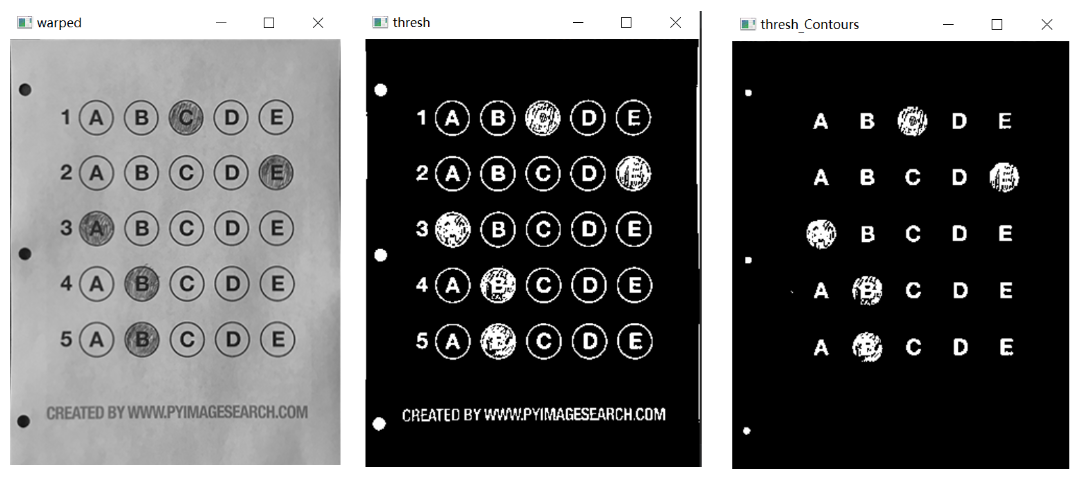
\includegraphics[width=0.4\textwidth]{opencv_omr.png}
            \caption{An example using OpenCV to recognise answers on a MCQ answer sheet\cite{OpenCV_sheet}.}
            \label{fig:opencv_omr}
        \end{figure}


        Among numerous improvement schemes, the introduction of convolutional neural network(CNN)\cite{cnn_1}  models seems to be an effective solution. Wang et al.\cite{omr_ieee2_wang} used deep learning tools in TensorFlow to construct CNN models for mark recognition. In the experiment, they constructed a CNN model consisting of two convolutional layers, two pooling layers, and two fully linked layers. They preprocess OMR input data through TensorFlow to obtain TFRecord files, and then train the model to achieve the required OMR recognition level in the test set and obtain standard parameters. Sarika et al.\cite{omr_ieee3} used the CNN model based on VGG-16 architecture to classify and recognize target symbols (circles, blocks) in low light environments. Intersecting with ordinary OMR detection, the recognition accuracy of the CNN model can reach 99.9\%.By comparison, Agarwal et al.\cite{Scanner} achieved an accuracy of only 97.6\% using multiple computer vision algorithms for recognition.

        In the early stages of project development, this project was committed to adaptating for low performance devices. \textbf{Therefore, the selection of models becomes crucial. In the expected usage scenario of this project, users often need to continuously scan hundreds of answer sheets, and the project will run on the server with no GPU acceleration avaliable, so the computational resources need to be minimized.} In normal CNN models such as Xception and ResNeXt\cite{ResNeXt}, the presence of a large number of dense $1 * 1$ convolutions made the network very inefficient\cite{Zeki}, so the preliminary task of this project is to train a sufficiently simple and accurate neural network model that meets the requirements.

        In 2017, Zhang et al.\cite{zhang2017shufflenet} proposed using pointwise group convolutions to reduce the computational complexity of 1 * 1 convolution, while also proposing channel shuffles to assist in the flow of information in different feature channels. In order to make good use of channel shuffle operations, the author proposes the ShuffleNet model. ShuffleNet is designed to reduce computational complexity and parameter count while maintaining good performance for efficient operation in resource constrained environments.


        \begin{figure}[h]
            \centering
            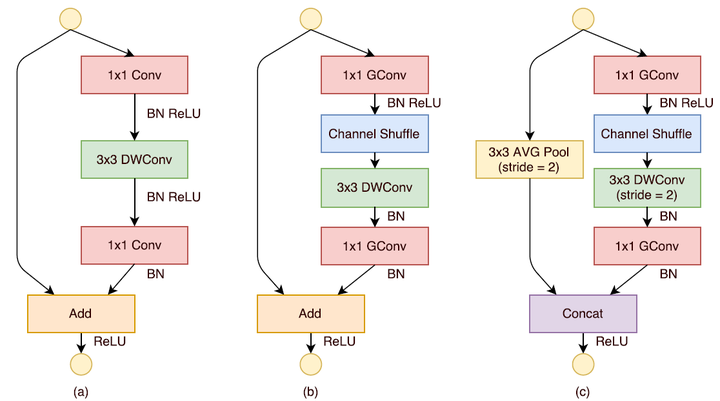
\includegraphics[width=0.4\textwidth]{shuffle_net.png}
            \caption{The architecture of ShuffleNet.}
            \label{shuffle_net}
        \end{figure}

        The key features of ShuffleNet include\cite{zhang2017shufflenet}:

        \begin{itemize}
        \item \textbf{Group convolution:} ShuffleNet uses group convolution to divide the input feature map into multiple groups, and each group undergoes convolution operations. This helps to reduce the number of parameters and computational burden.
        \item \textbf{Channel shuffling:} ShuffleNet introduces channel shuffling operations, which rearrange information between channels to increase the transmission and communication of information in the network. Channel shuffling helps improve the network's representation ability.
        \item \textbf{Bottleneck structure:} ShuffleNet uses a bottleneck structure, which includes a combination of 1x1 convolution, 3x3 deep separable convolution, and 1x1 convolution. This structure reduces the computational burden while maintaining the effectiveness of the network.
        \item \textbf{Multi scale feature fusion:} ShuffleNet also supports multi-scale feature fusion, allowing the network to better handle objects or objects of different sizes\cite{shufflenet2}.
        \end{itemize}

        The lightweight design of ShuffleNet\cite{MOUSSA1991283} makes it very suitable for this project. Meanwhile, considering that other related studies have also achieved good classification results using models of other architectures(Such as VGG, AlexNet, etc.), this project used multiple neural network architectures for comparison, and finally used Wide ResNet as the main model architecture. These details will be included in subsequent chapters.
        

\section{Aims and Requirements}
This section will mainly focus on the functions and detailed technical indicators that the software needs to implement. The specific items are as follows: 
    \subsection{Aims}
    \begin{itemize}
    \item \textbf{Image upload and pre-processing}: Create a webpage that allows users to upload answer sheets and standard answer templates in PDF format, the webpage needs to process these images (e.g, denoising, cropping, and enhancement) to extract answers and return the score of the answer sheet.
    \item \textbf{Feature extraction:} Using computer vision algorithms to extract the features of answers from answer sheet images, such as the position of multiple-choice questions, text recognition, etc.
    \item \textbf{Answer recognition:} Create a machine learning model that can accurately recognise and record the candidate's name, student ID and valid answers on the answer sheet.
    \item \textbf{Automatic grading:} Compare the scanned answer sheet with the standard answer template (CSV or PDF format) uploaded by the user to obtain the score of the answer sheet.
    \item \textbf{Visual feedback:} Provide users with visual feedback, showing which questions were answered correctly and which were answered incorrectly, and provide a detailed score report through interactive webpage elements.The results of analysis can be downloaded and sent to the candidate's email address.
    \end{itemize}

    \subsection{Requirements}
    \begin{itemize}
    \item\textbf{Upload Webpage (Homepage):} Create a webpage that allows users to upload answer sheets and standard answer templates separately. 
    \begin{itemize}
        \item The answer sheet should be in PDF format, and the standard answer template should also be in the same format or allow users to manually input answers (CSV format). Master solution given as a standard answer sheet or CSV file, with a seperate portal to upload.
        \item The standard answers uploaded in PDF format will be automatically analyzed and downloaded to the user's computer for viewing and modification.
        \item After uploading files, users can preview files on the webpage. If the uploaded files are incorrect, they can perform operations such as deleting or re-uploading them.
    \end{itemize}
    \item \textbf{Analysis Webpage:} Create a result analysis webpage that:
    \begin{itemize}
        \item Return a CSV (comma separated values) file with student ID, mark(out of 100, .5 rounded up), number of correct answers.
        \item Answers should be a string with the answers given by the student to each equation, if the answer is in capitial letter, then it is the correct answer,if the answer is in small letter then it is wrong. If the answer is "-", then it is not answered.
        \item Displays candidate's name, accuracy, student ID and the overall score of the answer sheet compared with the standard answer template.
        \item Calculate weights, some questions are worth more than others, this would be specified in the CSV.
        \item Users can set up parts of the test paper to distinguish between different areas of the test, and the program can provide scores for different parts separately, making it convenient for users to view.
        \item Automatically identify the total number of questions. MCQ question answering sheets often do not use up all the questions.
        \item If there are multiple candidates, the webpage will display the overall information of their grades, such as average score, median, highest and lowest scores, etc.
        \item Rank the questions based on overall accuracy and display them on the page.
        \item Send feedback and emails to candidates. Users can configure an SMTP email server in the source code and upload personal information of students on the website. The program will match student information with transcripts and send emails.
    \end{itemize}
    \item \textbf{Image processing:} Code an image processing function to preprocess the files uploaded by users:
    \begin{itemize}
        \item Read the scanned (both colored/black and white are supported) pdf files and convert it into images. Multiple pdf input files can be processed at the same time.
        \item Enhance the image quality, remove noise, and adjust the brightness and contrast of the image.
        \item Image segmentation, extract the answer area, and ignore the irrelevant area.
        \item Expanding corrosion or performing morphological operations to highlight the marked area.
        \item Edge detection and contour finding.
        \item Obtain the bounding rectangle to obtain the contour coordinates, set these points as anchor points.
        \item Deskew the image. Correct the image based on the obtained rectangular contour, including ignoring bends, correcting paper angles, etc. Ensure that the image is horizontal. Check if the image is placed correctly.
        \item Crop the image, cut the image into multiple single question images based on the coordinates of the bounding rectangle.
        \item Automatic cropping of student IDs. The student ID is usually located in the upper right corner of the answer sheet, and the program needs to crop out the ID area based on anchor points.
    \end{itemize}
    \item \textbf{Machine Learning Model:} The machine learning model to detect and recognise answers on the processed image should:
    \begin{itemize}
        \item Use neural networks like CNN to check for marked answers.
        \item Be trained from a dataset of labelled MCQ sheets ($n > 1000$).
        \item Perform with an accuracy of over 99\% on answer recognition among the test dataset ($n > 100$).
        \item Scanning should not take more than 1 minute per 50 students.
        \item Use colored images as input.
        \item Output a dataframe with the answers given by the student to each equation and student id.
        \item Store the result in a CSV file (Capital letter = correct answer; small letter = wrong; "-" = did not answer)
        \item Calculate the overall accuracy, score, mean and medium value, min and max value of all candidates (one single analysis).
        \item For each single candidate, output a dataframe (ID, score, accuracy, answers, incorrect answers, score for each parts, etc.).
    \end{itemize}
\end{itemize}

\section{Design}
    \subsection{System Architecture}
    This section will provide a highly comprehensive summary of the front-end and back-end design of the entire project. Including the front-end and back-end design of the website and the functional parts of the program (image processing, answer recognition, and automatic scoring). Detailed information will be described in other parts of this chapter.


    \textbf{The machine learning model and web backend of this project is mainly be developed using Python.} One important reason is that Python provides good support for machine learning, and it is also a high-level language with good readability. There are many popular open source machine learning libraries in the Python ecosystem. The machine learning model for this project is expected to be built using PyTorch\cite{torch}, numPy\cite{numpy}, Pandas\cite{pandas}, etc., while the image processing section will use the OpenCV library.

    For the web development part, Python Flask\cite{flask} framework is used to implement the backend of the website. This is a very popular and simple website backend framework. At the same time, Python is also the language I use for algorithm development, and using the Python backend can more conveniently integrate algorithms into the entire program. And for the front-end part, this project uses a combination of CSS and JavaScript,with Node.js as main frontend framework.

   \textbf{Version control systems such as Git is used to track changes in project code. the project code is updated on online code hosting platforms (GitHub).} Several branches are created to handle different functions and tasks for parallel development and tracking of the progress of each function, as well as regularly conduct code reviews to ensure code quality and consistency.

    \begin{figure*}
    \centering
    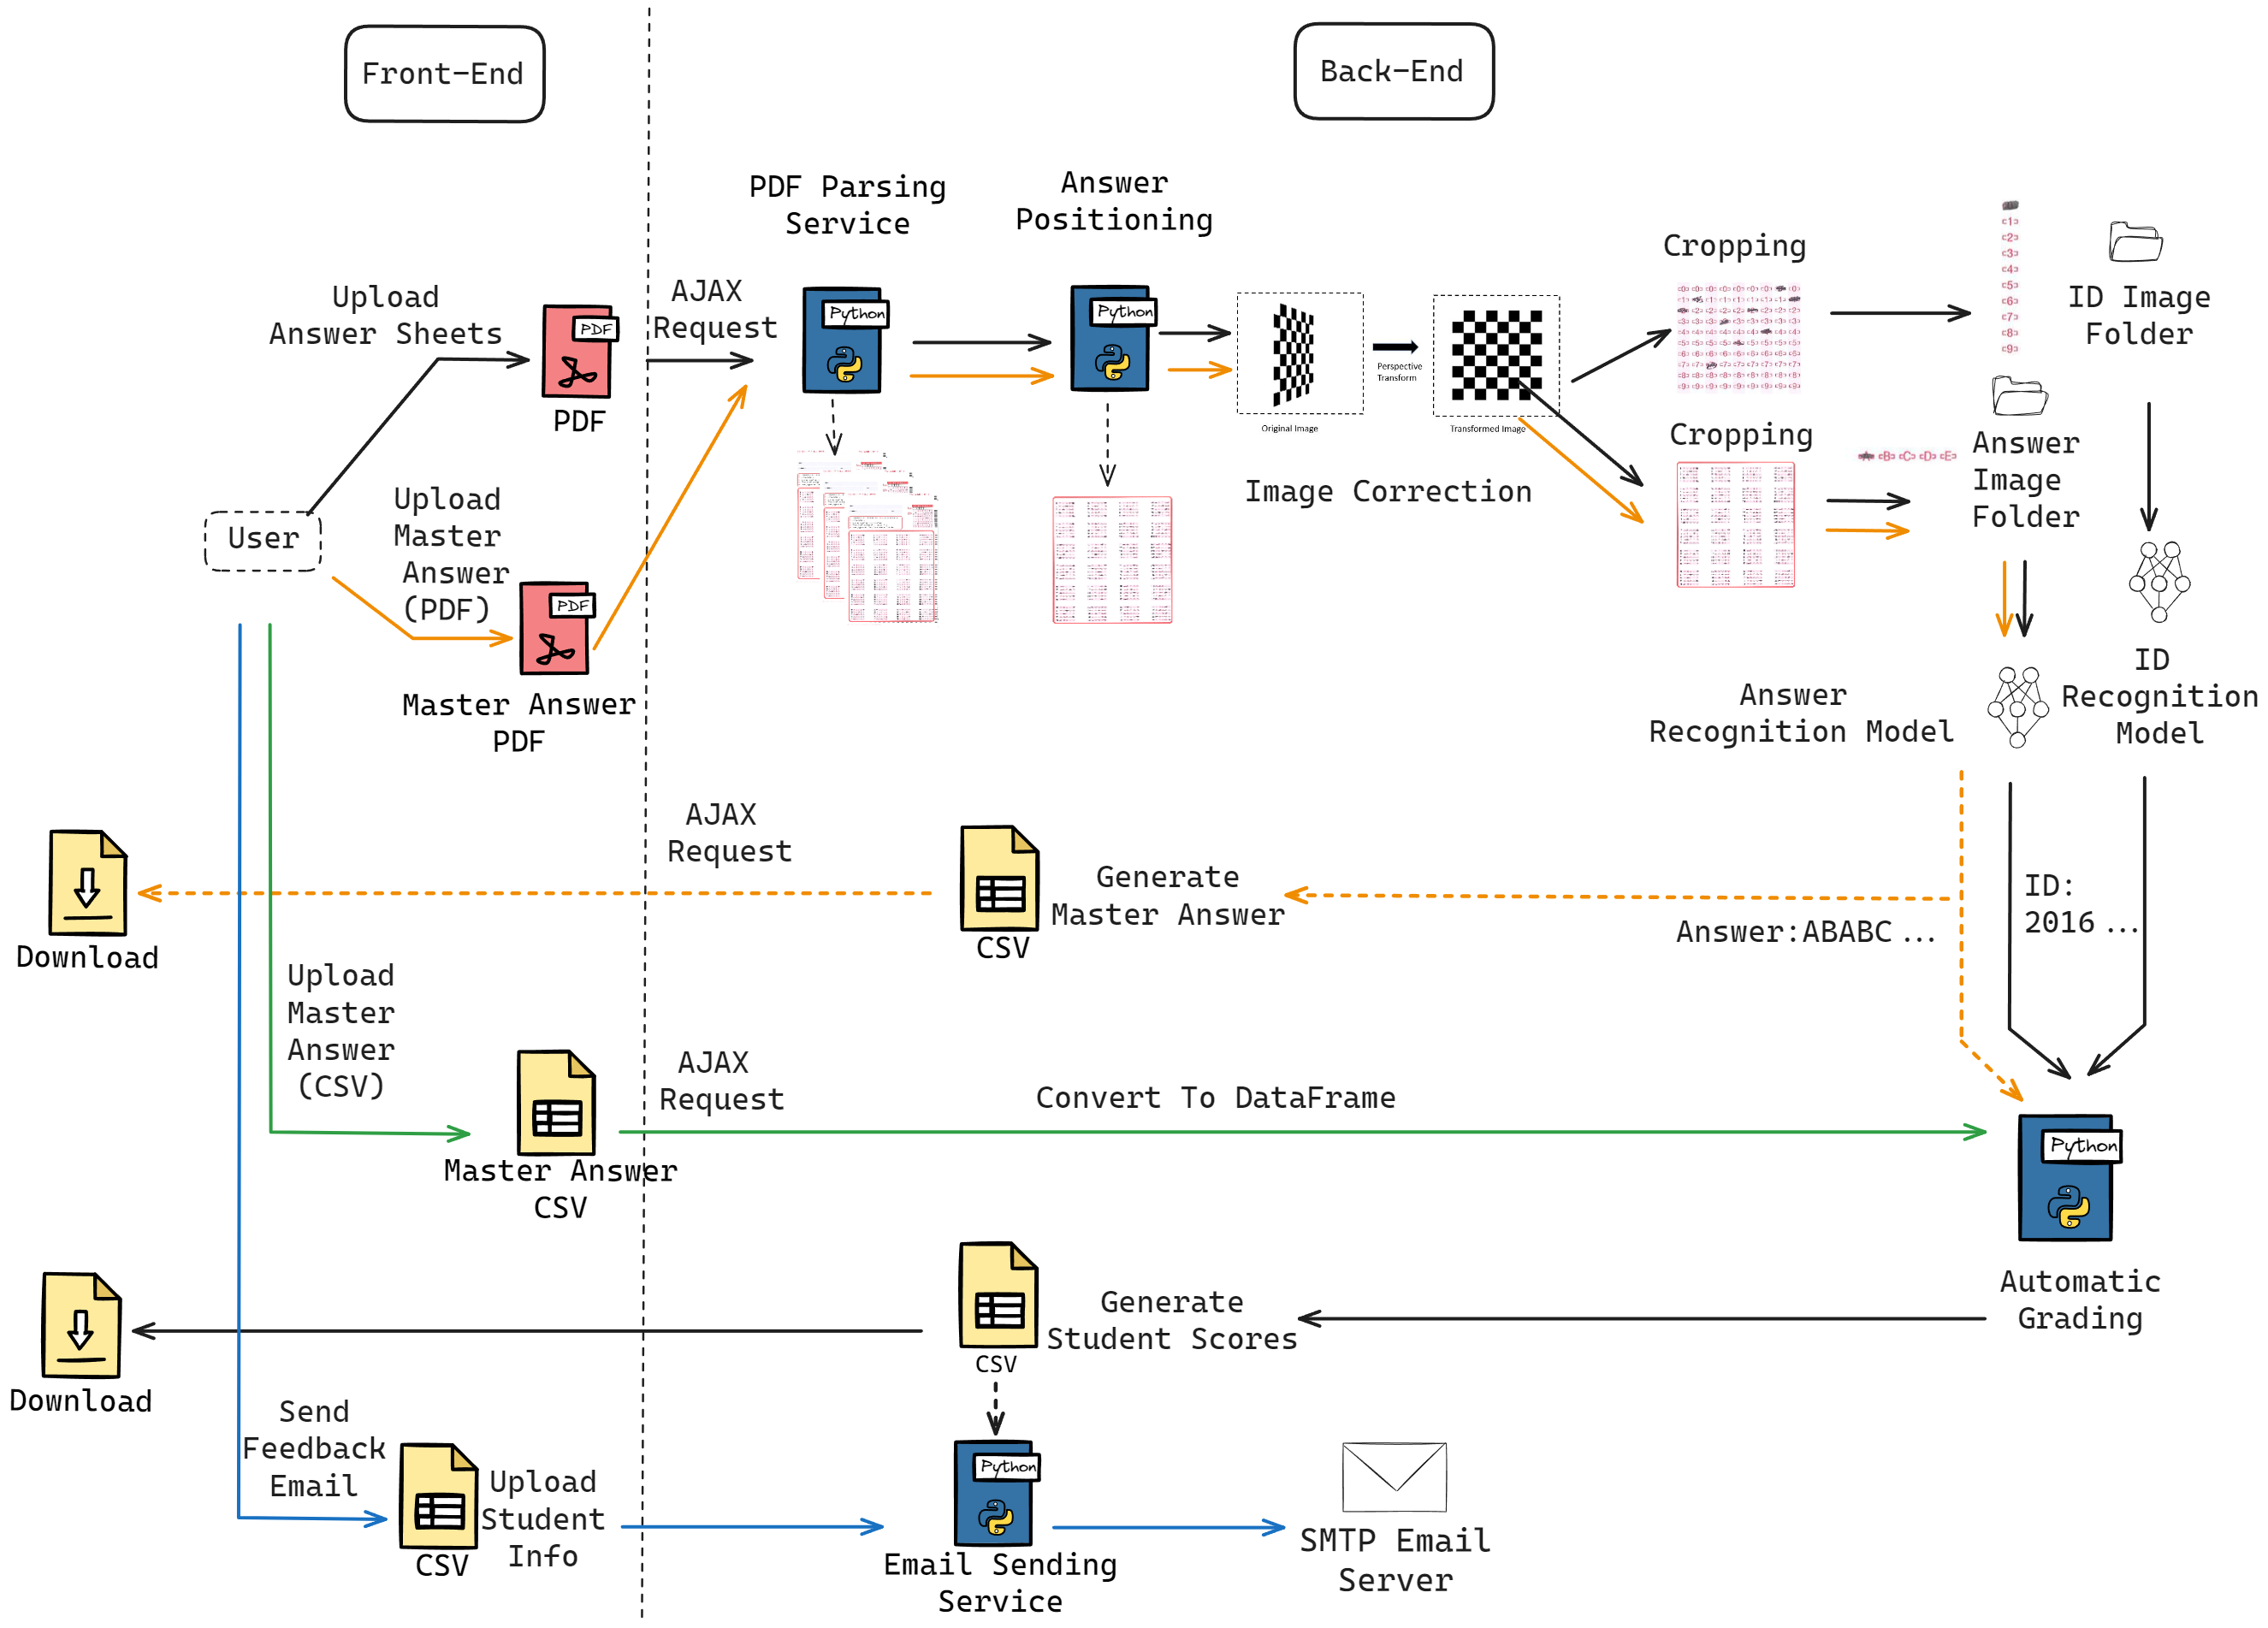
\includegraphics[width=0.8\textwidth]{Architecture.png}
    \caption{Overview of the system architecture.}
    \label{fig:architecture}
    \end{figure*}


    \subsection{Image Processing}
    The image processing part mainly involves four modules: PDF conversion,target area positioning, image correction \& enhancement and cropping.
    \begin{itemize}
        \item \textbf{PDF Parsing Service:} The uploaded PDF files are converted to images using the PyMuPDF library. The images are then passed to the image processing module.
        \item \textbf{Answer Positioning:} The images are cropped to extract the student ID and answers. The student ID is located in the upper right corner of the answer sheet, and the program needs to crop out the ID area based on anchor points. Answers are extracted by cropping the image based on the coordinates of the bounding rectangle.
        \item \textbf{Image Correction} The image containing the answer area will undergo a series of image processing functions, including perspective transformation, rotation correction, elimination of curve edges, and resizing, to ensure that the resolution and size of each image containing the answer area are exactly the same, and there are no deviations that affect subsequent cropping operations.
        \item \textbf{Cropping:} Use a cropping function and a loop to crop out answer for each question and the student ID for CNN model training and recognition. 
    \end{itemize}
    \subsection{Neural Network Model Design}
    As mentioned in Chapter 1.2, due to some previous related work in this field achieving good recognition results using neural network models with different architectures, this project will first conduct a pre-experimental process to find the most suitable model structure. These neural network models will all be trained with the same parameters, while ensuring that the number of convolutional layers is generally close. At the same time, the time required for each neural network to predict the images will also be taken into account, and finally, the best accuracy and running speed will be combined to select a suitable model. The neural network models tested in this project include:
    \begin{itemize}
        \item \textbf{Standard CNN:} A standard CNN model with 8 convolutional layers and pooling layers. This model will be used as a baseline for comparison with other models.
        \item \textbf{ShuffleNet:} A lightweight CNN model that uses group convolution and channel shuffling to reduce computational complexity. This model is designed for efficient operation in resource-constrained environments.
        \item \textbf{ResNet:} A deep CNN model with residual connections that allow for the training of very deep networks. This model is known for its high accuracy and performance on image recognition tasks.
        \item \textbf{VGG-16:} A deep CNN model with 16 layers that has been widely used for image recognition tasks. This model is known for its simplicity and effectiveness in feature extraction.
        \item \textbf{AlexNet:} A deep CNN model with 8 layers that was one of the first models to demonstrate the effectiveness of deep learning on image recognition tasks. This model is known for its simplicity and effectiveness in feature extraction.
    \end{itemize}
    The specific experimental details will be described in the next chapter. After selecting the appropriate model, a series of more detailed optimization schemes will be implemented, including increasing the number of layers of the neural network, optimizing hyperparameters, longer training time, using different schedulers, gradient descent, and other methods to improve the accuracy of the model.

    It should be noted that this project will use two different neural network models for answer recognition and student ID recognition, respectively. The model used for answer recognition supports 6 types of inputs, including 5 answer options and blank answers. The model used for student ID recognition supports 10 types of inputs, including 10 student ID number options. These models will be stored in the models.py file for comparison.
    \subsection{Model Training}
    The model training process will be divided into two parts: training the model for answer recognition and training the model for student ID recognition. The training process will be conducted on a dataset of labeled MCQ sheets. The dataset will contain over 1000 labeled MCQ answers for training and testing. The training process involve the following steps:
    \begin{itemize}
        \item \textbf{Dataset Creation:} The dataset will be preprocessed using the crop functions mentioned in previous chapters to extract the student ID and answers from the MCQ sheets. The data will be split into training and testing sets.
        \item \textbf{Model Training:} The models will be trained using the training set and tested using the testing set. The training process will involve feeding the input data into the model, calculating the loss, and updating the model parameters using backpropagation. All models will be trained using the same parameters, including the number of kernels, epochs, etc. Some pre-trained models are already built into the PyTorch library, including VGG and ResNet. During initial training, these pre trained models will be used and better results will be observed.
        \item \textbf{Model Evaluation:} The models will be evaluated based on their accuracy, precision, recall, and F1 score. The models will be compared based on their performance on the testing set. The model with the highest accuracy and F1 score will be selected as the final model.
        \item \textbf{Model Optimization:} The selected model will be further optimized using techniques such as hyperparameter adjustment, data augmentation, and transfer learning. The goal is to improve the model's performance and generalization ability.
    \end{itemize}
    \subsection{Website Architecture}
    The front-end of the website is designed to be user-friendly and intuitive, allowing users to easily upload answer sheets and standard answer templates, view and download results, and send feedback emails. The uploaded files (PDF and CSV) are sent to the server via AJAX. The server processes the uploaded files and returns the results to the user. The front-end design is based on HTML, CSS, and JavaScript, with the website built using Node.js. The front-end design includes the following components: 
        \subsubsection{Client-Side (Frontend)}
        This part of the system will be responsible for interacting with the users (students and instructors). 
        \begin{itemize}
            \item \textbf{Homepage:} The homepage allows users to upload answer sheets and standard answer templates in PDF/CSV format. The homepage also provides a preview of the uploaded files and allows users to delete or re-upload files if necessary. Users can click on the "Analyse" button to process the uploaded files, and once the analysis is complete, the results will be downloaded and also displayed on the analysis page.
            \item \textbf{Analysis Page:} The analysis page displays the results of the uploaded answer sheets, including the student's name, accuracy, student ID, and overall score. The page also displays the number of correct and incorrect answers, the score for each part of the test, and the rank of questions based on overall accuracy. The page also provides an option to download the results and send feedback emails to candidates, as well as student information configuration settings.
            \item \textbf{PDF Processing:} For answer sheet uploads, it stores the file and triggers the PDF parsing service. The PDFs are first converted to images and cropped to extract the student ID and answers. The cropped images are pre-processed to enhance the quality and remove noise. The images are deskewed and cropped to extract the student ID and answers.
            \item \textbf{Answer Recognition:} The pre-processed images are passed to a pre-trained model to extract the student ID and answers.
            \item \textbf{Scoring:} The extracted answers are compared with the master answer key to calculate the score.
            \item \textbf{Feedback:} Return a dataframe with student ID, mark, number of incorrect correct answers, and answers. The extracted IDs and answers are then written into a CSV file, student\_score.csv.The final output files can also be converted into text format and sent to the corresponding students using SMTP email server.
            \item \textbf{Infrastructure Workflow:} The server can be hosted on a cloud platform (AWS, Azure, etc.) and is managed using Docker containers. The server is deployed using a Flask application.
        \end{itemize}


        \subsubsection{Server-Side (Backend)}
        This part of the system will be responsible for processing the uploaded files, extracting student IDs and answers, comparing the answers with the standard answer key, and generating the results. The backend design includes the following components:
        \begin{itemize}
            \item \textbf{PDF Processing Service:} The PDF processing service converts the uploaded PDF files to images and passes them to the image cropping module. The service also stores the uploaded files and triggers the PDF parsing service.
            \item \textbf{Image Cropping:} The images are cropped to extract the student ID and answers. The images are first cropped into large answer area, followed by deskew and prospective transformation to obtain a fixed size raw image. Next, use a loop to cut all the question sheets in the answer area into one image and store them separately in a folder according to each page. The cropped images are pre-processed to enhance the quality and remove noise. 
            \item \textbf{Answer Recognition:} The pre-processed images are passed to a pre-trained model to extract the student ID and answers.
            \item \textbf{Scoring:} The extracted answers are compared with the master answer key to calculate the score.
            \item \textbf{Feedback:} Return a dataframe with student ID, mark, number of incorrect correct answers, and answers. The extracted IDs and answers are then written into a CSV file, student\_score.csv.The final output files are converted into text format and sent to the corresponding students using SMTP email server.
            \item \textbf{Infrastructure Workflow:} The server is hosted on a cloud platform (AWS, Azure, etc.) and is managed using Docker containers. The server is deployed using a Flask application.
        \end{itemize}

    \subsection{User Interface}
    As mentioned in the previous chapters, the user interface of the website mainly consists of a homepage and an analysis page. The interaction process required for such a program is relatively simple, generally only following the standard linear interaction process is required. I will refer to the UI design draft from the detailed proposal here, which differs from the final result in some aspects, especially in analyzing the page, but generally follows the same design language. The analysis page is invisible without any user action. Only when the website completes a user uploaded analysis will a "view results" button appear on the webpage, and clicking this button will redirect to the analysis results page. At this point, the user can directly rollback or reload to return to the homepage in order to start the next upload.
            
    \begin{figure*}
        \centering
        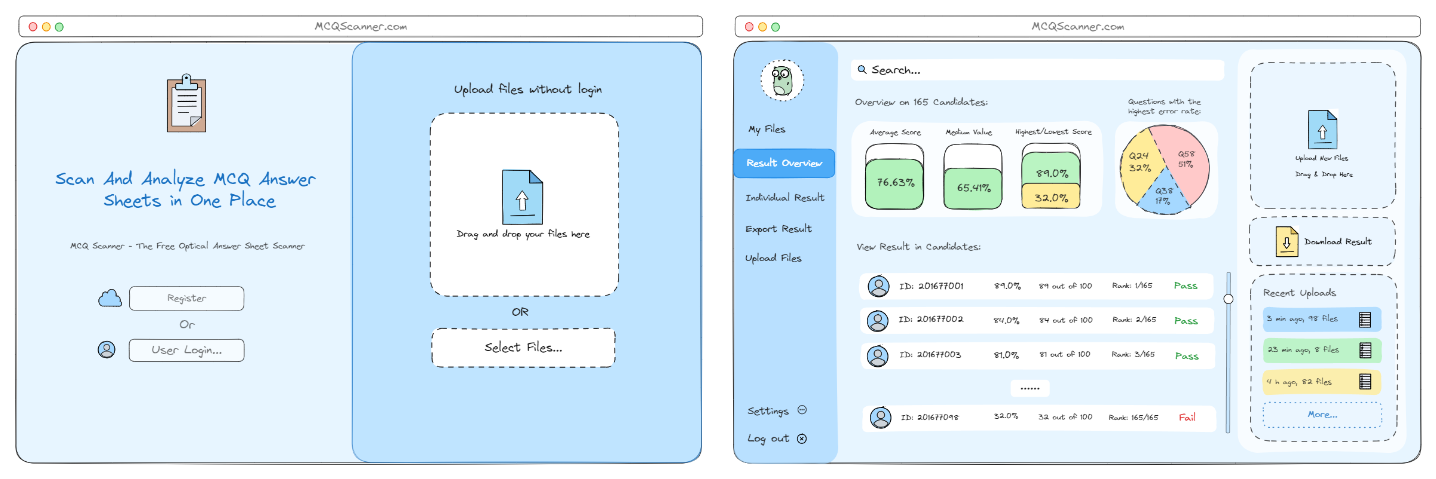
\includegraphics[width=0.9\textwidth]{UI_design.png}
        \caption{The user interface design of the website.}
        \label{fig:UI}
    \end{figure*}
    
    \subsection{Web Security}
    Implementing security measures is crucial for a website that processes exam answer sheets. Given the sensitive nature of the data (student IDs, exam answers, etc.), securing the application against various threats is essential: 
    \begin{itemize}
        \item \textbf{Data Encryption:} All data transmitted between the client and server should be encrypted using HTTPS. This will prevent eavesdropping. Obtain an SSL certificate from a trusted certificate authority (CA).
        \item \textbf{Input Validation:} Validate all user inputs to prevent SQL injection, cross-site scripting(XSS), and other common attacks.Implement a file size limit and use libraries that can inspect the file content.
        \item \textbf{Role-Based Access Control:} Implement Role-Based Access Control (RBAC) to ensure users only access data and features they are authorized for. Define roles such as "instructor" and "admin", and assign appropriate permissions.
        \item \textbf{Infrastructure Security:} Secure the server infrastructure by using firewalls, intrusion detection systems, and regular security audits. Use DDoS protection services like AWS Shield or Cloudflare to mitigate denial-of-service attacks.
        \item \textbf{API Key Management:} Secure API endpoints with API keys or tokens. Use OAuth for authentication and authorization. Limit the number of requests per API key to prevent abuse.
        \item \textbf{Regular Updates:} Keep all software and libraries up-to-date to patch security vulnerabilities. Regularly update the operating system, web server, and database server.
        \end{itemize}
        It should be noted that due to the Data and participant category restrictions of this project, the website is unable to provide the creation of usernames and login operations. \textbf{But all files are completed locally, and the server only retains the cropped images of individual questions and individual student numbers. These images will no longer contain personal information after being scrambled.} At the same time, the server will clear all caches after each processing is completed, ensuring that no personal data is stored on the remote server.
    \subsection{Data Structure}
    The data structure of this project is relatively simple, mainly including the following parts:
    \begin{itemize}
        \item \textbf{Image Data:} Image data is stored in three formats in the program. When converting PDF to image, \textbf{the converted image is stored in memory as a PIL image object. Subsequently, they are converted into numpy arrays for cropping and preprocessing operations. After cropping is completed, all images are stored in the cache folder in JPG format.} The purpose of this step is to reduce memory consumption. Due to the fact that each PDF file can easily generate thousands of cropped images, storing them in the cache area of the hard drive can save server memory and facilitate me to check the effectiveness of image cropping during the development process. Although this reduces the running speed of the software. When provided to the model for inference, they will be converted back into numpy arrays and removed from the cache
        \item \textbf{Model Data:} The model data includes the weights and biases of the neural network model. The model is trained using the image data and the labeled MCQ sheets. The model data is stored in a .pt file.
        \item \textbf{Answer Data:} After the answer and student ID recognition are completed, they will be stored in two forms. When the backend program uses the model to infer answers and student ID images separately, it will return a list containing only the inference results of the answers or student IDs. Subsequently, these two lists are passed into the result generation program. The result of the reasoning here will be processed in a series of ways, including calculating grades and accuracy, marking mistakes, and assigning weights. At the same time, each student's answer will also be assigned to their corresponding student ID. Finally, the program returns a pandas dataframe that contains all student and grade information. These information will be written as the result to the CSV file in the next function, and then passed to the front-end for users to download.
        \item \textbf{CSV Data:} The CSV data includes the student ID, mark, number of correct answers, and answers. The CSV data is generated by comparing the extracted answers with the master answer key.
        \item \textbf{Email Data:} The email data (CSV format) includes the student ID, real name and their email address. The email data is sent to the corresponding students using an SMTP email server.
    \end{itemize}
    \subsection{Error Handling}
    Error handling is crucial for building robust software. In this project, error handling will be implemented at various levels to ensure that the software can gracefully handle unexpected situations. The error handling mechanisms will include:
    \begin{itemize}
        \item \textbf{Input Validation:} The user might upload an incorrect file format or a corrupt file.The methods to solve this problem include restricting file formats, displaying a user friendly error message for incorrect formats, and limiting the maximum file size to prevent excessive large uploads.
        

\begin{lstlisting}[language=Python, caption=Input Validation Example]
    const allowedExtensions = ['pdf', 'csv'];
    const fileExtension = file.name.split('.').pop();
    if (!allowedExtensions.includes
    (fileExtension)) {
        alert('Only PDF and CSV files are allowed.');
        return false;
    }
    if (file.size > 100 * 1024 * 1024) { # 100 MB limit
        alert('File size exceeds the limit of 100 MB.');
        return false;
    }
    return true;
\end{lstlisting}


        \item \textbf{Exception Handling:} Use try-except blocks to catch exceptions and handle errors gracefully. Log the error messages to a log file for debugging purposes.
        \item \textbf{Error Messages:} Provide informative error messages to users when an error occurs. The error messages should be clear and concise, indicating what went wrong and how to fix it.
        \item \textbf{Error Logging:} Log all errors to a log file for debugging purposes. Include the timestamp, error message, and stack trace in the log file.
        

\begin{lstlisting}[language=Python, caption=Error Logging Example]
import logging

logging.basicConfig(filename='app.log', level=logging.ERROR)

try:
    # Code that might raise an exception
    pass
except Exception as e:
    logging.error(f"An error occurred: {e}")
\end{lstlisting}


        \item \textbf{Degradation:} Implement graceful degradation to ensure that the software can continue to function even if certain components fail. For example, if the image processing module fails, the software should still be able to process other components.
    \end{itemize}

    \subsection{Workflow \& Summary}
    \begin{itemize}
        \item \textbf{ Requirement analysis and planning:} Determine the goals and requirements of the project, including accuracy requirements for answer sheet identification, performance indicators, user interface design, etc. Develop a project plan to clarify the development timeline and resource requirements.
        \item \textbf{Data collection and preparation:} Collect a large amount of answer sheet image data, including positive and negative samples for model training and testing. Label the data to identify the correct answers and areas on the answer sheet.
        \item \textbf{Data preprocessing:} Preprocess image data, including image cropping, scaling, denoising, and other operations to facilitate subsequent processing and model training.
        \item \textbf{Feature extraction:} Extract features from the preprocessed image, which can include shape, contour, pixel distribution, etc. This project may also attempt to use deep learning methods for feature extraction.
        \item \textbf{Model selection and training:} Choose appropriate machine learning or deep learning models, such as convolutional neural networks (CNN). Train the model using training data and optimize model parameters to achieve accurate recognition of answer sheets.
        \item \textbf{Model evaluation and optimization:} Evaluate the model using test data to measure its performance and accuracy. If necessary, tune and improve the model.
        \item \textbf{Integrate into web pages:} Create a webpage front-end for users to upload question card images. The backend will receive images and call the trained model to identify the answer sheet. Display information such as recognition results and answer sheet scores. 
        \item \textbf{User interface design:} Design a user-friendly interface for users to upload question sheet images and view recognition results.
        \item \textbf{Testing and verification:} Conduct comprehensive testing of the entire system to ensure that it can function properly under different circumstances. Verify the accuracy and performance of the answer card recognition.
        \item \textbf{Deployment and Maintenance:} Deploy web pages to the server so that users can access them. Use continuous integration and continuous delivery (CI/CD) tools to automate the construction, testing, and deployment process. This helps to reduce human errors and improve deployment efficiency. Regularly maintain and update the system to ensure its continuous effectiveness. Configure HTTPS to provide secure data transmission.
        \item \textbf{Version control:} Use version control systems such as Git to track changes in project code. Host project code on online code hosting platforms (GitHub). Create branches to handle different functions and tasks for parallel development and tracking of the progress of each function, as well as regularly conduct code reviews to ensure code quality and consistency.
    \end{itemize} 

\section{Implementation}

    \subsection{Image Processing}
    Before starting this chapter, I would like to first state that the following content is the original contribution of the author unless otherwise stated or citing other work and literature.

    As mentioned in the previous chapters, the role of the image processing module is to process the PDF file input by the user in a series of ways, and finally output it as an image of a single question or student number option that can be recognized by the neural network model. The following image briefly illustrates how the answer is detected and cropped from the original image. The image processing module is implemented in the crop\_pdf\_input.py file. The file includes the following modules:
        \subsubsection{PDF Conversion}
        The operation of converting PDF into an image and scaling it is mainly achieved by the following two functions:
        \begin{itemize}
            \item \textbf{convert\_pdf\_to\_images():} The purpose of this function is to convert each page in the PDF file into an image. This function uses the PyMuPDF library to convert the PDF file into an PIL(Python Imaging Library) image object.
            \begin{figure}[ht]
                \centering
                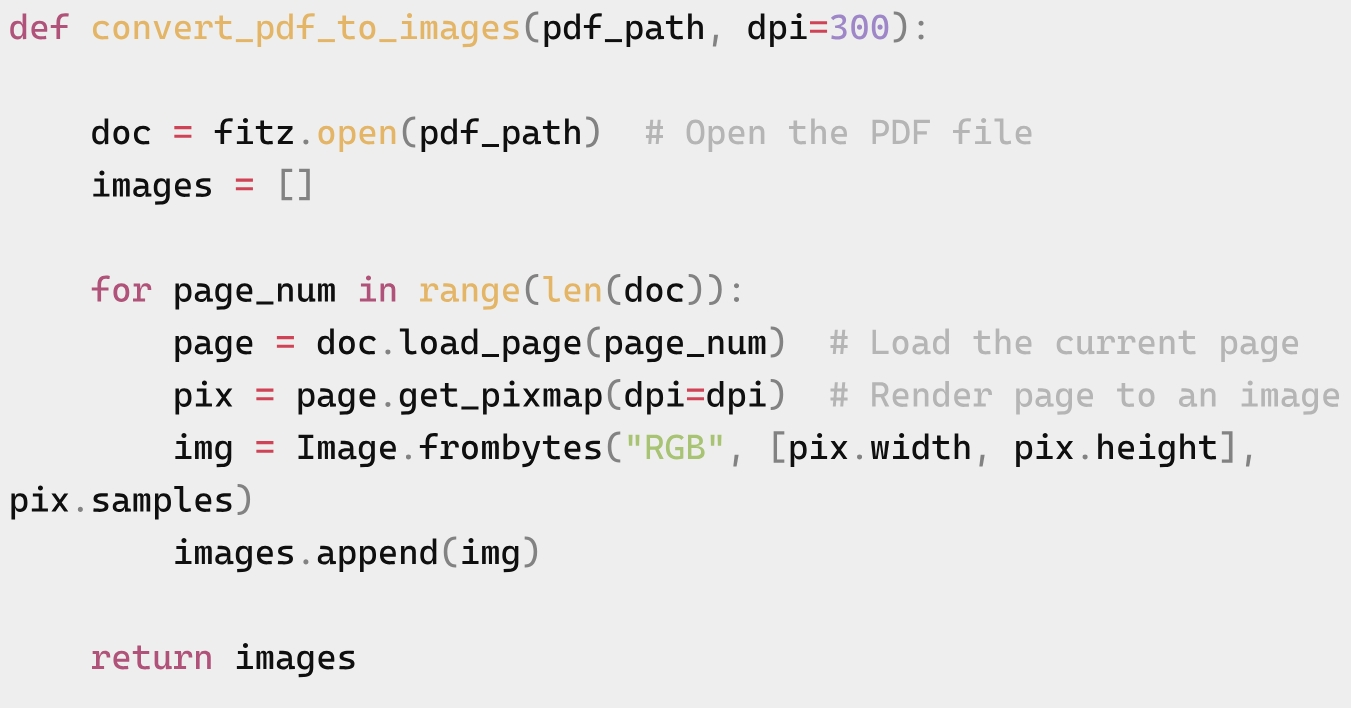
\includegraphics[width=0.48\textwidth]{code1.png}
                \caption{PDF conversion}
                \label{fig:example}
            \end{figure}
            \item \textbf{scale\_image:} The purpose of this function is to scale the PIL image proportionally and then convert it to an OpenCV format image, and also scales the image to a fixed size. The function takes the image object and the target size as input and returns the scaled image. After testing, a scaling ratio of 40\% is more appropriate. This makes the space occupied by the image relatively small and does not lose important information.
        \end{itemize}
        \subsubsection{Answer Positioning}
        How to locate the answer has always been a tricky issue in the early stages of this project. The key to this operation is not to rely on the black positioning square on the right side of the answer sheet to find the answer. In the initial plan, I attempted to train an additional neural network model to detect small square regions composed of five questions on the answer sheet. There are a total of 24 such areas on the test paper. The following image shows the images of these regions that I detected using a neural network during my first attempt. This convolutional neural network consists of three convolutional layers and three pooling layers, using object detection mode.

        \begin{figure}[ht]
            \centering
            \includegraphics[width=0.15\textwidth]{ans_detect.png}
            \caption{Early stage answer detection demo}
            \label{fig:ans_detect}
        \end{figure}

        In fact, this approach has many drawbacks. Firstly, using neural networks to detect answer regions can significantly reduce computational speed. Secondly, the size of the answer regions detected by the neural network is not consistent. It will be very complex in subsequent processing. Therefore, the plan was quickly abandoned after simple testing. The current plan is to use plain OpenCV functions to detect the answer area. 

        After comparing similar projects and communicating with team members, \textbf{I ultimately decided to cut out the entire answer area by detecting the shape of the rectangle.} We noticed that there is a prominent red rectangle around the answers on the answer sheet, and this rectangle shape is the largest on the entire answer sheet. This gives us the opportunity to use the shape detection feature of OpenCV.

        \begin{figure}[ht]
            \centering
            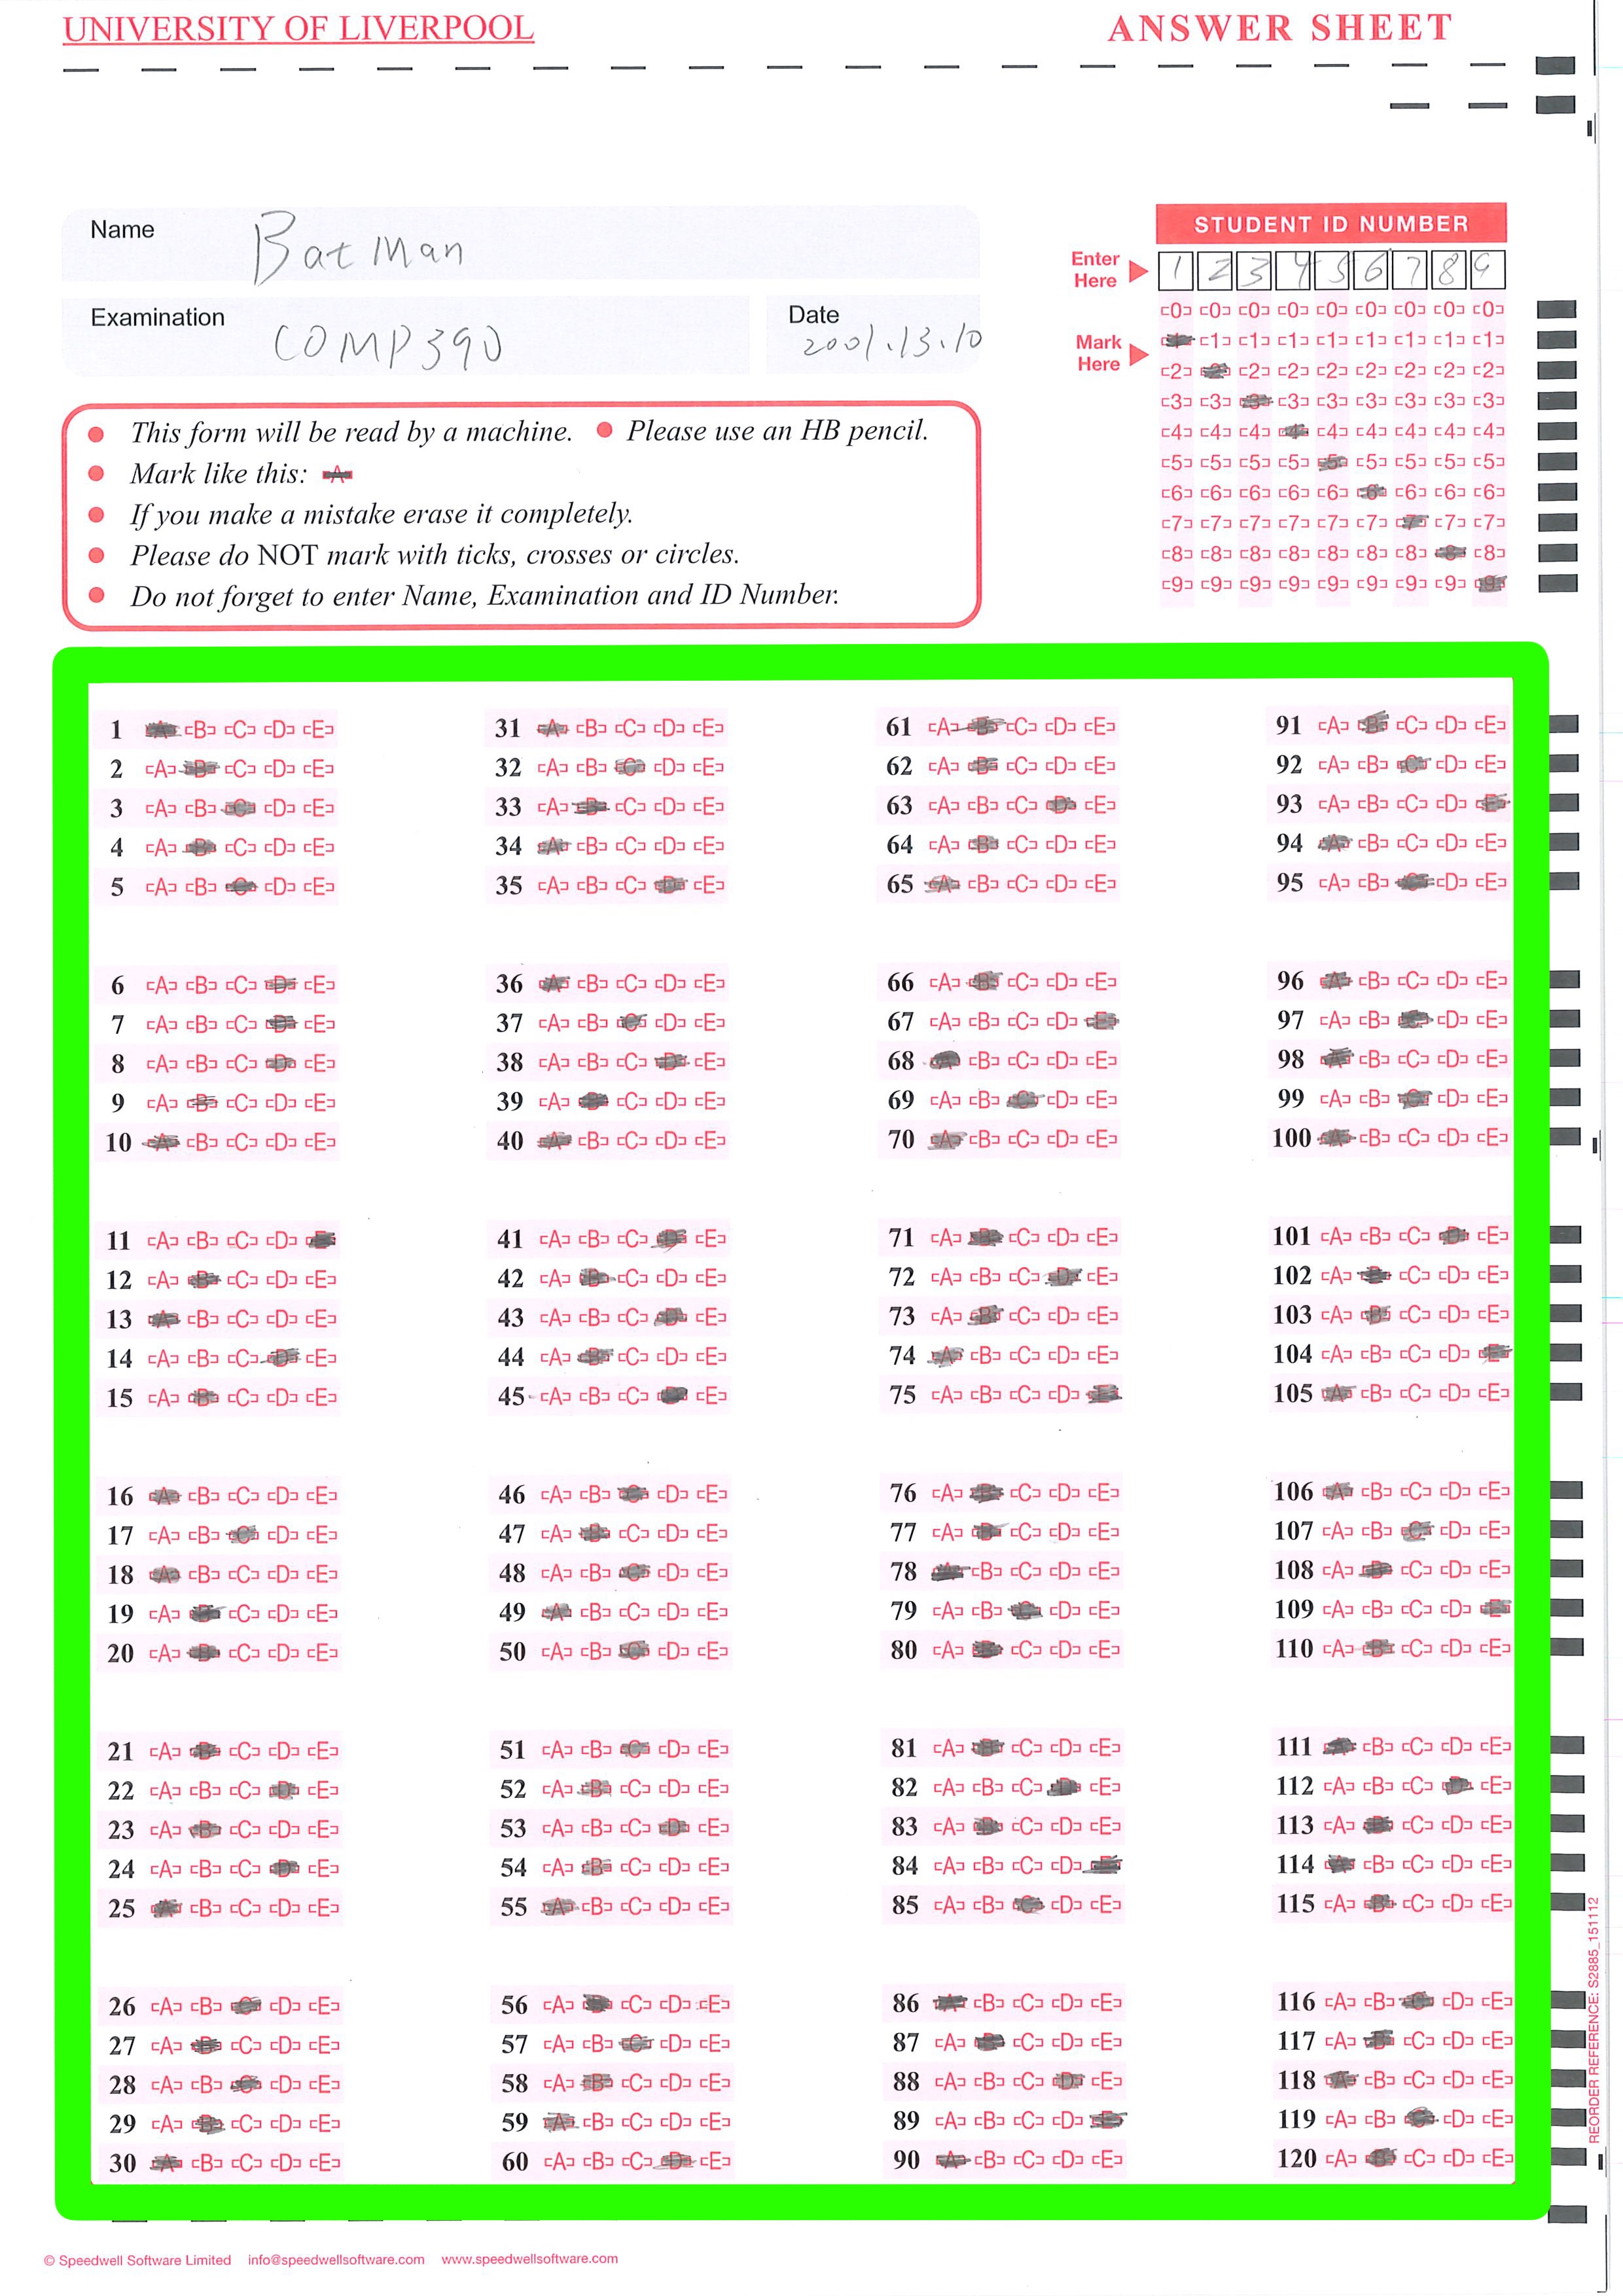
\includegraphics[width=0.15\textwidth]{countours.jpg}
            \caption{Answer area countour detection}
            \label{fig:countours}
        \end{figure}

        Firstly, we convert the image from the PDF processing function into a grayscale image, add Gaussian blur to it, and then use a Canny() edge detector to extract edges. Meanwhile, use the edge\_detect() function to perform edge detection on the image and then search for external contours. The function uses the cv2.findContours() function to find the contours of the image. The function then sorts the contours by area and selects the largest contour as the answer area, and returns the coordinates of the bounding rectangle of the answer area. Figure \ref{fig:countours} shows the contour detection process.

        
        \subsubsection{Image Rectification}
        Due to the tendency of the test paper to have some offset when scanning as a PDF file, such as slight rotation, upside down placement, etc., it is necessary to perform image correction on the cropped area and scale each image to a fixed resolution for subsequent cropping of individual answers. Image correction mainly consists of three parts: rotation correction, perspective transformation, and flipping correction. These operations are performed by the crop() function and the deskew() function.

        The crop() function uses the previous edge detection function to find the maximum external contour of the image, calculate its minimum bounding rectangle, and then crop out the answer area and ID area based on the rectangle. The deskew() function calculates the tilt angle of the image and rotates it for correction, then crops out the answer area and ID area.

        The deskew() function first performs a perspective transformation on the image. It projects a specified plane through a projection matrix, thereby eliminating image distortion caused by perspective.This feature is implemented using the cv2.warpPerspective() function.

        \begin{figure}[ht]
            \centering
            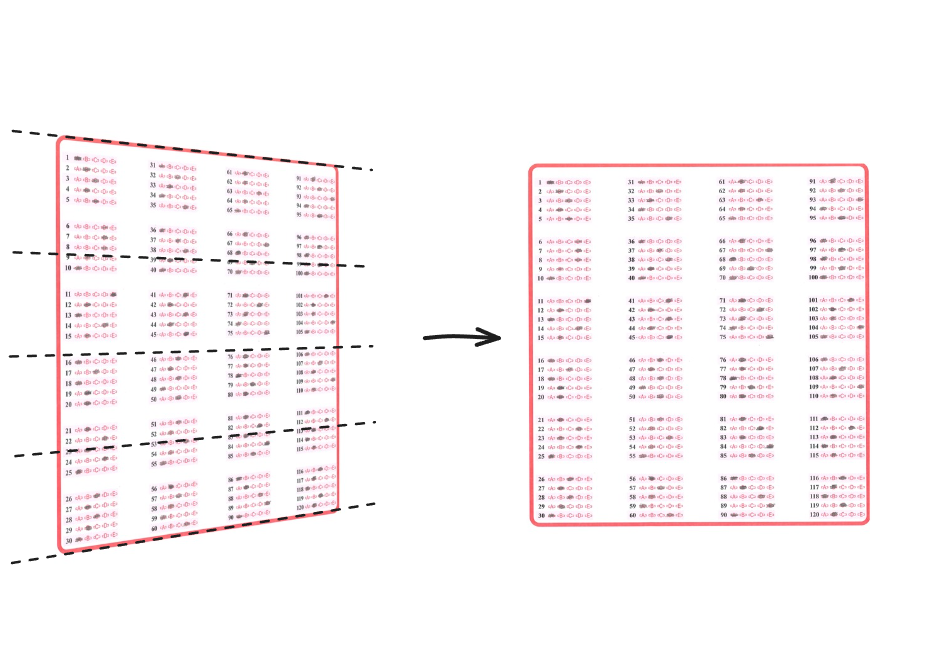
\includegraphics[width=0.4\textwidth]{perspective_transform.png}
            \caption{Perspective transformation}
            \label{fig:perspective_transform}
        \end{figure}

        When the scanned PDF file has a slight tilt (such as 5°-20°), the deskew() function can also effectively rotate the image to the correct position using the following steps:
        \begin{itemize}
            \item \textbf{Find contours:} 
            
            Firstly, the function calls find\_contours(image) to find the external contours in the image. The find\_contours function uses Canny edge detection to find edges.

            \item \textbf{Calculate the Minimum Bounding Rectangle:}
            
            Then the function finds the maximum contour $c$ (using cv2. contourArea to determine the contour area). The function cv2. minAreaRect(c) is used to calculate the minimum bounding rectangle $rect$ of the contour and obtain the rotation angle angle. The width and height of the rectangle also provide information to help determine how to rotate the image.

            \item \textbf{Angle Correction:} 
            
            If the width of the rectangle is greater than the height $(rect [1] [0]>rect [1] [1])$, it indicates that the rectangle is horizontal, and the angle needs to be adjusted to 90+angle. This angle represents the rotation angle of the image relative to the horizontal direction.

            \item \textbf{Rotation:}
            
            Generate a two-dimensional rotation matrix $M$ using the cv2.getRotationMatrix2D function. Center represents the rotation center point, angle is the rotation angle, and $1.0$ is the scaling ratio. Use the cv2. warpAffine function to apply the rotation matrix $M$ and rotate the image to the corrected angle.

            \item \textbf{Cropping:}
            
            Finally, the function calls crop (rotated, contours, h, w) to crop the image. The crop function crops out the main parts of the image and the ID region based on the minimum bounding rectangle.

        \begin{figure}[ht]
            \centering
            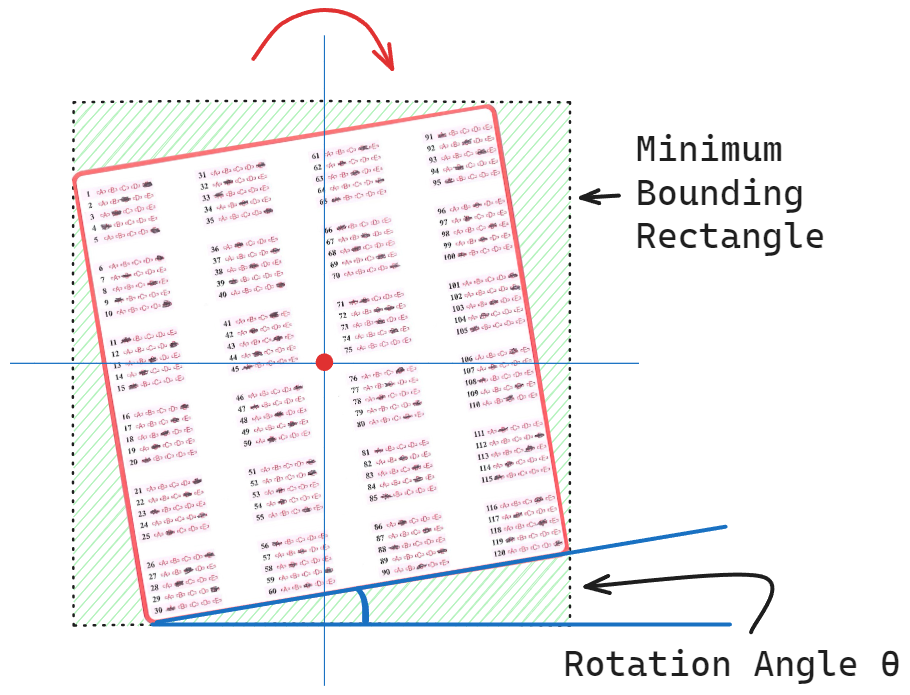
\includegraphics[width=0.4\textwidth]{deskew.png}
            \caption{A demosntration of deskew function}
            \label{fig:deskew}
        \end{figure}
        \end{itemize}
        When the tilt of the PDF image is greater than 90°, it means it has been placed upside down. At this point, we need to use another rotation method to rotate the image back to the correct angle. This feature is implemented in the crop() function. Due to the fact that the rectangular area containing the answer is different from the top distance y1 and the bottom distance y2 of the paper. The crop function compares these two distances before cropping, and if y1 is greater than y2, it indicates the answer sheet is placed correctly. Otherwise, the image is upside down. At this point, it will rotate the image 180° and compare these two distances again. If there is still an error, it will throw an exception.

        \begin{figure}
            \centering
            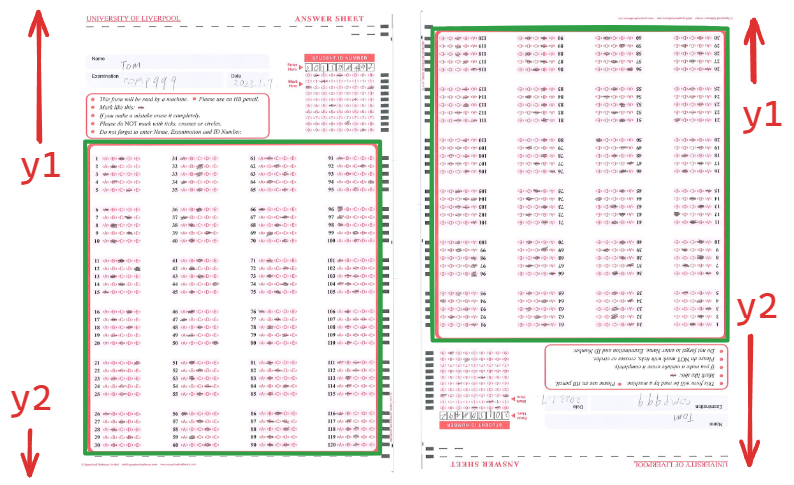
\includegraphics[width=0.4\textwidth]{ans_flip.png}
            \caption{Flipping correction}
            \label{fig:ans_flip}
        \end{figure}

        \subsubsection{Locate and crop the ID area}
        The answer area can be easily cropped using contour matching, but the area where the student ID is located does not have a clear rectangular contour. Therefore, anchor points were used to determine its position when cropping the ID region. Since the rectangular coordinates of the previously cropped answer are always fixed, we use the vertex $X$ in the upper right corner of this answer region as the anchor to determine the position of the ID region.


        \begin{figure}[ht]
            \centering
            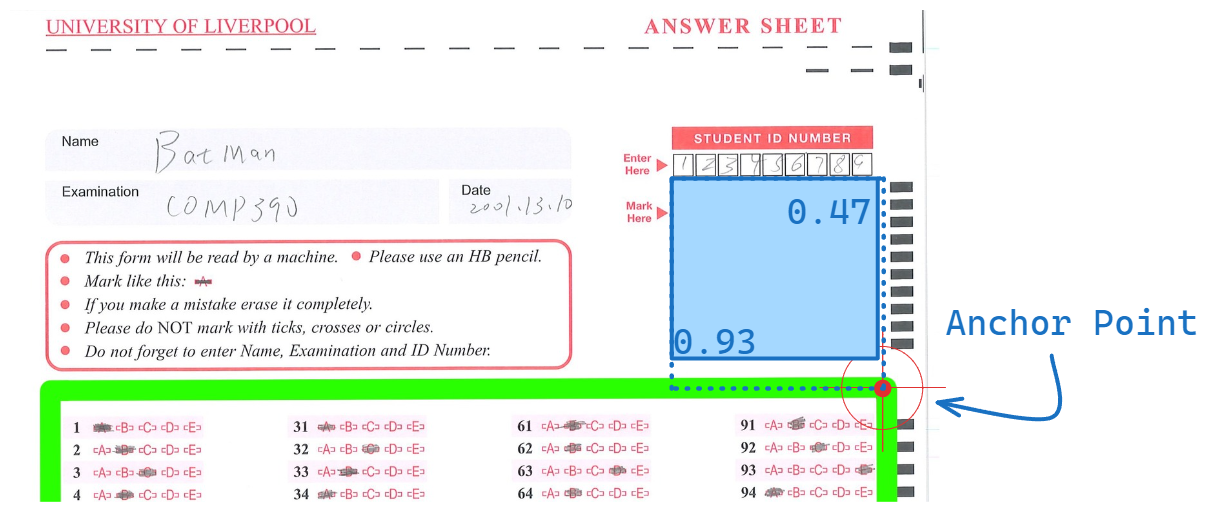
\includegraphics[width=0.4\textwidth]{locate_id.png}
            \caption{Locating the ID area with anchor points}
            \label{fig:locate_id}
        \end{figure}


        \subsubsection{Cropping Answers}
        After determining the area where the answer is located, the crop\_box() function and crop\_loop() function will crop out the answer for each question. Among them, crop\_box() crops a rectangular region in a given image, while crop\_loop() crops the ID region into a separate ID image through a nested loop. There is also a get\_num\_questions() function in this module, which is used to read the total number of questions in the CSV file uploaded by the user. The default is 120 (which is the maximum value of the test question). If it is less than this value, crop loop will be cropped according to the actual number of questions set by the user.
        
        \begin{figure}[ht]
            \centering
            
\includegraphics[width=0.2\textwidth]{ans.jpg}
            \caption{An example of a cropped answer}
            \label{fig:ans_example}
        \end{figure}
    
        At this point, all answers and student IDs have been cropped. In the main function, they will be stored in the corresponding student ID folder and answer folder, with the name of each folder is one-to-one, ensuring that the student ID matches its corresponding answer. \textbf{Full code for the image processing module can be found in the crop\_pdf\_input.py file in the appendix.}


    \subsection{Dataset}
    The main identification object of this project is the standard answer sheet of the University of Liverpool. However I did not use any datasets or APIs from public or non-public sources. This will be explained in the \textbf{Ethical Considerations} Section. During the training and testing stages, I use scanned copies of answer sheets made by myself and the team members as the dataset. Random answers were filled on blank answer sheet templates provided by the supervisor at the beginning of the project, along with random names and fake student ID numbers to simulate the real situation. In the image recognition algorithm section, the software needs to recognize the student's ID. Although fake data is used during training, this part of the content will also be deleted immediately after the results are generated to ensure the confidentiality of personal information.

    \textbf{In order to achieve higher accuracy in the model, the capacity of the dataset is an important consideration.} The dataset used in this project is a collection of labeled MCQ sheets. As mentioned in the previous chapter 2.2, the model requires a training set of more than 1,000 data and a test set of more than 100 data. The capacity of the data set we produced at the beginning of the project could not meet this requirement. After discussing with the team members, we decided to use the copied blank answer sheets to create a new data set. It should be noted that these data sets are filled in by group members on blank answer sheets and do not contain any personal information.
    
    \begin{figure}[ht]
        \centering
        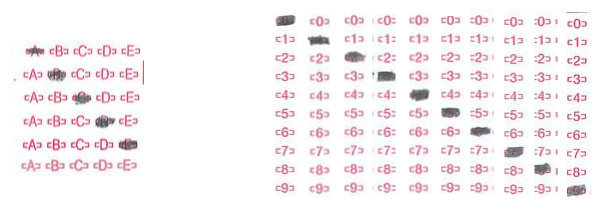
\includegraphics[width=0.3\textwidth]{dataset.png}
        \caption{An example of the dataset}
        \label{fig:dataset}
    \end{figure}

        \subsubsection{Answer Dataset}
        The training set of this data set comes from 60 answer sheets, and each 10 answer sheets fill in the same options, including a total of 6 categories, namely "A" "B" "C" "D" "E" "X" (X represents not filled in). Each answer sheet has 120 questions, which means 1200 data for each category.In addition to this, we also made a test set with 240 data for each category, which makes the ratio of test set to training set 1:5.

        To load the dataset, we use ImageFolder in PyTorch to load the dataset in DataLoader:

        \begin{figure}[ht]
            \centering
            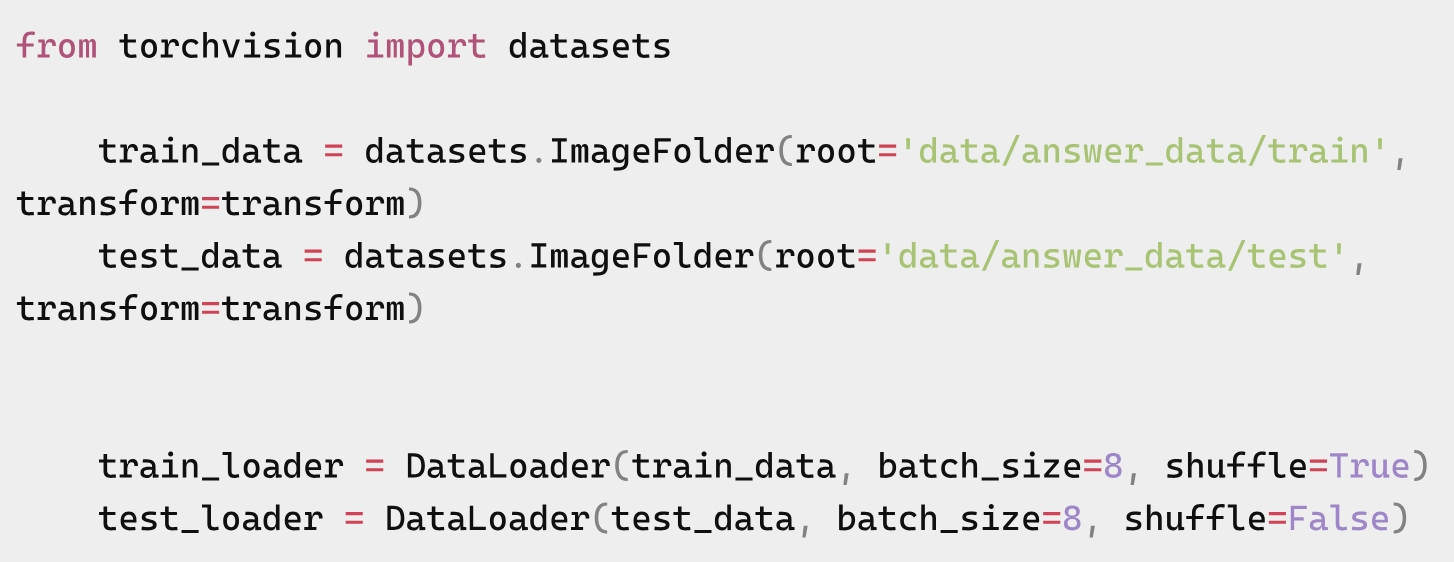
\includegraphics[width=0.48\textwidth]{dataloader.png}
            \caption{Loading the dataset in PyTorch}
            \label{fig:data}
        \end{figure}

        \subsubsection{Student ID Dataset}
        The student ID data set contains 10 categories, including "0", "1", "2", "3", "4", "5", "6", "7", "8", and "9". The data set is stored in the data folder in the project directory. The data set is also loaded using the ImageFolder class in PyTorch and passed to the DataLoader for training and testing.


    \subsection{Model selection}
    There are many factors to consider in finding a suitable model structure for this project. It involves the model's classification performance (that is, the highest accuracy that can be achieved), fitting speed, training speed, etc. Due to limitations of computing resources, we cannot support too long training duration and too slow fitting speed. In order to select the most suitable model for this project, \textbf{we will evaluate the following models: AlexNet, CNN, Wide ResNet, VGG-16 and ShuffleNet.}

        \subsubsection{Experiment Plan}
        In order to better evaluate the advantages and disadvantages of these model architectures, an experiment needs to be designed to evaluate the classification performance of AlexNet, CNN, Wide ResNet, ShuffleNet and VGG-16 on the answer data set. This experiment records the performance testing of different model architectures in the early stages of the project, so the model structure used is quite different from the final optimized model. To ensure that the variables are as consistent as possible, the model will use the same hyperparameters for training, such as learning rate, epochs, batch size, etc.

        \begin{itemize}
            \item \textbf{1. Data Preparation:} Load the answer data set and student ID data set using the ImageFolder class in PyTorch. Split the data set into training and testing sets.
            
            \item \textbf{2. Model implementation:} In order to ensure that the project can quickly test the model and the model can complete training in fewer epochs, the pre-trained model in torchvision.models is used here, and the last layer is modified to adapt to the six categories (ABCDEX).
            
        \begin{figure}[ht]
            \centering
            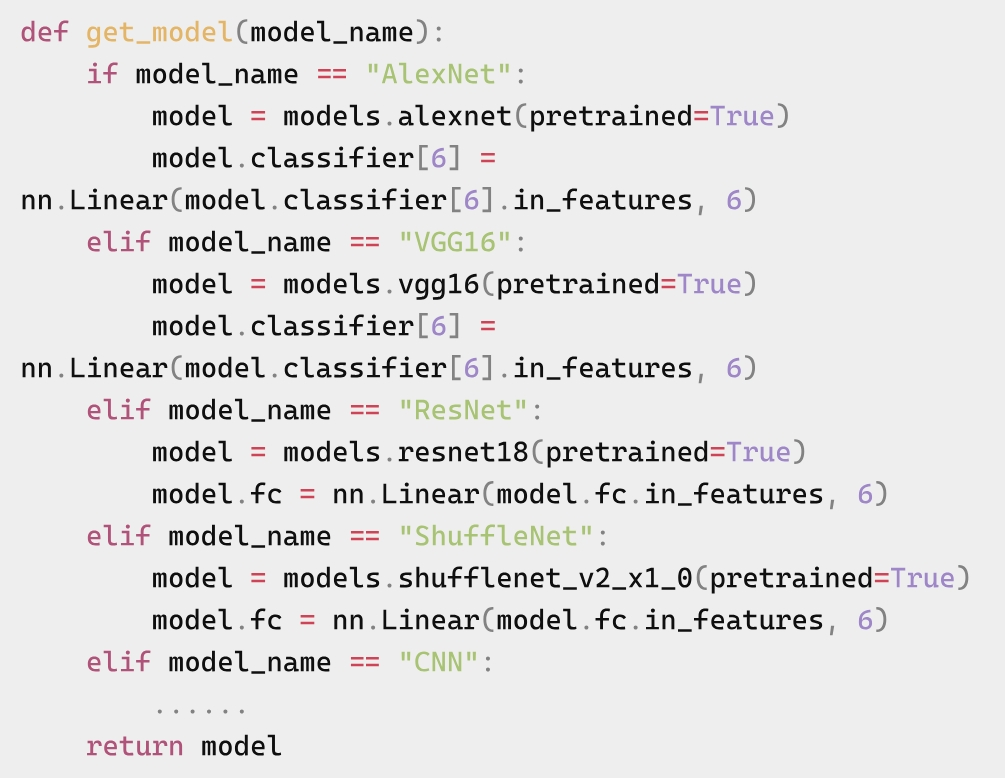
\includegraphics[width=0.48\textwidth]{model_select.png}
            \caption{Implementation of models}
            \label{fig:model_select}
        \end{figure}

            \item \textbf{3. Experimental setup:} Divide the data set into training set, validation set and test set. For each model, the training set is used for training, the validation set is used to tune hyperparameters, and the test set is used for final performance evaluation.

            Set appropriate hyperparameters such as learning rate, batch size, etc. Cross-validation can be used to evaluate performance more robustly. Train the model using the training set with same hyperparameters and clculate the accuracy, precision, recall, and F1 score of the model. 

        \begin{figure}[ht]
            \centering
            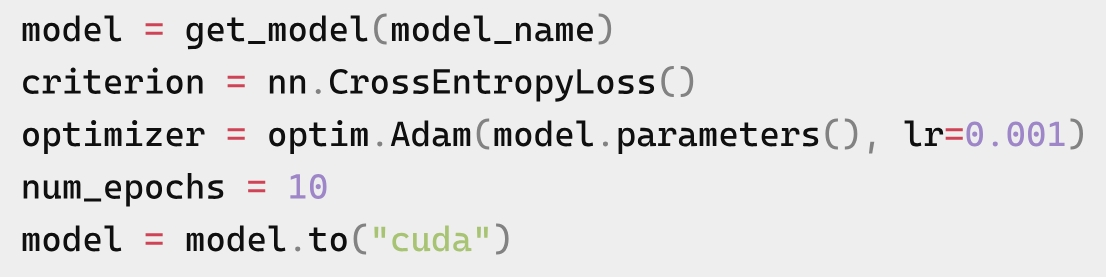
\includegraphics[width=0.48\textwidth]{hyperparameter1.png}
            \caption{Hyperparameter setting}
            \label{fig:hyperparameter1}
        \end{figure}

        \end{itemize}
        \subsubsection{Result}
        The results of the experiment are shown in the following table. The table shows the accuracy, precision, recall, and F1 score of each model on the answer data set. In this experiment, considering factors such as training time and accuracy, it can be seen from the chart that Wide ResNet performs the best. \textbf{Therefore, this project chooses to use Wide ResNet for subsequent improvements to improve performance.} At the same time, it can also be seen that the performance of the CNN model on this dataset is relatively stable, so this model will be used to test other modules added in the future.

        \begin{table}[h]
            \begin{tabular}{|l|l|l|l|l|l|}
            \hline
                     & Loss & Acc & Precision & Recall & F1  \\ \hline
            ShuffleNet    & 0.20  & 0.95 & 0.95 & 0.96 & 0.95         \\ \hline
            AlexNet     & 0.04 & 0.98 &  0.98 &  0.98 &  0.98      \\ \hline
            VGG-16 & 0.07  & 0.98 & 0.98 & 0.98 &  0.98      \\ \hline
            ResNet    & 0.02  & 0.99 & 0.98 & 0.99  & 0.98         \\ \hline
            CNN      & 0.06   & 0.99  & 0.98  & 0.99  & 0.98        \\ \hline
            \end{tabular}
            \caption{Basic Features}
            \label{tab:basic}
        \end{table}

        \begin{figure}[ht]
            \centering
            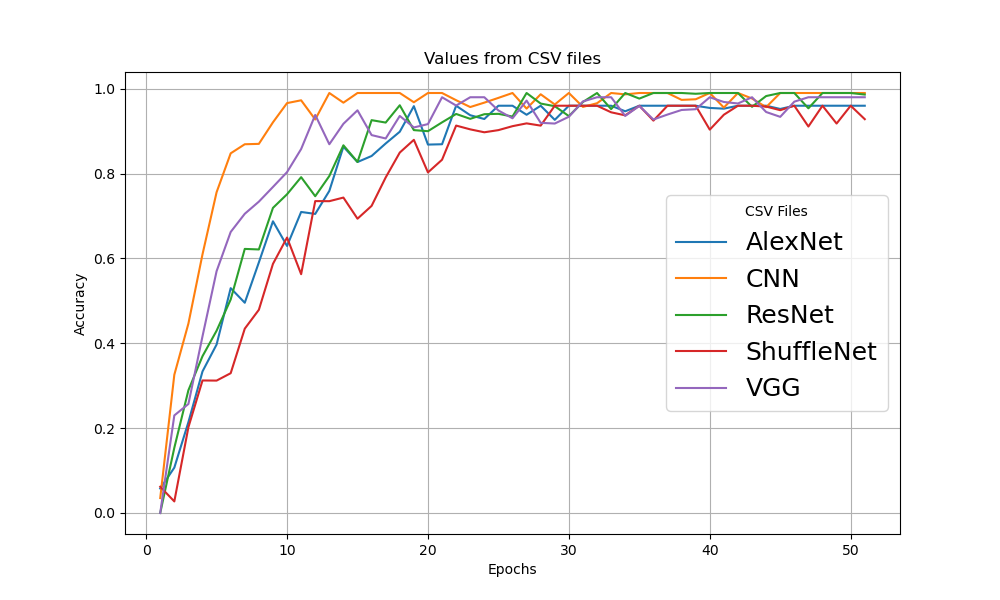
\includegraphics[width=0.48\textwidth]{fitting_curve.png}
            \caption{The fitting curve of different models}
            \label{fig:fitting_curve}
        \end{figure}


    \subsection{Model Implementation}
    In the previous chapter, Wide ResNet achieved good test results. It's an improvement of ResNet where the main difference between lies in the design of width and depth. 

    ResNet (Residual Network) was proposed by Kaiming He et al.\cite{resnet}, a researcher at Microsoft Research, in 2015. The core idea of ResNet is to introduce the concept of residual blocks or residual learning. In traditional neural networks, feature extraction is achieved by stacking multiple layers, but as the number of layers increases, problems such as vanishing and exploding gradients arise, making training difficult. Residual learning introduces shortcut connections in the network, making it easier for the network to learn residuals (residual information), thereby deepening the depth of the network\cite{wightman2021resnet}.

    Wide ResNet is an improvement and extension of ResNet, introducing the concept of "width" to increase the model width of the network and enhance learning ability\cite{zagoruyko2017wide}. The proposal of Wide ResNet mainly solves the balance problem between depth and width in ResNet, improving network performance by increasing the number of channels (width).

    The basic residual block structure of Wide ResNet is shown in figure \ref{fig:common_res_block}. This structure is based on the pre-trained model from the previous chapter. In the following sections, we will introduce the improved model structure for identifying answers.

        \begin{figure}[ht]
            \centering
            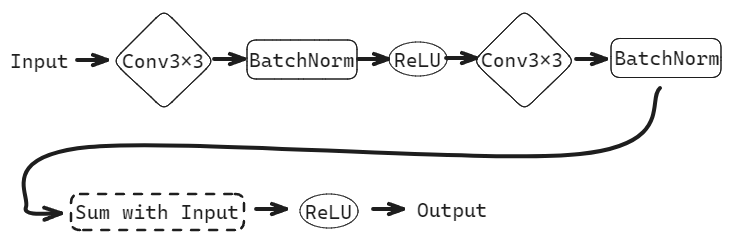
\includegraphics[width=0.48\textwidth]{common_res_block.png}
            \caption{Basic residual block structure}
            \label{fig:common_res_block}
        \end{figure}
    

    \subsubsection{Model Structure}
    The final model architecture used in this project is based on Wide-ResNet18. The architecture consists of two main components: `WideBasicBlock` and `WideResNet`. The `WideBasicBlock` is the basic building block of the model, and the `WideResNet` is the main model architecture that consists of multiple `WideBasicBlock` layers. The model is implemented using PyTorch and is stored in the models.py file. The model architecture is shown in figure \ref{fig:nn}.


        \begin{figure}[ht]
            \centering
            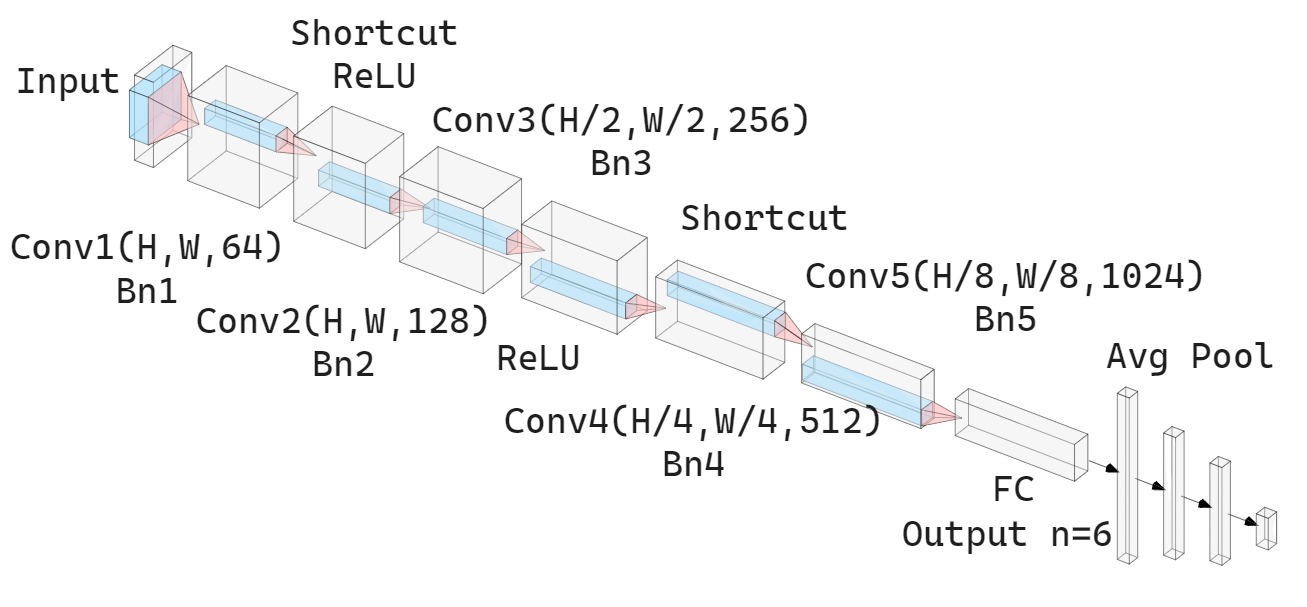
\includegraphics[width=0.48\textwidth]{nn.png}
            \caption{Architecture of the model used in this project}
            \label{fig:nn}
        \end{figure}
    \subsubsection{WideBasicBlock:} 
    
    The `WideBasicBlock` is the basic building block of the model. It consists of two convolutional layers with batch normalization and ReLU activation functions. The block also includes a residual connection that adds the input to the output of the second convolutional layer. The block is implemented as a class in PyTorch and is used to build the `WideResNet` model.
    \begin{figure}[ht]
        \centering
        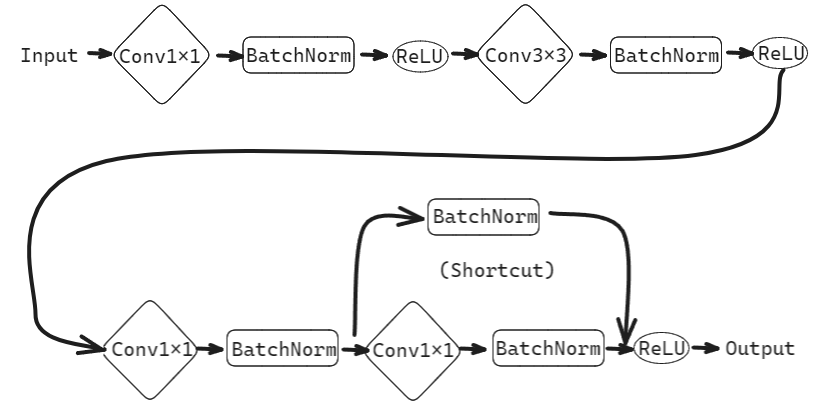
\includegraphics[width=0.48\textwidth]{custom_res_block.png}
        \caption{The improved structure of the residual block in the model.}
        \label{fig:custom_res_block}
    \end{figure}
    The `stride` parameter controls the down-sampling in the convolutional layers. The block also has a shortcut connection, which is used to match the dimensions of the input and output if there is a change in spatial resolution (stride != 1) or the number of channels (in\_channels != out\_channels * width). The `forward` method defines the forward pass of the block, incorporating residual connections.

    The structure of the residual block in the model is shown in figure \ref{fig:custom_res_block}.

    The forward propagation process of the basic residual block is as follows:
    \begin{enumerate}
        \item The input is convolved using Conv1x1.
        \item Batch normalization is performed through BatchNorm.
        \item Activate through ReLU.
        \item Perform 3x3 convolution through Conv3x3.
        \item Perform batch normalization again through BatchNorm.
        \item Activate again through ReLU.
        \item Perform 1x1 convolution using Conv1x1.
        \item Perform batch normalization again through BatchNorm.
        \item If there is a short-circuit connection, perform the corresponding convolution and batch normalization.
        \item Add the result of the short-circuit connection to the output of the main path.
        \item Finally, activate through ReLU to obtain the output.
    \end{enumerate}
    
    \subsubsection{WideResNet:} 
    The `WideResNet` is the main model architecture that consists of multiple `WideBasicBlock` layers. The model consists of several layers, including convolutional layers (`conv1`), batch normalization (`bn1`), ReLU activation, and four layers composed of `WideBasicBlock` blocks (`layer1` to `layer4`). The number of blocks in each layer is specified by the `num\_blocks` parameter. The model ends with global average pooling (`avg\_pool`) and a fully connected layer (`fc`) for classification. The `make\_layer` method is used to create each layer, specifying the block type (`WideBasicBlock`), the number of output channels, the number of blocks, and the stride. The `forward` method defines the forward pass of the model through its various layers.

    The WideResNet18 Function Returns an instance of the `WideResNet` class with the specified parameters (`WideBasicBlock` as the block type and an array `[2, 2, 2, 2]` specifying the number of blocks in each layer). This effectively creates a WideResNet architecture with 18 layers. This is done to prevent external functions from accidentally modifying the model structure.

    \begin{figure}[ht]
        \centering
        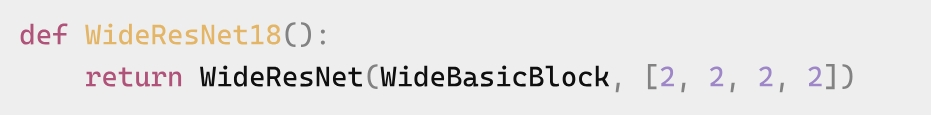
\includegraphics[width=0.48\textwidth]{wide_resnet18.png}
        \caption{WideResNet18 function}
        \label{fig:wide_resnet18}
    \end{figure}

    \subsection{Model Training and Evaluation}
    To evaluate the performance of the model, we first use the raw dataset without data augmentation to evaluate its performance. We use this model to train 100 epochs while calculating its test accuracy and loss rate. The detailed training plan is as follows:

    \subsubsection{Model Training:}
        
        The model is trained using the training dataset without data augmentation. The training process involves feeding the input data through the model, calculating the loss using a loss function (such as cross-entropy loss), and updating the model parameters using an optimizer (such as stochastic gradient descent, SGD). The model is trained for a fixed number of epochs (e.g., 100 epochs) or until the loss converges.
        
        we also specifies hyperparameters such as batch size, network depth, widening factor, number of classes, and number of epochs to a reasonable value, shown in figure \ref{fig:hyperparameter2}.

        \begin{figure}[ht]
            \centering
            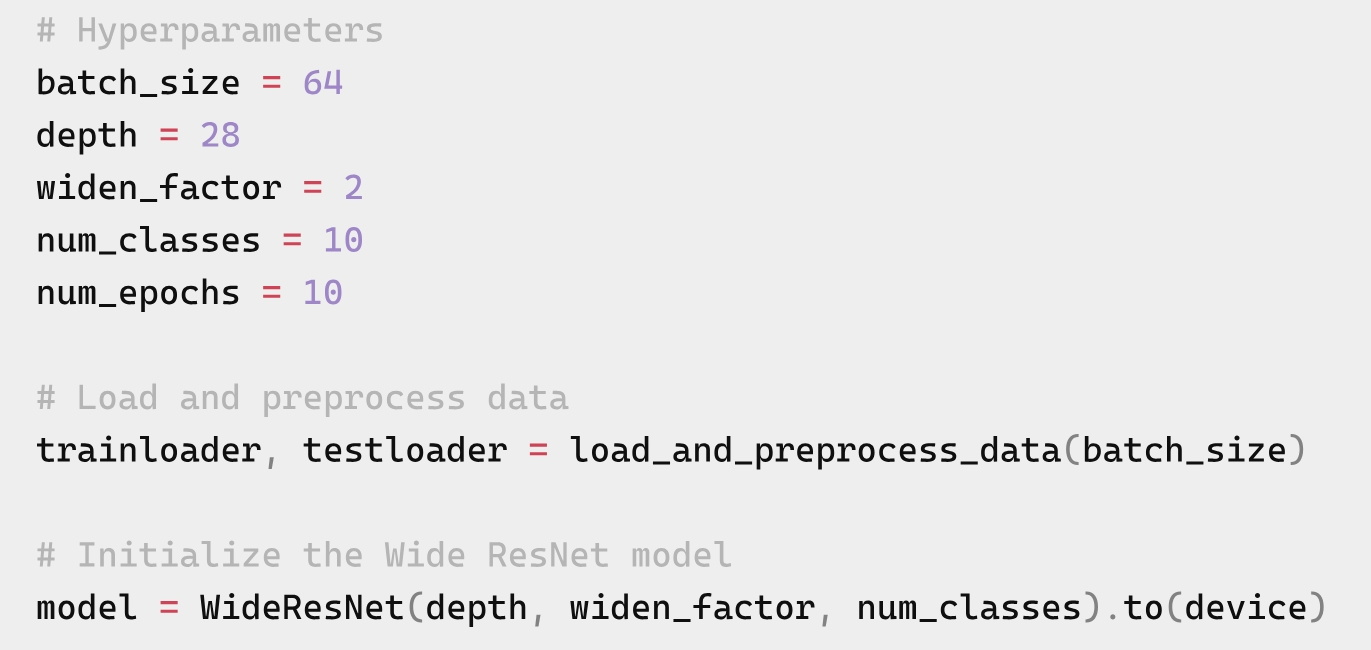
\includegraphics[width=0.48\textwidth]{hyperparameter2.png}
            \caption{Hyperparameters for training the model}
            \label{fig:hyperparameter2}
        \end{figure}

        \begin{itemize}
            \item Inputs:
            \begin{itemize}
                \item `model`': The WideResNet model.
                \item `trainloader`': DataLoader for the training set.
                \item `criterion`: The loss function (CrossEntropyLoss).
                \item `optimizer`: Adam optimizer.
                \item `device`: The device for training (CPU or GPU).
            \end{itemize} 
            \item Training Loop:
            \begin{itemize}
                \item Sets the model in training mode.
                \item Iterates through the batches in the training loader.
                \item Moves input data and labels to the specified device (CPU or GPU).
                \item Zeroes the gradients (`optimizer.zero\_grad()`).
                \item Performs forward pass, computes the loss, and backward pass for gradient computation.
                \item Updates the model parameters using the optimizer.
                \item Tracks and prints the running loss using tqdm for visual feedback.
            \end{itemize}
        \end{itemize}

    \subsubsection{Model Evaluation:} 
        
        After training the model, it is evaluated using the test dataset. The model's performance is evaluated using metrics such as accuracy, precision, recall, and F1 score. The model's performance is also visualized using a confusion matrix to show the distribution of predicted and actual labels.

        
        \begin{figure}[ht]
            \centering
            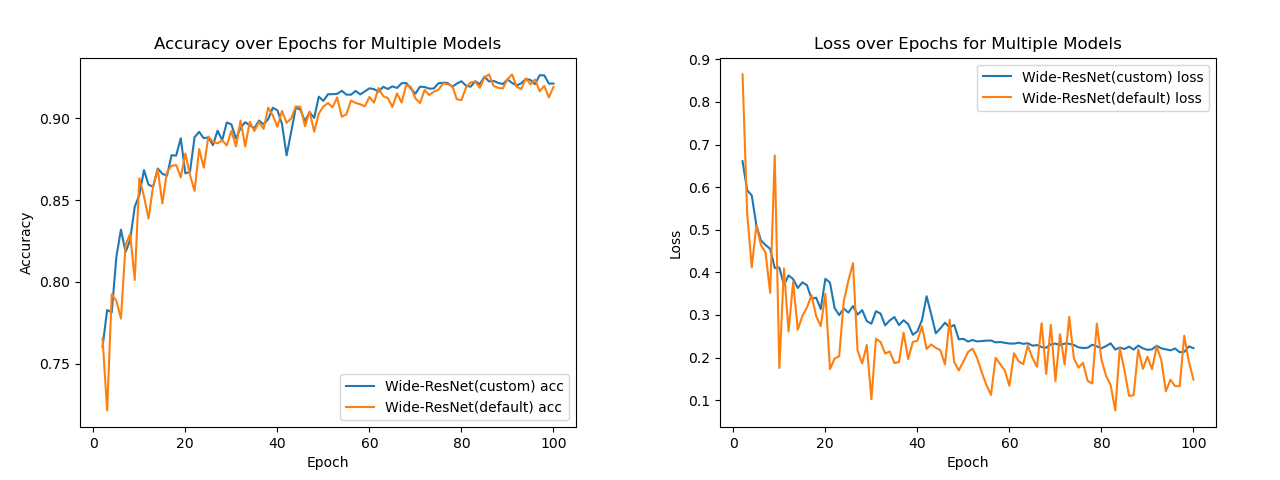
\includegraphics[width=0.48\textwidth]{Comparison With Default Wide-ResNet Model1.png}
            \caption{Comparison With Default Wide-ResNet Model1}
            \label{fig:Comparison With Default Wide-ResNet Model1}

            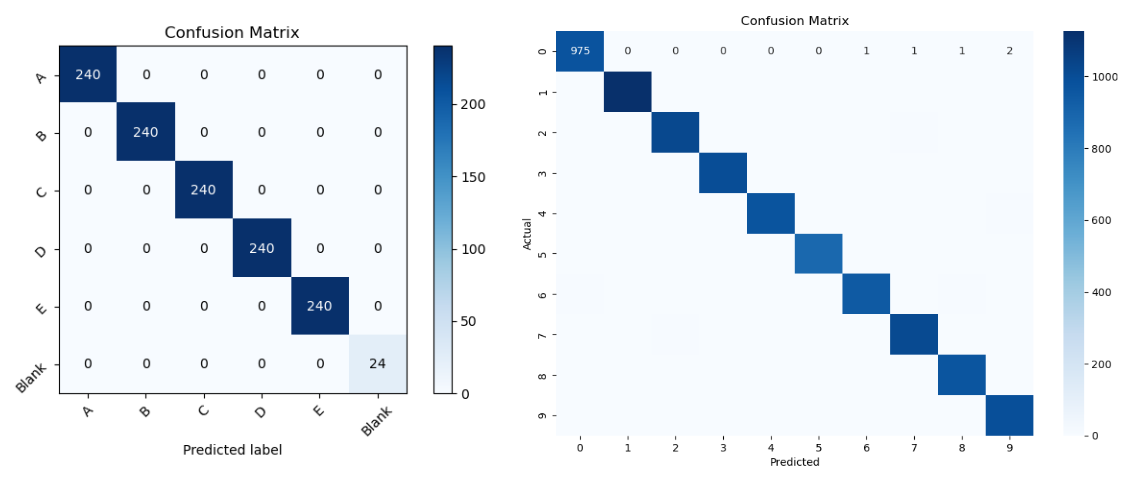
\includegraphics[width=0.48\textwidth]{conf_matrix1.png}
            \caption{Confusion matrix of answer and ID recognition} 
            \label{fig:conf_matrix1}

        \end{figure}

        From the results, it can be seen that the self-made Wide ResNet model achieved better results compared to the default model included in `torchvision`. The optimization of this model relative to the default model is mainly reflected in the following points:

        \textbf{Width factor of `Wide Basic Block`:}
        One of the core ideas of Wide ResNet is to improve performance by increasing the width (number of channels) of residual blocks. In the given code, the width factor is set to 4. This is a common value, but wider than the default value. Meanwhile, the initial convolutional layer `self.conv`1 increases the number of input channels from 1 (grayscale image) to 64. This can provide better performance when processing datasets.

        \textbf{Input size for fully connected layers:}
        The input size of the final fully connected layer `self.fc` is set to 256 * block. expansion * 4, where block. expansion is the extension factor defined in the `WideBasicBlock` class. Compared to the default model, our model has a larger fully connected layer that can provide larger inputs.

        \textbf{Adaptive average pooling layer:}
        In the default Wide ResNet, a global average pooling layer is usually used to convert the feature map of the last layer into a vector, and here an adaptive average pooling layer `nn.AdaptiveAvgPool2d (1,1)` is used, which can adapt to different input sizes.

    \subsection{Optimization and Hyperparameter Tuning}
    Currently, ResNet and CNN has achieved good classification results. However, in previous experiments, we did not perform data augmentation, using schedulers and optimizers. At the same time, no hyperparameter adjustments were made. Therefore, in this section, we will focus on testing the effects of different modules after addition.

    This experiment will use the standard CNN model to train 50 epochs with and without data augmentation, and plot their fitting curves. This is because in Chapter 4.3.2, the CNN model has a faster fitting speed and a more stable accuracy, while compared to ResNet model, although ResNet can achieve more satisfactory accuracy, it requires a much longer training time (about 2-3 hours per training session). Under controlled variables, the CNN model can also complete subsequent module experiments. The CNN model we use has 4 convolutional layers, two pooling layers, and two fully connected layers.

    \subsubsection{Data Augmentation:} Common data augmentation techniques include random rotation, flipping, scaling, and cropping. In this project, we use the torchvision.transforms module in PyTorch to apply data augmentation to the training dataset. The data augmentation techniques used include random flipping, random cropping. The data augmentation is applied to the training dataset but not the test dataset to ensure that the model is evaluated on the original data.
    
    \begin{figure}[ht]
        \centering
        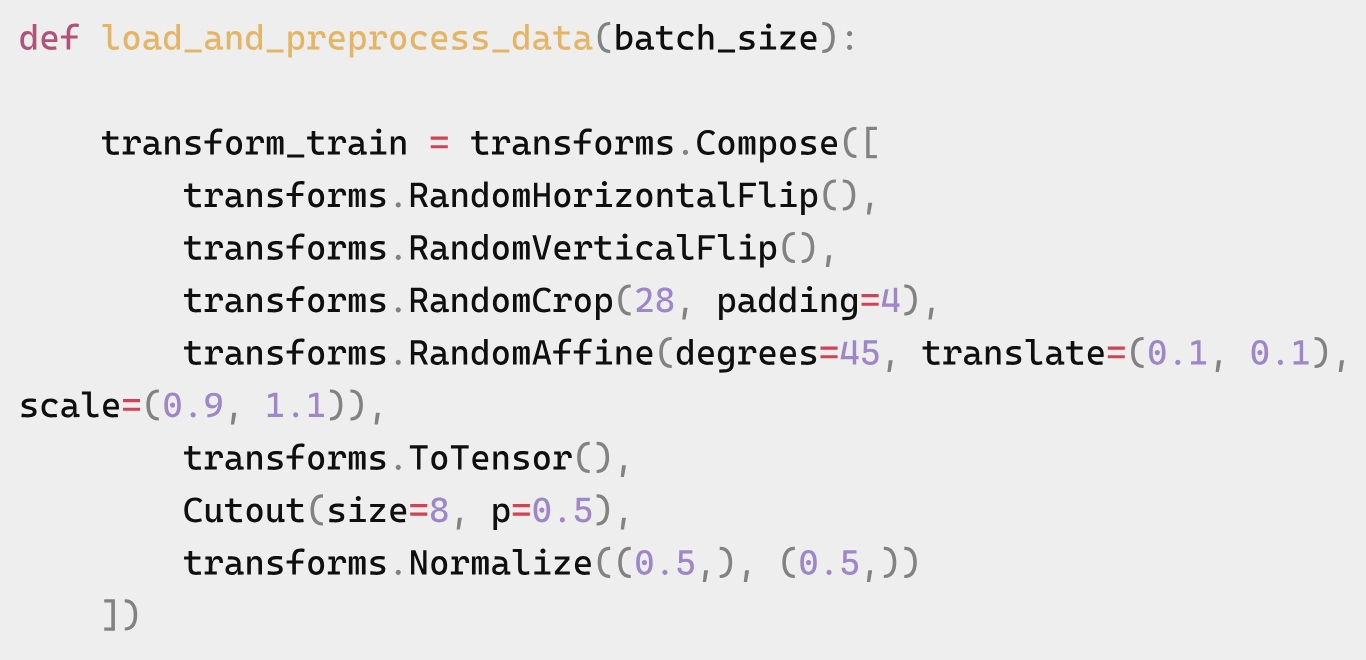
\includegraphics[width=0.48\textwidth]{transform.png}
        \caption{Implement data argumentation}
        \label{fig:transform}
    \end{figure}

    From the results, it can be seen that data augmentation significantly improves the fitting speed of the CNN model and shortens its training time. Meanwhile, its accuracy is higher compared to models without data augmentation. This is because data augmentation helps to increase the diversity of the training data and reduce overfitting, resulting in better generalization performance.

    \begin{figure}[ht]
        \centering
        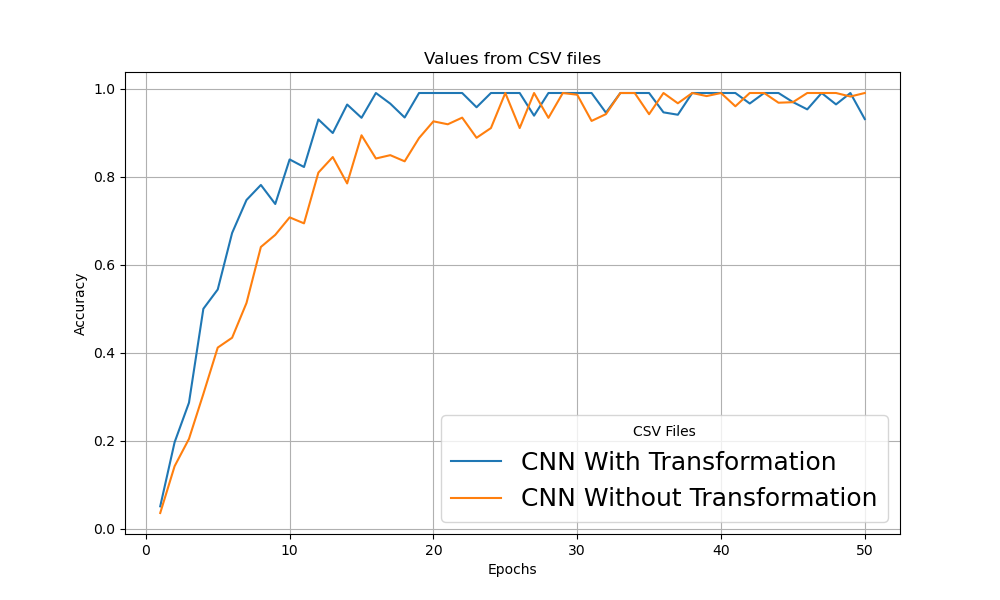
\includegraphics[width=0.48\textwidth]{data_argumentation.png}
        \caption{Result of data argumentation}
        \label{fig:data_argumentation}
    \end{figure}

    \subsubsection{Hyperparameter Tuning:} Hyperparameters are parameters that are set before the model is trained and can affect the model's performance. Common hyperparameters include the learning rate, batch size, number of epochs, and optimizer. Hyperparameter tuning involves finding the optimal values for these parameters to improve the model's performance. Techniques such as grid search, random search, and Bayesian optimization can be used to tune hyperparameters.

    This experiment will use hyperparameter grid search to match the optimal hyperparameter interval. Including parameters such as learning rate, optimizer, optimizer momentum, number of filters, dropout rate, etc. The hyperparameter search will be carried out multiple times, and each time the range of the most suitable hyperparameters will be gradually narrowed until the best hyperparameter combination is found. 
    
    To perform grid search, we use the GridSearchCV() function from sklearn.model\_selection. The parameter grid param\_grid is defined. The first search had 1728 different combinations.

    \begin{figure}[ht]
        \centering
        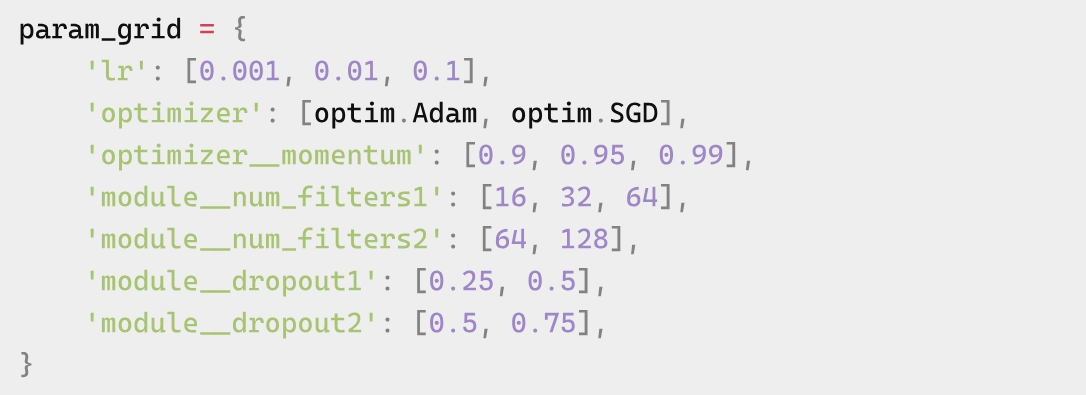
\includegraphics[width=0.48\textwidth]{grid_search.png}
        \caption{Hyperparameter grid search}
        \label{fig:grid_search}
    \end{figure}

    The results of the hyperparameter tuning experiment show that the optimal hyperparameters for the CNN model are a learning rate of 0.001, an optimizer of SGD, a batch size of 32, and a dropout rate of 0.5. These hyperparameters help to improve the model's performance and convergence speed. The results of the hyperparameter grid search are shown in the following figure.

    \begin{figure}[ht]
        \centering
        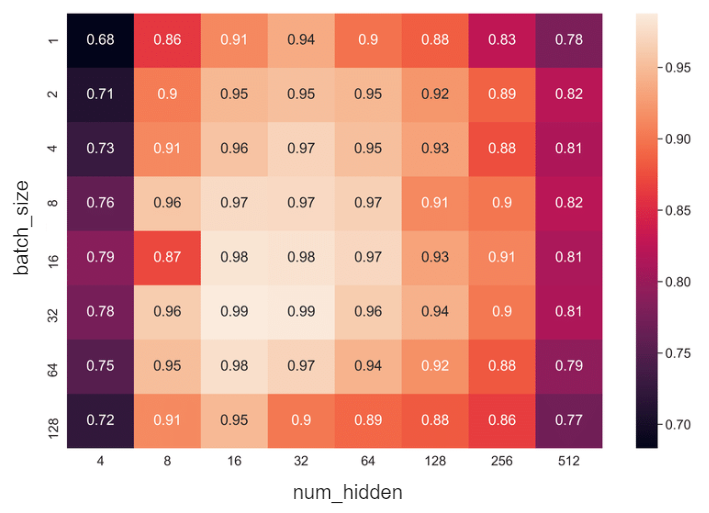
\includegraphics[width=0.48\textwidth]{grid_heatmap.png}
        \caption{Result of hyperparameter grid search}
        \label{fig:grid_heatmap}
    \end{figure}

    \begin{table}[ht]
        \begin{tabular}{|l|l|l|l|l|l|}
        \hline
        Lr & Optim & Batch Size & Drop & Acc & Loss \\ \hline
        0.001 & SGD & 32 & 0.5 & 0.989 & 0.06 \\ \hline
        \end{tabular}
        \caption{Optimal hyperparameters for the model}
        \label{tab:hyperparameters}
    \end{table}


    \subsubsection{SAM (Sharpness Aware Minimization) Optimizer}

    Sharpness Aware Minimization(SAM) is an optimization algorithm aimed at improving the generalization performance of neural network models. It was proposed by Liu et al\cite{foret2021sharpnessaware}. of Microsoft Research Asia in 2020. The design inspiration for SAM comes from an observation that there is a close relationship between the sharpness of model parameters and generalization errors in optimization problems.
    
    \begin{figure}[ht]
        \centering
        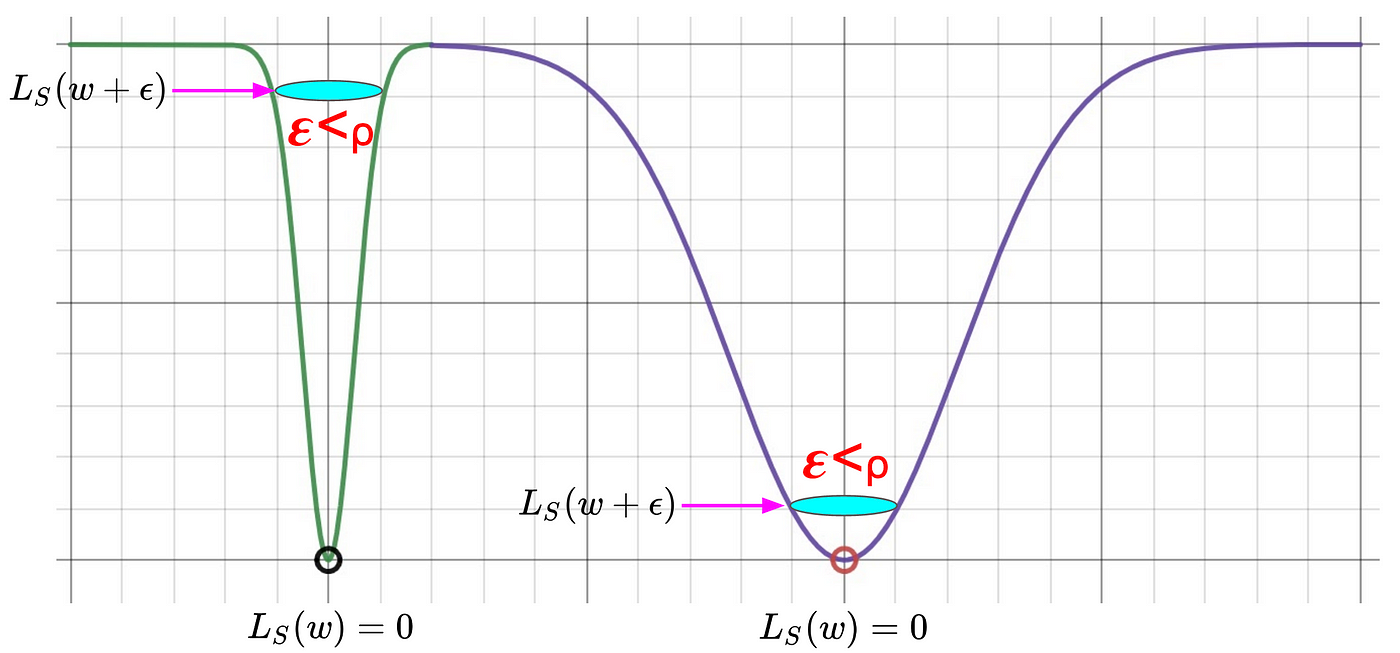
\includegraphics[width=0.48\textwidth]{SAM.png}
        \caption{Demostration of Sharpness Aware Minimization}
        \label{fig:SAM}
    \end{figure}

    Sharpness refers to the curvature of the loss function in the parameter space. During the training process, SAM attempts to minimize the loss function and update the parameters in the direction of smaller curvature. This process helps to avoid getting stuck in local minima in the parameter space, thereby improving the generalization performance of the model\cite{pmlr-v162-andriushchenko22a}. The core idea of SAM includes two steps:

    \begin {itemize}
        \item \textbf{1. Sharpness estimation of gradients:} 
        
        In each training step, SAM estimates sharpness by calculating the second derivative of the loss function with respect to the parameter. This sharpness estimate is called "sharpness" and represents information about the curvature of the loss function.

        \item \textbf{2. Sharpness aware update:} 
        
        SAM uses additional sharpness information in gradient updates to consider sharpness by adjusting gradients. This adjustment helps guide the gradient towards the direction with smaller curvature, thus better exploring the parameter space.
    \end {itemize}

    At the same time, we observed that those who used the SAM optimizer achieved good classification results, which made us hope to use it to optimize the model. The SAM code implementation for this project comes from GitHub user D. Samuel\cite{githubGitHubDavda54sam}. Full code will be included in the appendix.

    \begin{figure}[ht]
        \centering
        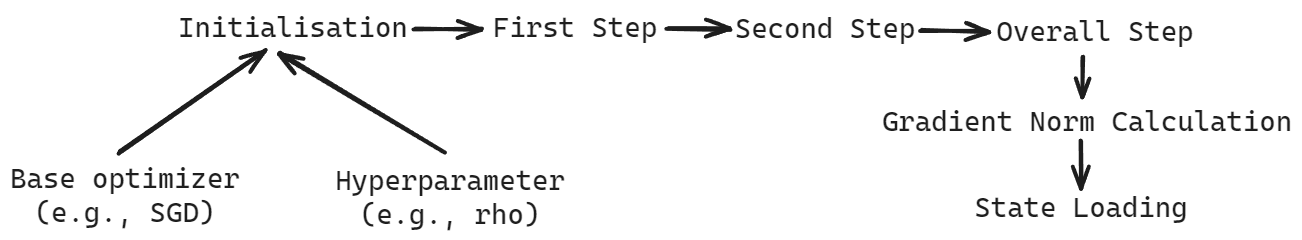
\includegraphics[width=0.48\textwidth]{sam_process.png}
        \caption{The process of SAM optimizer}
        \label{fig:sam_process}
    \end{figure}

    The SAM optimizer performs a two-step update, where the first step scales the parameters based on the gradient norm and an adaptive factor, and the second step reverts the parameters to their original values before applying the optimization step using the base optimizer. The adaptive scaling factor allows SAM to adapt the step size based on the sharpness of the loss landscape. Due to the need to pass in two parameters, the `train` function needs to be modified accordingly. In order to better compare the optimization capabilities that the SAM optimizer brings to the model, we will conduct a series of experiments to compare it with the baseline SGD optimizer.

    \begin{figure}[ht]
        \centering
        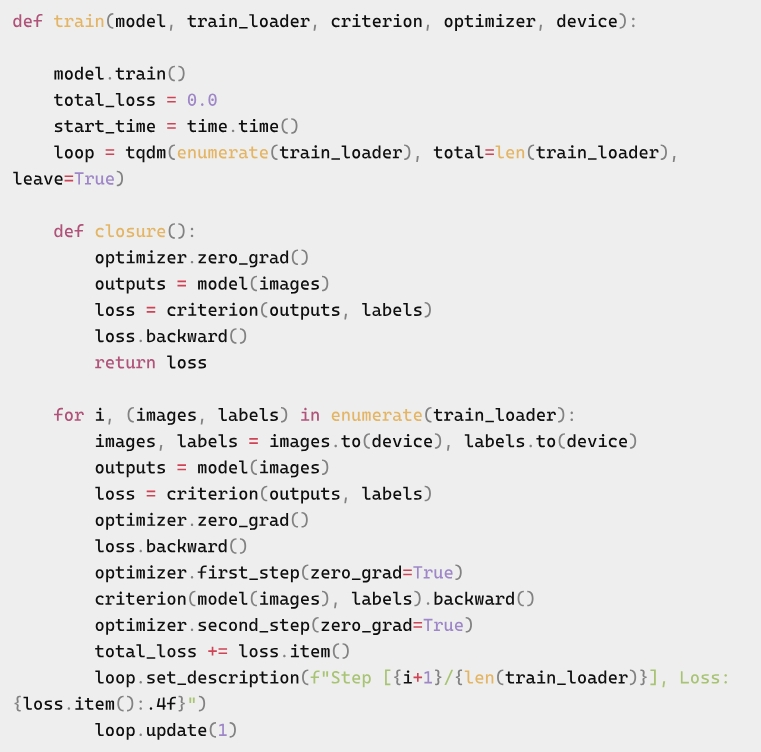
\includegraphics[width=0.48\textwidth]{train_function.png}
        \caption{Train function for the model using SAM optimizer}
        \label{fig:train_function}
    \end{figure}

    \textbf{Baseline Model with SGD:} The baseline model uses the SGD optimizer\cite{bottou_stochastic_2012} with a learning rate of 0.001 and a momentum of 0.9. The model is trained for 200 epochs with a batch size of 32. The model is evaluated using the test dataset to calculate the accuracy and loss, record metrics such as training accuracy, validation accuracy, and training time.
    
    \textbf{Model with SAM Optimizer:} The model with the SAM optimizer uses the same hyperparameters as the baseline model.(200 epochs with a batch size of 32). The model is evaluated using the test dataset to calculate the accuracy and loss, record metrics such as training accuracy, validation accuracy, and training time.

    \textbf{Comparison of Results:} The results of the baseline model and the model with the SAM optimizer are compared to evaluate the impact of the SAM optimizer on the model's performance,calculate the final accuracy achieved by both optimizers on the validation set.The results are visualized using plots to show the differences between the two models.

    \begin{figure}[ht]
        \centering
        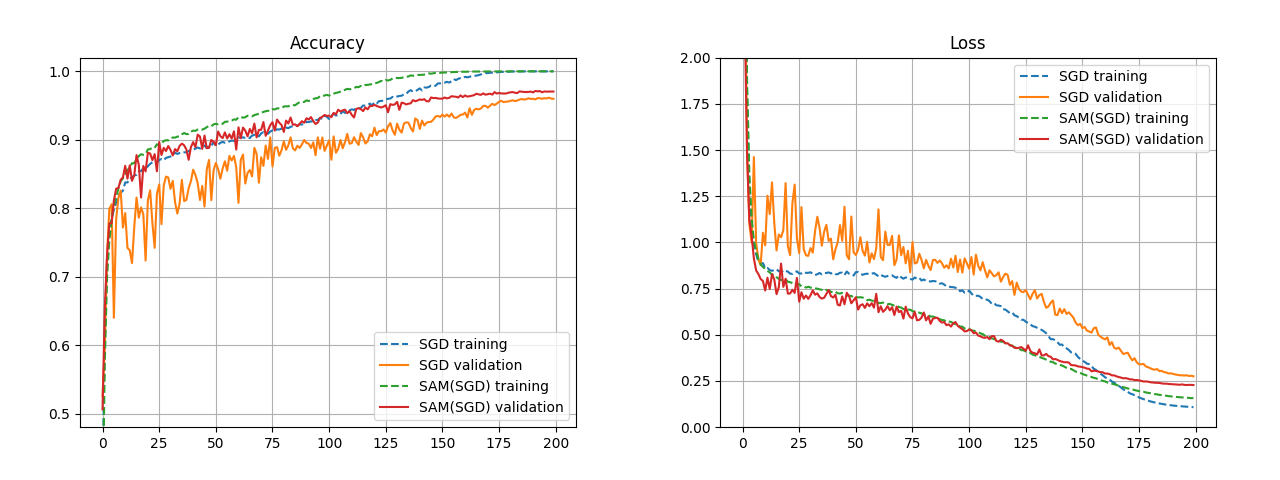
\includegraphics[width=0.48\textwidth]{Accuracy and Loss on Different Optimizers.png}
        \caption{Accuracy and Loss on Different Optimizers}
        \label{fig:Accuracy and Loss on Different Optimizers}
    \end{figure}

    From the experimental results, it can be seen that the addition of the SAM optimizer can significantly improve the performance of the model, with an accuracy improvement of approximately 1\%, reaching 99.8\%, while significantly reducing the loss rate. We believe that the Sharpness Aware Minimization (SAM) optimizer has some advantages over traditional SGD (Stochastic Gradient Descent) optimizers, especially in improving model generalization performance. The sharpness aware update strategy helps to avoid overfitting of the model to training data and improve its generalization ability to unseen data.

    At the same time, we have also noticed some negative impacts, especially in terms of computing resources. SAM requires two passes of parameters, which significantly reduces the training speed of the model, making it difficult for us to complete more tests within a limited time.

    \subsubsection{Learning Rate Scheduler} 
    
    Learning rate is an important hyperparameter in optimization algorithms, which controls the update amplitude of model parameters in each iteration. The purpose of a learning rate scheduler is to dynamically adjust the value of the learning rate to optimize the performance of the model.

    \begin{figure}[ht]
        \centering
        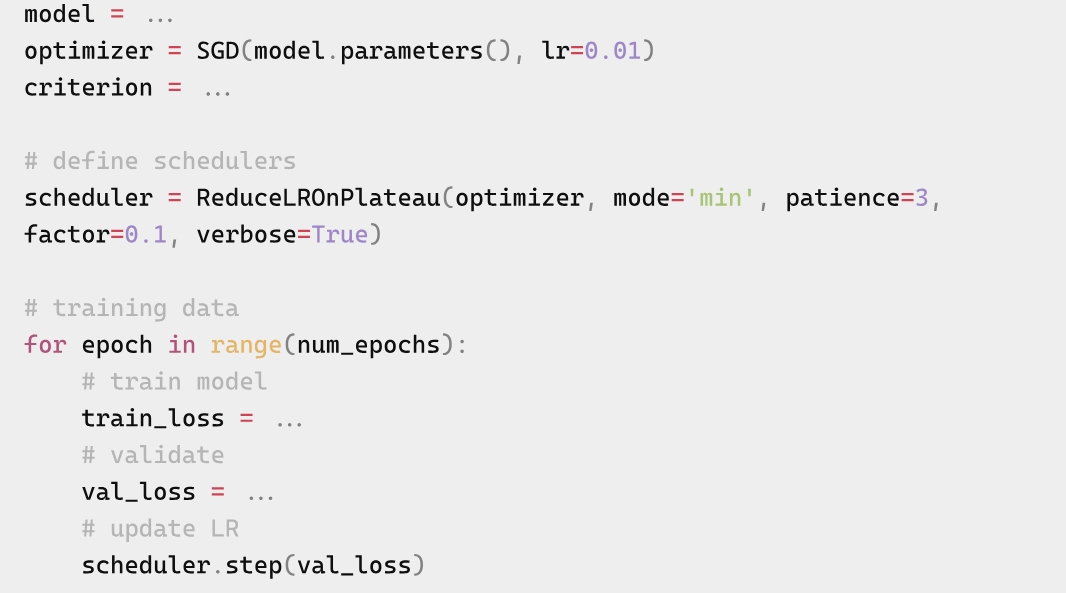
\includegraphics[width=0.48\textwidth]{scheduler.png}
        \caption{ReduceLROnPlateau scheduler}
        \label{fig:scheduler}
    \end{figure}


    The working principle of a learning rate scheduler is to gradually reduce the size of the learning rate during the training process. Such adjustments are usually based on the number of epochs of training or other indicators that measure training progress. Adjusting the learning rate appropriately can make the model converge to the optimal solution more stably, preventing excessive learning rate from causing the model to jump in the parameter space. Meanwhile, by dynamically adjusting the learning rate, the model is more likely to avoid getting stuck in local minima, thereby improving generalization performance on unseen data. We will test the impact of the `ReduceLROnPlateau` scheduler on model performance.

    The `ReduceLROnPlateau` scheduler is used to reduce the learning rate when a metric has stopped improving. The scheduler monitors the validation loss and reduces the learning rate by a factor of 0.1 when the loss has stopped improving for a certain number of epochs. Its core idea is to monitor the performance on the validation set and reduce the learning rate when performance stagnates, thereby fine-tuning the model parameters and improving training effectiveness. The scheduler is implemented using the `torch.optim.lr\_scheduler.ReduceLROnPlateau` class in PyTorch.

    An experiment should be conducted to test the impact of the ReduceLROnPlateau scheduler on model performance. For this, we will still use the CNN model for validation, running a total of two training sessions, one of which will not use any scheduler as a reference. The models, optimizers, loss functions, and learning rate schedulers are defined in figure \ref{fig:scheduler_train}.

    \begin{figure}
        \centering
        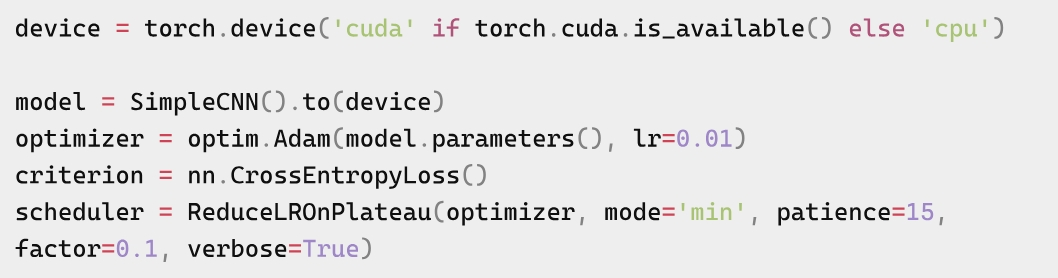
\includegraphics[width=0.48\textwidth]{scheduler_train.png}
        \caption{Training parameters with scheduler}
        \label{fig:scheduler_train}
    \end{figure}

    From the experimental results, it can be seen that the scheduler can provide a positive boost to model performance, but its impact does not seem to be as significant as other optimization methods. In terms of result testing, the two models achieved an accuracy of about 97.8\%, and the loss rate was controlled at around 0.2. We speculate that there may be several reasons for this:

    \begin{itemize}
        \item \textbf{Improper selection of scheduler parameters:} 
        
        The performance of a learning rate scheduler largely depends on the selection of parameters. For example, the patient parameter represents the number of tolerance rounds for performance stagnation, and the factor parameter represents the factor that reduces the learning rate. The values of these parameters need to be adjusted according to specific problems and models. Improper parameter selection may result in the scheduler not being able to effectively adjust the learning rate.
        
        \item \textbf{Overfitting or underfitting:} 
        
        If the model overfits or underfits on the training data, the learning rate scheduler may not be able to significantly improve performance. Overfitting may indicate that the model has achieved high accuracy on the training set, but has limited generalization ability on the validation set. Underfitting may indicate insufficient capacity of the model and require a more complex model structure.
        
        \item \textbf{Problem complexity:} 
        
        The dataset is relatively simple, and for certain models and problems, the advantage of learning rate schedulers may not be significant. On more complex tasks and datasets, the impact of a learning rate scheduler may be more significant.
        
    \end{itemize}

    
    \begin{figure}[h]
        \centering
        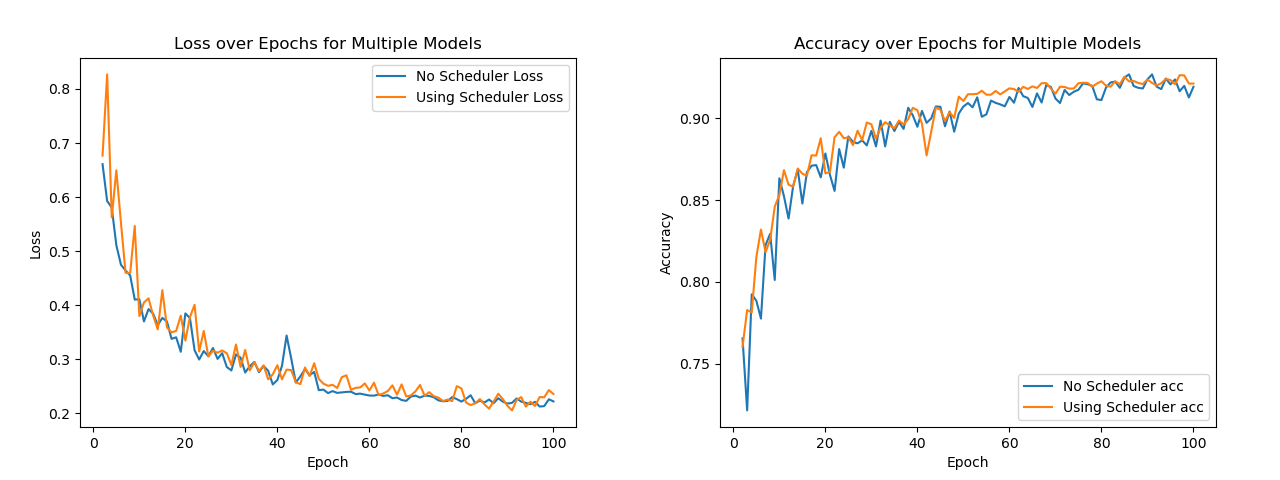
\includegraphics[width=0.48\textwidth]{Scheduler Optimization Result.png}
        \caption{Scheduler Optimization Result}
        \label{fig:scheduler_result}
    \end{figure}

    At the same time, we also noticed that the `patient` parameter of `ReduceLROnPlateau` has a significant impact on the training results of the model,shown in figure \ref{fig:patience}. When the `patient` parameter is set to 10, the model can achieve a higher accuracy, while the loss rate is also lower. This indicates that the `patient` parameter is an important factor in determining the performance of the learning rate scheduler.

    The `patient` parameter determines how many rounds of performance stagnation will trigger the adjustment of the learning rate. A smaller patient value means more frequent learning rate adjustments, while a larger value means fewer adjustments. This will affect the dynamic changes in the learning rate of the model throughout the entire training process.

    A smaller `patient` may cause the model to be overly sensitive to small fluctuations in performance, triggering a reduction in learning rate in a shorter period of time. On the contrary, a larger patient may cause the model to maintain a longer learning rate even when performance is stagnant.

    \begin{figure}[h]
        \centering
        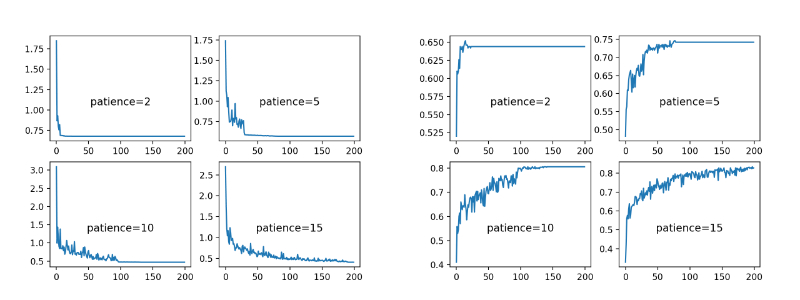
\includegraphics[width=0.48\textwidth]{patience.jpeg}
        \caption{Impact of the `patient` parameter on model performance}
        \label{fig:patience}
    \end{figure}
    
    \subsection{Automatic Grading and Output}

    After the model training and optimization process, the next step is to integrate automatic grading and student ID recognition modules into the system. The grading program will take the model prediction result as input, compare with master answer and generate the final output. The output will include the student ID, the answers to each question, and the final score in a DataFrame. This service consists of three python backend programs: `get\_master\_answer.py`, `validation.py`, and `ans\_eval.py`.

        \subsubsection{Obtaining Master Answer}
        As mentioned in the previous article, users have two ways to upload standard answers: upload a csv file or upload a pdf file. These two upload methods need to be run by two different systems, especially the part responsible for uploading and processing PDF files. This is the most important function of the get\_master\_answer program.

        The get\_master\_answer program is responsible for extracting the master answer from the uploaded PDF file. The program also uses the PyMuPDF library\cite{pymupdf} to extract answers from the PDF file and then processes the image to obtain the master answer. 

        \begin{figure}[ht]
            \centering
            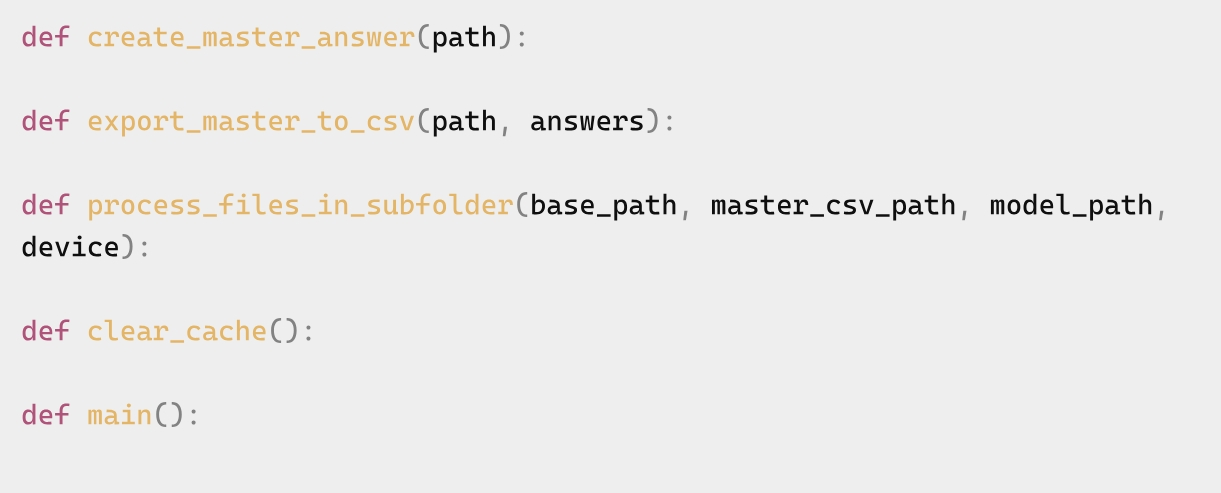
\includegraphics[width=0.48\textwidth]{get_master_answer.png}
            \caption{Overview of the functions in get master answer program}
            \label{fig:get_master_answer}
        \end{figure}

        The answer files uploaded by users will go through the same cropping process and be handed over to the neural network for recognition. The identified result will be used as the standard answer. But unlike the ordinary recognition mode, there is no need to grade the standard answer, nor does it need to recognize the student ID on the PDF file. This means that the model needs to store the recognition results immediately after the recognition is completed, rather than passing them to the grading service. At the same time, considering that the model may be wrong in identifying standard answers, the identification results need to be confirmed by the user before they can be used for grading. Therefore, after the identification is completed, the program also needs to initiate an HTTP download request to transmit the identified answer from the server to the user's computer for user confirmation. After the recognition is completed, the program will clear the cache and delete the answer sheet images stored on the server. The program will store the identification results in a CSV file on both server (csv/master\_answers) and user's device for later use. If the user chooses not to modify the answer file, the analysis can begin directly with the answer file stored on the server. For users who upload csv files directly, the software does not need to go through the identification process, so the file is directly passed to the folder used to store standard answers on the backend (csv/master\_answers).

        This CSV file consists of 4 columns, including numbers, answers, weights, and parts. Weight refers to the score of each question, which can be modied for customization. The default score is 1. Part refers to the sections of the test paper that different questions belong to. The default number of questions is 120, user can also delete unnecessary rows directly. The software will automatically recognize the number of questions using get\_num\_questions function by counting the number of rows in master answer csv file during processing.

        \begin{figure}[ht]
            \centering
            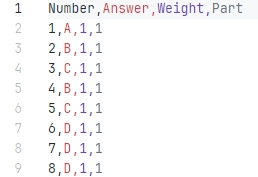
\includegraphics[width=0.3\textwidth]{master_ans_csv.png}
            \caption{The structure of the master answer CSV file}
            \label{fig:master_ans_csv}
        \end{figure}


        \subsubsection{Validation}

        The function of the validation program is to predict the student ID and answer of the answer sheet through the model. This program is only responsible for predictiong answers but not grading. The output content is two lists, containing the prediction results of all the students' answers and IDs respectively. In the previous chapters, we introduced how to train and optimize neural network models, and the program needs to load the trained model file and switch to inference mode. It mainly consists of 4 functions, including `load\_model`, `predict\_image`, `get\_id`, and `get\_answers`.

        \begin{itemize}
            \item \textbf{load\_model:} Load the trained model file and switch to inference mode.
            \item \textbf{predict\_image:} Predict the student ID and answer of the answer sheet.
            \item \textbf{get\_answers:} Use the model to infer the answer, assign the correct category name to the answer, and finally return a list containing all answers.
            \item \textbf{get\_id:} Same as answer inference function, extract the student ID from the answer sheet. Returns a list containing student IDs.
        \end{itemize}

        \begin{figure}[ht]
            \centering
            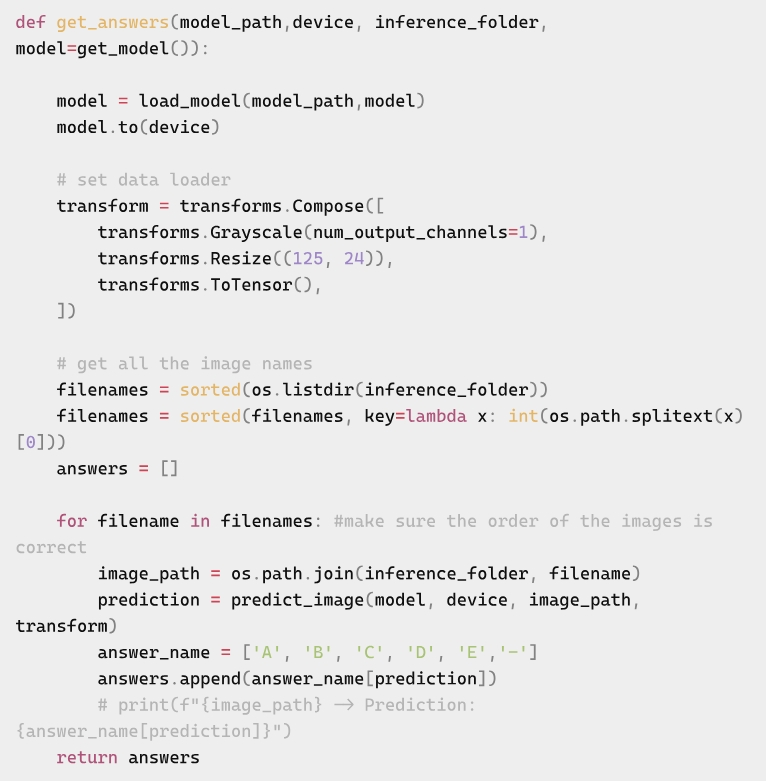
\includegraphics[width=0.48\textwidth]{get_ans_code.png}
            \caption{Code implementation of get\_answers function}
            \label{fig:get_ans_code}
        \end{figure}

        \subsubsection{Grading and Output}

        The ans\_eval program is responsible for comparing the student's answer with the master answer and generating the final score. The program will take the student's answer and the master answer as input, compare the two, and calculate the score based on the comparison results. The program will also generate a DataFrame containing the student ID, the answers to each question, and the final score. The DataFrame will be saved as a CSV file for later use.

        \textbf{Input Directories Setup:}

        This program expects two sets of input folder: one for student answer images (ans\_inference\_base\_folder) and another for student ID images (id\_inference\_base\_folder). It also needs a directory containing master answer files in CSV format (master\_answers\_folder).
        Each student's answer and ID images should be organized into subdirectories within these base folders.

        \textbf{Prepare Master Answer Files:}

        The function load\_master\_answers reads all CSV files in the master\_answers\_folder directory, these CSV files contain the master answers and weights for the questions, and each file corresponds to a different test.

        \textbf{Extract Student IDs and Answers:}

        The function get\_id and get\_answers are used to extract student IDs and answers from images. As mentioned, These functions use neural network models (ans\_model\_path and id\_model\_path) to process the images.

        \textbf{Evaluate Answers:}

        The function answer\_eval iterates over each master answer file to evaluate student responses for that specific test. This is the most important function in this program. It is responsible for scoring and organizing the data. Including calculating accuracy, scores, counting correct answers and wrong answers, calculating scores for each part of the test paper, etc. The calculated results will be uniformly stored in a DataFrame as the return value of the function, and another csv generating function will write the results to a csv file.

        For each student's subdirectory in the answer and ID base folders, the program extracts the student ID using get\_id and the answers using get\_answers. It then compares the student's answers with the master answers using `calculate\_part\_correct\_and\_total' and `format\_answers' function. calculate\_part\_correct\_and\_total' function is used to calculate the score for each paper section individually. `format\_answers' function is to format the provided answers for display purposes. It will display correct answers in capital letters, incorrect answers in lowercase, and unfilled answers in "-". After that, the ans\_eval function will calculate the total score for each student and generate a DataFrame containing the student ID, answers, and score, and store them in a CSV file using export\_result\_to\_csv function. When all work has been completed, the program will call the clear cache function to delete all the data just processed.

        \begin{figure}[ht]
            \centering
            \includegraphics*[width=0.48\textwidth]{ans_eval_structure.png}
            \caption{Structure of the ans\_eval program}
            \label{fig:ans_eval_structure}

            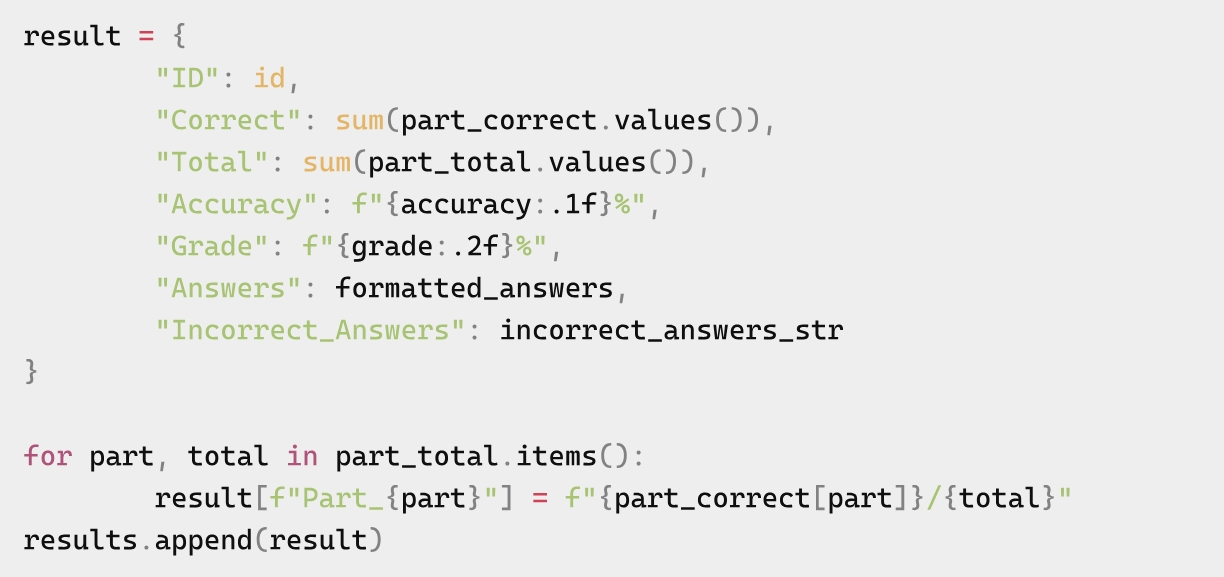
\includegraphics[width=0.48\textwidth]{result_dataframe.png}
            \caption{The code used to generate result DataFrame}
            \label{fig:result_dataframe}
        \end{figure}

        \subsection{Other Functional Implementation}

        \subsubsection{Email Notification}
        The email sending service is used to email student test scores to students. This program reads the generated student grade files and the student personal information files uploaded by the user, obtains the students' mailboxes, and sends emails to each student through the SMTP server. The program mainly consists of three parts:

        \begin{figure}[ht]
            \centering
            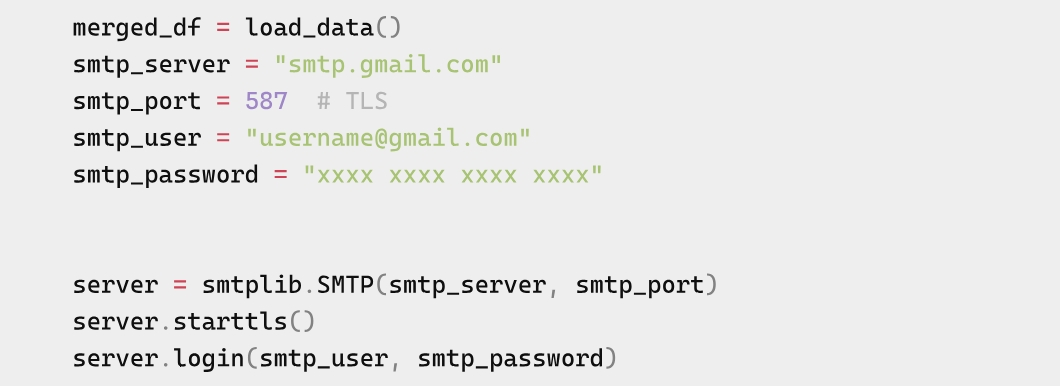
\includegraphics[width=0.48\textwidth]{smtp.png}
            \caption{Configure SMTP server}
            \label{fig:smtp}
        \end{figure}

        \begin{itemize}
            \item \textbf{Data loading:} The load\_data() function loads student information(A CSV file with 3 columns: Full\_Name, ID, Email\_Address) and test scores from CSV files in two directories. The two data sets are then merged via the ID field to create a dataframe containing student information and corresponding grades.
            \item \textbf{Email sending:} The send\_email() function iterates over each row in the merged dataframe and sends an email to each student containing their test score. The function sets up the configuration of the SMTP server and uses Python's smtplib library to send emails. The email content is constructed by MIMEText and contains the student's test scores and related information.
            \item \textbf{Main function:} The main function of the program loads the data, sends the emails, and prints a message indicating the completion of the email sending process.
            
        \end{itemize}
        
        \begin{figure}[ht]
            \centering
            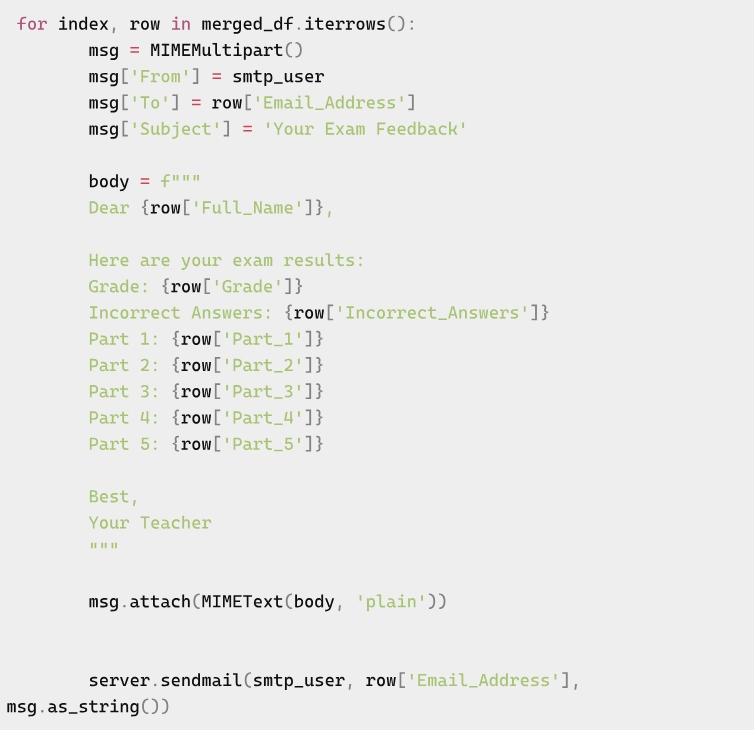
\includegraphics[width=0.48\textwidth]{email_content.png}
            \caption{The content of the email sent to students}
            \label{fig:email_content}
        \end{figure}

        \subsubsection{Score Visualization}
        The score visualization service is used to generate visualizations of student test scores. This program reads the generated student grade files and generates a bar chart showing the highest, lowest, mean and overall accuracy of test scores, and a pie chart showing the top 5 questions with highest error rate. The program mainly consists of the following parts:

        \begin{itemize}
            \item \textbf{Data loading:} The load\_student\_scores() function loads student test scores from a CSV file and creates a dataframe containing the scores. This function accepts a file path parameter student\_scores\_path.
            \item \textbf{Bar Chart function:} The bar\_chart() function generates a bar chart showing the highest, lowest, mean, and overall accuracy of test scores. 
            \item \textbf{Pie Chart function:} The pie\_chart() function generates a pie chart showing the top 5 questions with the highest error rate. It extract all incorrect answers (separated by ';') from the 'Incorrect\_Answers' column of the dataframe, Then use counter to count the number of times each incorrect answer appears. Find the 5 answers with the most errors, form labels and corresponding sizes (number of errors), and calculate the percentage of these errors.
            \item \textbf{Display:} These images will be stored in the static file folder on the backend of the webpage and sent to the frontend for display on the webpage.
        \end{itemize}

        \begin{figure}[ht]
            \centering
            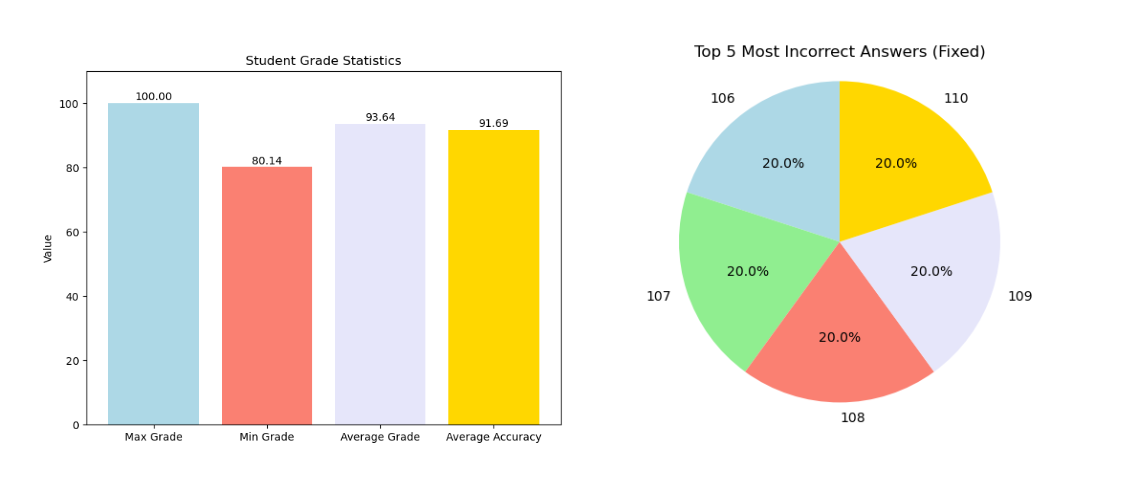
\includegraphics[width=0.48\textwidth]{score_visualize.png}
            \caption{An example of score visualization}
            \label{fig:score_visualize} 
        \end{figure}



        \subsection{Website Implementation}

        The website provides a user-friendly interface for users to interact with the system. The website consists of two pages, including the home page and result page. The home page provides an overview of the system and its features and allows users to upload answer sheets and master answer files. The result page displays the final grading results and allows users to view the results in CSV format.

        \subsubsection{Frontend Implementation}

        The frontend design of the website is implemented using HTML, CSS, and JavaScript. The website uses the Node.js framework for responsive design and styling. The home page contains a form for users to upload answer sheets and master answer files. The result page displays the final grading results in a tabular format and allows users to download the results in CSV format.

        \textbf{HTML:} 
        
        The HTML code defines the structure of the website, including the layout of the home page and result page. Among them, index.html is the html code of the homepage, and results.html is the code of the results page.

        \begin{figure}[ht]
            \centering
            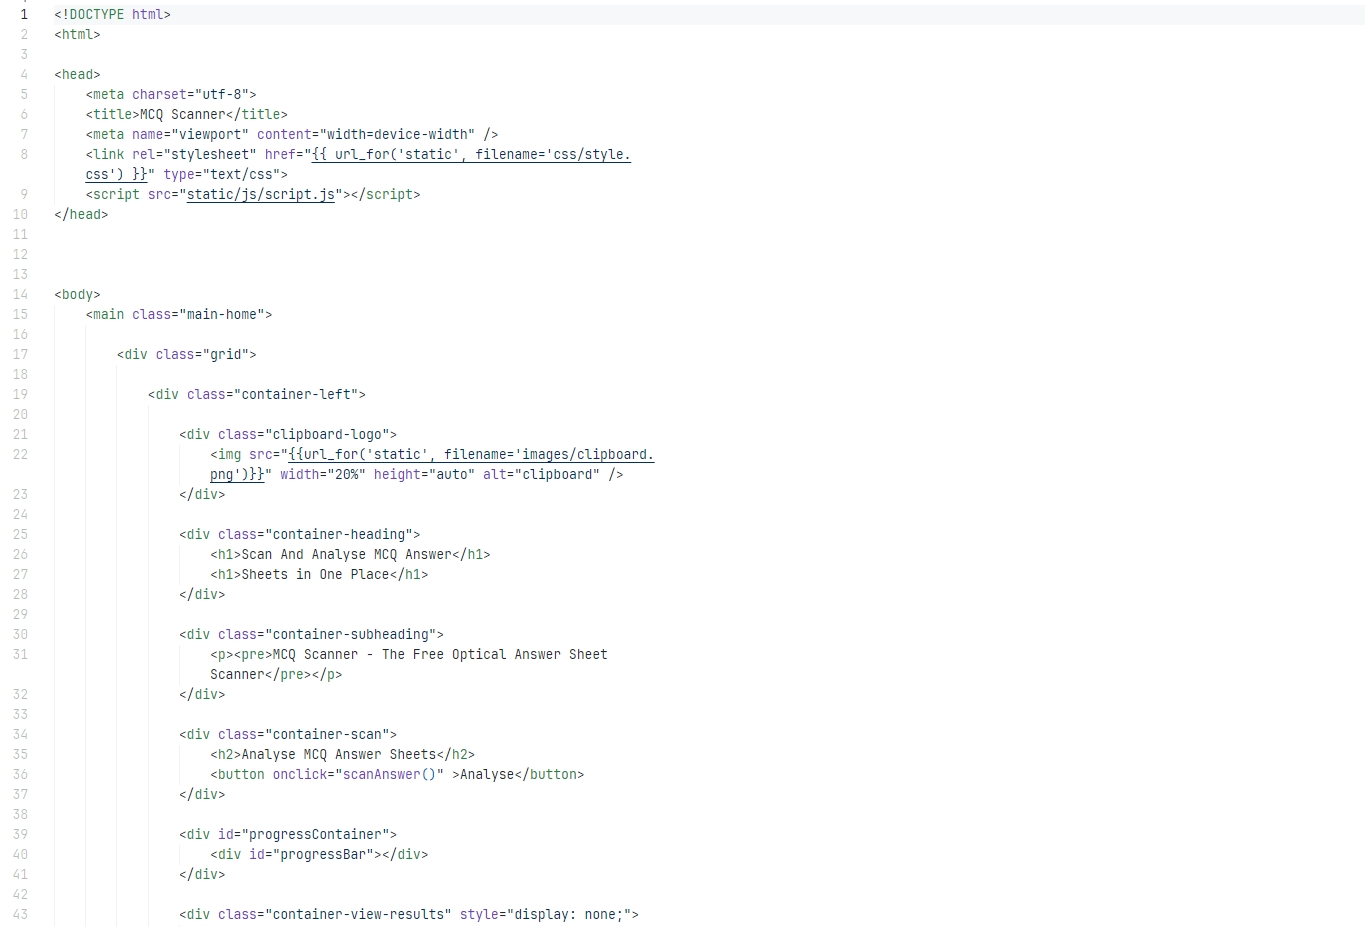
\includegraphics[width=0.48\textwidth]{html_preview.png}
            \caption{HTML code for the website}
            \label{fig:html_preview}
        \end{figure}

        \textbf{CSS:} 
        
        The CSS code styles the website, including the colors, fonts, and layout of the elements on the page. To ensure consistent styles, the homepage and results pages share a style.css file, which is stored in the static folder on the front end.
        
        \textbf{JavaScript:} 
        
        The JavaScript code adds interactivity to the website, such as form validation and file upload functionality. The JavaScript code also handles the display of the grading results on the result page. It contains a script.js file, and the two pages share this js code. It is stored in the static folder of the project. The Javascript part is mainly composed of following functions:

        \begin{itemize}
            \item \textbf{Upload and Preview File:} Upload the file to the server. The function uses the fetch API to send the file to the server and display a preview of the file on the page. The preview function is used to display the content of the uploaded PDF file on the page. The function uses the PDF.js library to render the PDF file on the page.
            \item \textbf{Upload CSV:} Upload CSV files to the server. The process of this function is exactly the same as uploading PDF, but the preview function is removed.
            \item \textbf{Upload Student Info:} Upload the student information csv file containing student email addresses to the server for sending emails. The process is similar to the previous two functions, but the endpoint is different.
            \item \textbf{Drag Over:} This part is used to implement the file drag and drop upload function. dragArea.addEventListener() adds an event listener, which is triggered when the user drags the file to the specified area and releases it. In this event listener, the default behavior (that is, the browser's default file dragging behavior) is first prevented, and then the previously added class name 'drag-over' is removed to restore the original style of the drag area. Next, get the dragged file and check whether its type is a PDF file. If not, a prompt box will pop up asking the user to drag the PDF file. If the file type is correct, use FormData to encapsulate the file and send the file to the server asynchronously through the fetch API. If the upload is successful, a prompt box will pop up. If the upload fails, an error message will be printed on the console.
            \item \textbf{Scan Answer:} Display a progress bar while scanning for answers, and to display the results after the scan is complete.At the same time, the data in JSON format returned by the server is processed.
            \item \textbf{showError:} Display an error message if there is an issue with the file upload.
            \item \textbf{hideError:} Hide the error message after the issue is resolved.
            \item \textbf{validateForm:} Validate the form before submitting the file.
            \item \textbf{showResult:} Display the grading results on the result page.
            \item \textbf{Send Email:} Send the grading results to students via POST. It transmits a request to the backend, and when the backend receives it, it runs the python code responsible for sending the email.
        \end{itemize}

        \begin{figure*}
            \centering
            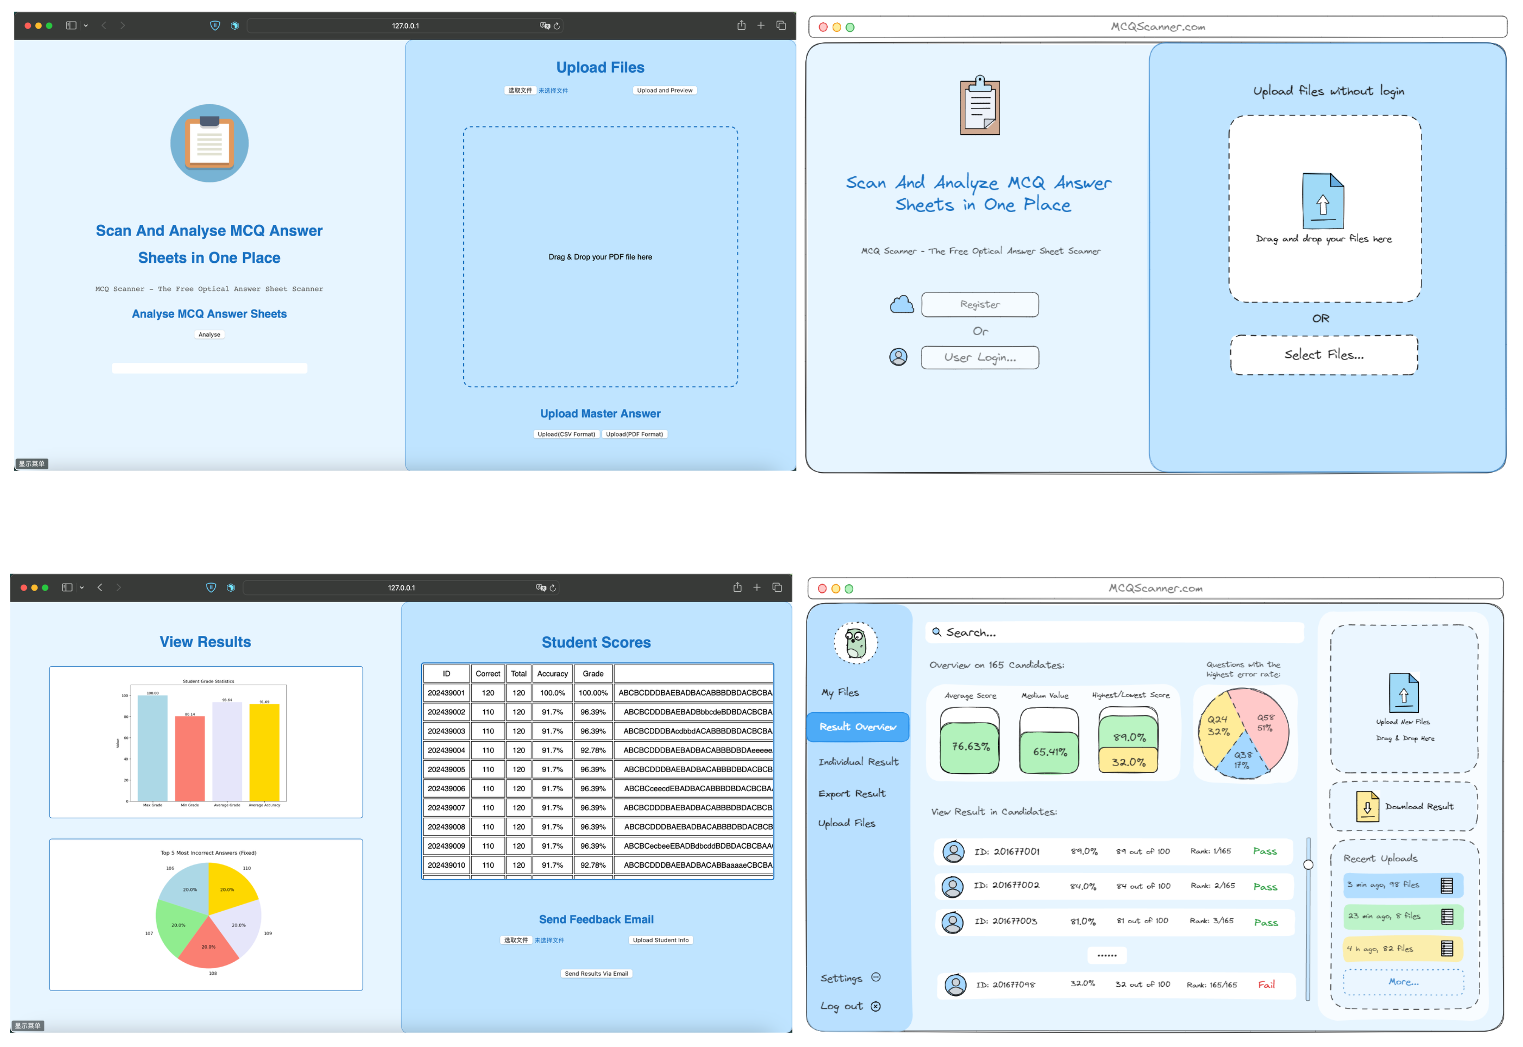
\includegraphics[width=0.9\textwidth]{ui_implementation.png}
            \caption{Webpage UI implementation compared to the design draft}
            \label{ui_implementation}
        \end{figure*}
        \subsubsection{User Interface Design}
        The user interface design of the website has been implemented as much as possible in the direction of restoring the design draft. The design of the homepage basically refers to the original design draft, but due to changes in functionality and in order to comply with ethical standards, the design of the results page has undergone major changes. Currently we only retain the most basic function of viewing overall score statistics, and have added a new function for sending emails on this page. Also to comply with ethical standards, users are not allowed to set their email here, but need to configure it in the send\_email.py file of the source code. The final implementation of the website is shown in the figure \ref{ui_implementation}.

        \subsubsection{Backend Framework}
        The backend of the website is implemented using Python Flask, which provides the server-side logic for handling file uploads, processing, and sending emails. The backend framework contains an app.py file, which contains multiple routes for implementing functions. The backend consists of the following parts:
        \begin{itemize}
            \item \textbf{Page Routing:} Including the routing of the home page and result page. Returns the corresponding HTML page when the user accesses the specified URL. When the user clicks to jump to the results page, the route responsible for returning to the results page will also start the background score visualization program and obtain two statistical charts containing student scores, which are then passed to the front end for display on the page.
            \item \textbf{File Upload:} The file upload function is responsible for receiving the uploaded PDF and CSV files from the front end and saving them to the server. The function uses the Flask request object to access the uploaded files and save them to the specified directory on the server. This part consists of four routes, which are responsible for uploading pdf files, uploading answer pdf, uploading answer csv files, and routes for uploading student information required when sending emails.
            \item \textbf{Answer Scanning:} The answer scanning function is responsible for processing the uploaded answer sheets and master answer files. The function consists of one route, for scanning the answer and sending the grading results to the front end. 
            \item \textbf{Email Sending:} The email sending function is responsible for sending the grading results to students via email. The function consists of one route, which sends the grading results to the specified email addresses.
            \item \textbf{File Download:} The file download function is responsible for allowing users to download the grading results in CSV format. The function consists of two routes, which allows users to download the grading results in CSV format, and download the master answer files in CSV format. When the user uploads the standard answer in pdf format, the backend will automatically analyze the answer and use this route to download the analysis results to the user's device.
            \item \textbf{Error Handling:} The error handling function is responsible for handling errors that occur during file uploads and processing. The function consists of one route, which returns an error message to the front end when an error occurs, including missing files, incorrect file types, and server errors.
        \end{itemize}


    

\section{Testing and Evaluation}

    \subsection{Model Performance}
    In Chapters 4.4 and 4.5, we have discussed model construction and model optimization in detail, which already involved some performance evaluation of the model. Therefore, this chapter will summarize the performance indicators of the Wide-ResNet18 model ultimately used in this project. The model is trained over 100 epochs. Most of the evaluations and charts used in this chapter are based on the answer recognition model. Since the ID recognition model uses a similar architecture and has less recognition content, the two models will be combined and discussed in this chapter.

    \subsubsection{Model Accuracy} 
    The accuracy of the model is an important indicator of its performance. It measures the proportion of correctly recognized answers to the total number of answers. The accuracy of the model is calculated as the number of correct predictions divided by the total number of predictions. The accuracy of the model is calculated using the following formula:

    \begin{equation}
        Accuracy = \frac{Number of Correct Predictions}{Total Number of Predictions}
    \end{equation}

    \begin{figure}[ht]
        \centering
        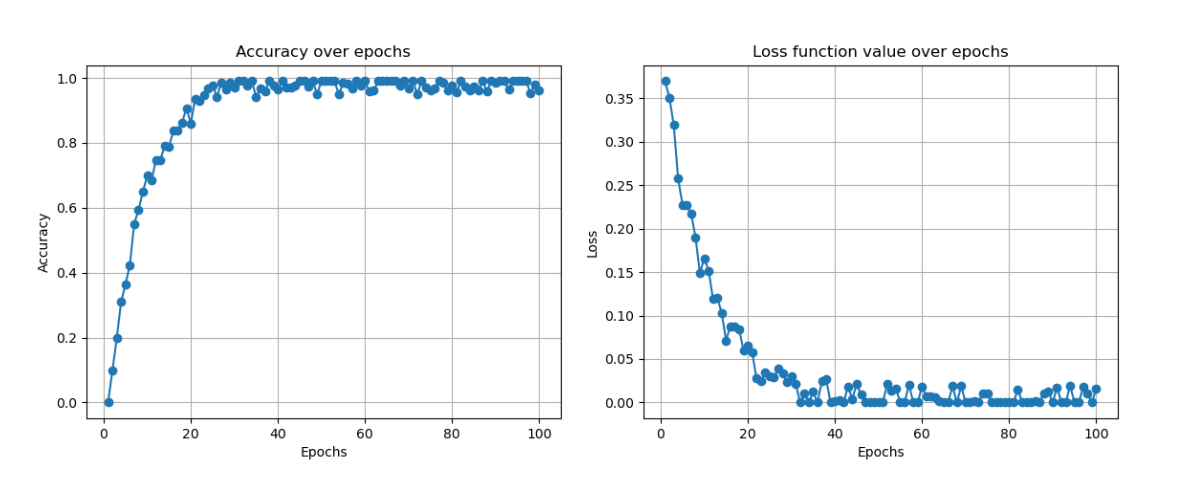
\includegraphics[width=0.48\textwidth]{loss_acc.png}
        \caption{Accuracy and loss curve of the model}
        \label{fig:acc_loss}
    \end{figure}

    Figure \ref*{fig:acc_loss} plots the fitting curve of the model along with the loss function. The model achieves an accuracy of 99.974\% on the validation set, which indicates that the model achieved high accuracy in recognizing answers.

    \subsubsection{Precision, Recall and F1 Score}
    Precision and recall are two important metrics for evaluating the performance of a classification model. Precision measures the proportion of correctly predicted positive samples to the total number of predicted positive samples. Recall measures the proportion of correctly predicted positive samples to the total number of actual positive samples. The precision and recall of the model are calculated using the following formulas:

    \begin{equation}
        Precision = \frac{True Positive}{True Positive + False Positive}
    \end{equation}

    \begin{equation}
        Recall = \frac{True Positive}{True Positive + False Negative}
    \end{equation}

    \begin{figure}[ht]
        \centering
        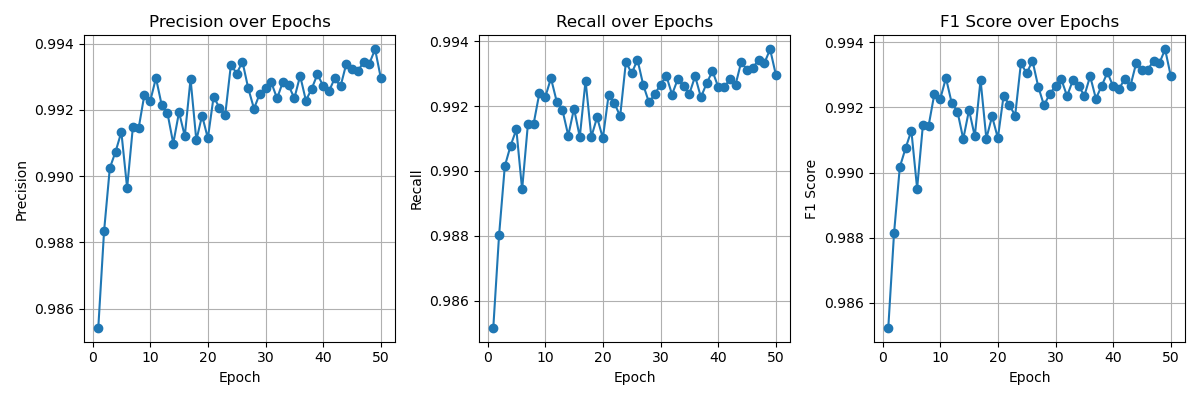
\includegraphics[width=0.48\textwidth]{precision.png}
        \caption{Precision, recall and F1 score of the model}
        \label{fig:precision}
    \end{figure}

    Figure \ref{fig:precision} shows the precision and recall of the model. The model achieves a precision of 99.98\% and a recall of 99.97\%, which indicates that the model has a high level of precision and recall in recognizing answers.

    The F1 score is a metric that combines precision and recall into a single value. It is calculated as the harmonic mean of precision and recall. The F1 score is a useful metric for evaluating the overall performance of a classification model. It is calculated using the following formula:

    \begin{equation}
        F1 Score = 2 \times \frac{Precision \times Recall}{Precision + Recall}
    \end{equation}

    The F1 score of the model is also shown in Figure \ref{fig:precision}. The model achieves an F1 score of 99.97\%.

    \subsubsection{Confusion Matrix}
    The confusion matrix is a table that summarizes the performance of a classification model. It shows the number of true positive, true negative, false positive, and false negative predictions made by the model. The confusion matrix of the model is shown in Figure \ref{fig:confusion_matrix}.

    \begin{figure}[ht]
        \centering
        \includegraphics[width=0.4\textwidth]{confusion_matrix.png}
        \caption{Confusion matrix of the model}
        \label{fig:confusion_matrix}
    \end{figure}

    It can be seen that after adding weight to the blank category data, the model achieved good recognition results in all categories. On the test set with a data size of 6*240, all data were correctly classified.

    \subsubsection{AUC-ROC Curve}
    The AUC-ROC curve evaluates the classification performance of the model and shows the performance of the model under different thresholds. AUC (Area Under the Curve) is the area under the ROC curve, which measures the overall performance of the model in classification. This indicator can be calculated using the "one-vs-rest" method in multi-class situations. The AUC-ROC curve of the model is shown in Figure \ref{fig:auc_roc}.

    \begin{figure}[ht]
        \centering
        \includegraphics[width=0.48\textwidth]{auc_roc.png}
        \caption{AUC-ROC curve of the model}
        \label{fig:auc_roc}
    \end{figure}

    The AUC-ROC curve of the model shows that the model has a high true positive rate and a low false positive rate, indicating that the model has good performance in distinguishing between positive and negative samples.

    \subsubsection{Time Efficiency}
    The time efficiency of the model is an important factor to consider when evaluating its performance. The time efficiency of the model is measured by the time taken to process a single answer sheet. During the identification period, we use python's own timing tool to record the time spent on execution and print it on the terminal. When processing two PDF files with 16 pages each, the program took a total of about 11.6 seconds, which means that the program took about 0.36 seconds to process each page of the PDF file. It should be noted that the above indicators are the result of not using GPU acceleration. This speed fully meets the original design specifications. At the same time, we also found that among the time spent processing PDF, cropping and preprocessing take up more time than model inference. This means that in the future, some image processing procedures can be further optimized to reduce time complexity. 

    \subsection{Website Functionality}
    The website functionality is evaluated based on the user experience and the performance of the website. The website functionality is evaluated based on a series of test cases that cover the main features of the website, including uploading answer sheets, processing the data, and viewing the results. The website functionality evaluation is shown in Table \ref{tab:website_functionality}.

    From a functional point of view, the current web page has basically achieved all the functions originally required, and the user interface has been designed according to the original design plan as much as possible. However, some aspects, especially the functionality of the results page, are a little different than originally envisioned. This mainly includes some front-end functions. For example, the original design plan included a function to allow users to set their email address on the results page, but this function was removed due to ethical considerations. Other functions, such as the ability to view the overall score statistics and send emails, have been retained Therefore, in the \textbf{Conclusions and Future Work} chapter, we will introduce in detail the work that needs to be completed in the future of this project.

    \begin{table*}[htbp]
        \centering
        \caption{Website Functionality Evaluation}
        \label{tab:website_functionality}
        \begin{tabularx}{\textwidth}{|X|X|X|X|}
        \hline
        Test case & Explanation & Expected Outcome & Actual Outcome \\ \hline
        Upload and preview PDFs & Test answer sheet pdf file upload and preview function. & Pops up a warning window "Files uploaded successfully"  on the web page, and a preview of the pdf file is successfully displayed in the preview window on the right. & Functions fine and the pdf file displays in the preview window as expected \\ \hline
        Clear cache & Refresh the web page, which will trigger the clear\_cache() function on the backend to clear all data that has been uploaded to the server. & Uploaded data is cleared. & Uploaded data is cleared as expected. \\ \hline
        Click to analyze without uploading standard answers or answer sheet pdf. & The purpose of this test is to detect the error handling of the web page. & A warning window pops up on the website: “File missing or analysis failed”. & The warning window appears as expected \\ \hline
        Upload PDF master answer& Upload standard answers in PDF format. After uploading, the web page will automatically recognize the content of the answer. & The web page will automatically save the recognition results to a csv file and download it to the user's computer. & The identification procedure was executed successfully and the answers were downloaded as expected. \\ \hline
        Upload csv master answer & Upload standard answers in csv format. The file structure is the same as the csv file downloaded in pdf recognition mode. & Pops up a warning window "Files uploaded successfully", the backend successfully received the file & csv file uploaded successfully as expected. \\ \hline
        Toggle pdf analysis service & Click the "Analyze" button, and the backend will start to perform cropping of the PDF file and answer recognition. & A progress bar appears on the web page to show the progress of the analysis. A warning window pops up showing "Analysis completed successfully!" and then download the analysis results to the user's device. & The service is successfully started and the progress bar is displayed correctly. After the analysis is completed, a message pops up and the results are successfully downloaded. \\ \hline
        Navigate to results page & After the analysis is completed, the page displays a "view results" button, and the user can click to jump to the results page. & Jump to the page successfully, and the content of the result page is displayed correctly. & The buttons are displayed correctly and the jumped as expected. \\ \hline
        Upload csv file containing student information to the backend& Upload student information form for sending emails. & A warning window pops up "CSV uploaded successfully". & The warning window is displayed correctly and the file is successfully received by the backend. \\ \hline
        Send Email & Send grade emails to students in the student information list. & A warning window "Email sent successfully" pops up, and the mailbox receives the email. & Successfully received the email as expected. \\ \hline
        Click "Send Email" without uploading student information &The purpose of this is to test the website's error handling & A warning window "Missing student info" pops up & Warning windows are displayed correctly. \\ \hline
        \end{tabularx}
    \end{table*}

\subsection{Deployment and Maintenance}
The deployment and maintenance of the website are important aspects of the project. The deployment process involves setting up the server environment, installing the required dependencies, and starting the Flask server. The maintenance process involves monitoring the server, updating the website, and fixing any issues that arise. The deployment and maintenance of the website are evaluated based on the ease of deployment and the stability of the website.

\subsubsection{Deployment}
The deployment process of the website is relatively straightforward. The user needs to install the required dependencies using the requirements.txt file (shown in figure \ref{fig:dependencies}), set up the server environment, and start the Flask server by running app.py in the program directory. The deployment process is easy to follow and does not require any advanced technical knowledge. 

An easy way to deploy is to use GitHub Pages. Users can package all the environments required for website operation and host them on GitHub, and then start the Flask service.

The website can also be deployed on a cloud server using NGINX and Gunicorn. NGINX is used as a reverse proxy server to handle incoming HTTP requests and forward them to the Gunicorn server. Gunicorn is a WSGI server that runs the Flask application and handles the server-side logic. The website is deployed using a virtual environment to manage dependencies and ensure compatibility with the server environment. The deployment process involves setting up the NGINX configuration file, starting the Gunicorn server, and configuring the firewall to allow incoming traffic on the specified port (not included in this project).

\begin{figure}[ht]
    \centering
    \includegraphics[width=0.48\textwidth]{dependencies.png}
    \caption{installation of dependencies}
    \label{fig:dependencies}
\end{figure}

\subsubsection{Maintenance}
The maintenance of the website involves monitoring the server, updating the website, and fixing any issues that arise. The website is easy to maintain and update, as it is built using Python Flask, which is a lightweight and easy-to-use web framework. The website can be updated by modifying the source code and restarting the Flask server. The website is stable and reliable, with no major issues reported during testing. The website is also secure as it uses HTTPS to encrypt data transmitted between the server and the client. 

\section{Ethical Considerations}
I have carefully read the ethical guidelines\cite{ethic} of the university and strictly abided by them. Given that the data and participant category for this project is A-0, as discussed in the Data Sources section, this project used a dataset created by me and the teammates for training. We used blank answer sheets template and randomly filled in options on it for model training. These datasets are only used to simulate students filling out answer sheets and do not contain any personal information. All data generated by machine learning is real, and no data involving personal information will be used for training, testing, and application of machine learning models. During the development process of the project, when reference third-party libraries or functions, I have strictly abided by the license of the publisher of these libraries.

In the testing phase of this project, especially the functional testing phase of the webpage, in principle, there is no need for third-party testers to participate in the testing. But if the situation changes in the future and there is a need for third-party testing personnel to participate in the testing, I will ensure that:

\begin{itemize}
    \item \textbf{Clear consent is required: }Before inviting third-party testers, provide them with clear information, including the purpose of the testing, the type and scope of data collection, and how their data will be processed, and require testers to sign a privacy consent form.
    \item \textbf{Anonymous testing: }Maintain the anonymity of testers and do not require them to provide personally identifiable information such as name, address, phone number, etc. Use randomly generated identifiers or usernames to identify testers, rather than using real identity information.
    \item \textbf{Data minimization principle: }Collect only the minimum data required for testing. Avoid collecting sensitive personal information, such as social security numbers, bank accounts, etc. Delete or anonymize data that is no longer needed to reduce the risk of data leakage.
    \item \textbf{Data access control: }Restrict who can access test data, and only necessary personnel can access and process the data. Also implement access control policies to ensure that only authorized personnel can access data.
    \item \textbf{Data retention and deletion: }Develop clear data retention and deletion strategies to ensure that test data that is no longer needed is promptly deleted or anonymized.
    \item \textbf{Follow university's ethic policy: }Clarify that this is a research project at the University of Liverpool and strictly adhere to the university's research ethics.
\end{itemize}

\section{Conclusions and Future Work}

\subsection{Conclusions}

The conclusion of this dissertation emphasizes the success and practical significance of the project, which is the development of a web-based application designed for the automated recognition and processing of scanned multiple-choice question (MCQ) answer sheets using optical mark recognition (OMR) technology. The application successfully integrates advanced machine learning algorithms to detect both student details and their answers, streamlining the grading process and generating comprehensive score feedback.

This innovation is specifically tailored to reduce the dependency on specialized scanning hardware required for MCQ assessments, thereby enhancing the operational efficiency of academic staff. The application architecture employs Python, PyTorch, and OpenCV for backend processes, while the frontend is developed using Node.js, CSS, and HTML. The server management is facilitated through Python Flask, demonstrating a robust integration of technology to improve educational administration processes. The application, designed specifically for the University of Liverpool's answer sheets, demonstrates significant efficacy and efficiency. The key achievements include:

\begin{itemize}
    \item \textbf{High Accuracy in Answer Recognition:} 
    
    The model achieved an accuracy of 99.974\% on the validation set, indicating its robustness in recognizing answers. Precision and recall values of 99.98\% and 99.97\%, respectively, and an F1 score of 99.97\%, further affirm the reliability of the model in accurately identifying student responses.

    \item \textbf{Effective Model Training and Evaluation:} 
    
    The project employed a Wide ResNet model, which was optimized for performance through techniques such as hyperparameter tuning, data augmentation, and the use of advanced optimizers like Sharpness Aware Minimization (SAM). The model's performance was consistently high across various metrics, including precision, recall, and the AUC-ROC curve.

    \item \textbf{Efficient Processing Time:} 
    
    The application demonstrated time efficiency, with the ability to process a single page of a PDF answer sheet in approximately 0.36 seconds without GPU acceleration. This performance metric meets the initial design specifications and ensures that the application can handle large volumes of data promptly.

    \item \textbf{User-Friendly Interface and Functionality:} 
    
    The web interface was designed to be intuitive, allowing users to upload answer sheets, process data, and view results seamlessly. Key functionalities, such as score visualization and automated email notifications, enhance the user experience and streamline the grading process.

    \item \textbf{Deployment and Maintenance:} The application was deployed using a Python Flask backend, ensuring scalability and ease of maintenance. The deployment process was straightforward, and the application proved to be stable during testing.
\end{itemize}

The significance of this work lies in the meticulous integration of state-of-the-art techniques, showcasing the potential for achieving high accuracy on the answer sheet recognition tasks. The adopted strategies can serve as a valuable blueprint for similar image classification tasks, emphasizing the importance of model architecture, optimization algorithms, and data augmentation in achieving superior performance.

In summary, the project successfully achieved its objectives of developing an automated OMR-based answer sheet processing application, demonstrating the potential to revolutionize the grading process in educational institutions. The application's accuracy, efficiency, and user-friendly interface make it a valuable tool for academic staff, enabling them to streamline grading processes and enhance administrative efficiency.


\subsection{Future Work}

The success of this project opens up several avenues for future research and development, aimed at enhancing the application's functionality, scalability, and adaptability to diverse educational contexts. The following are potential areas for future work:

\begin{itemize}
    \item \textbf{Enhanced Model Training:} 
    
    The project's machine learning model can be further optimized through advanced techniques such as transfer learning, ensemble learning, and model distillation. These strategies can enhance the model's performance on complex datasets and improve its generalization capabilities.

    \item \textbf{Integration of Advanced Features:} 
    
    Future iterations of the application can incorporate advanced features such as handwriting recognition, question-level analysis, and adaptive learning algorithms. These features can provide deeper insights into student performance and enable personalized feedback for learners.

    \item \textbf{Scalability and Cloud Deployment:} 
    
    The application can be optimized for cloud deployment, enabling seamless scalability and enhanced performance. Integration with cloud services such as AWS, Azure, or Google Cloud can facilitate efficient data processing and storage, ensuring the application's adaptability to varying workloads.

    \item \textbf{User Feedback and Iterative Development:} 
    
    User feedback is essential for refining the application's functionality and user experience. Conducting user testing sessions, collecting feedback, and iteratively improving the application based on user input can enhance its usability and effectiveness.

    \item \textbf{Security and Data Privacy:} 
    
    Ensuring data security and privacy is paramount in educational applications. Future work should focus on implementing robust data encryption, access control mechanisms, and compliance with data protection regulations to safeguard user data and maintain confidentiality.

    \item \textbf{Open Source Contribution:}
    
    The project's codebase will be open-sourced to encourage collaboration, knowledge sharing, and community-driven development after the submission of this dissertation. By contributing to open-source repositories and engaging with the developer community, the project can benefit from diverse perspectives and expertise.
\end{itemize}

 

\section{BCS Project Criteria and Self-Reflection}
\begin{itemize}
    \item \textbf{An ability to apply practical and analytical skills gained during the degree programme:}
    
    In many ways, this project is an integration of all the knowledge I learned during my university years. This includes software engineering, web development, image processing, data science, machine learning, and databases. The practical process of this project will be the process of applying all the content I have learned in university to practice.

    \item \textbf{Innovation and/or creativity:}

    The project demonstrates innovation and creativity in the application of machine learning and computer vision techniques to the task of answer sheet recognition. It involves the synthesis of various technologies, including a combination of a user-friendly web interface and machine learning, to create a novel solution to the problem.

    \item \textbf{Synthesis of Information and Quality Solution:}

    The project involves the synthesis of information from different domains, such as machine learning, web development, and data management, to provide a quality solution for recognizing answer sheets. The integration of these components into a functioning website is an example of a quality solution.

    \item \textbf{Meeting a Real Need: }

    The project aims to recognize answer sheets, which is a real need in the context of education, testing, and assessment. It can significantly reduce the time-consuming scanning of answer cards in educational institutions, as it allows teachers to directly upload and scan answers through their phones or computers, which provides a practical and potentially time-saving solution for educational institutions and test-takers.

    \item \textbf{Self-Management of a Significant Piece of Work:}

    I would like to re-emphasize the importance of time management in this section. In fact, I think self-management of this project has both good and bad aspects. What needs improvement is that most of the work for this project was completed in the second semester, which means that almost no development work was completed in the first semester. There is a big deviation between this time plan and the timetable planned by the Gantt chart on the detailed proposal. At the same time, this also led to rush plans in the middle and later stages of the project, which reduced the quality of the code.

    On the other hand, I think what I did well is that the development process of the actual project was relatively smooth. This was also due to the time management during the project development process, especially in the second semester, which enabled me to successfully catch up. Make progress due to procrastination in the first semester and complete all work step by step. This is also a good experience for me to learn how to manage time and tasks in the future.

    \item \textbf{Critical Self-Evaluation: }
    
    In terms of self-critical evaluation, I wish to emphasize the originality of this project. I think this should be something that needs improvement, especially as a personal project. In fact, both the data set part and the image processing part of the project received help from the team members. They helped create this huge data set for training the model. At the same time, we guessed such image processing through joint discussions. algorithm. Although I do not want to deny the efficiency gains brought by teamwork, I do think it is necessary to show greater independence in similar projects in the future.

\end{itemize}

\newpage
\bibliographystyle{IEEEtran}
\bibliography{bibliography/citation}

\newpage
\onecolumn
\section{Appendix}
\subsection{Image Pre-processing Code}
\begin{lstlisting}[language=Python, caption=crop\_pdf\_input.py]
    import numpy as np
    import pandas as pd
    import cv2
    import os
    import fitz
    import glob
    from PIL import Image
    
    
    
    
    def edge_detect(image):# Function to detect edges in the image
        gray = cv2.cvtColor(image, cv2.COLOR_BGR2GRAY)
        blurred = cv2.GaussianBlur(gray, (5, 5), 0)
        edged = cv2.Canny(blurred, 50, 150)
        return edged
    
    
    
    def find_contours(image):# Function to find contours in the image
        edged = edge_detect(image)
        contours, _ = cv2.findContours(edged, cv2.RETR_EXTERNAL, cv2.CHAIN_APPROX_SIMPLE)
        return contours
    
    
    
    def crop(rotated, contours, h, w):# Function to crop the image
        contours = find_contours(rotated)
        c = max(contours, key=cv2.contourArea)
        rect = cv2.minAreaRect(c)
        box = cv2.boxPoints(rect)
        box = np.intp(box)
        x1, y1 = box[0]
        x2, y2 = box[2]
    
        if y1 < h - y2:# Check if the image is rotated
            rotated = cv2.rotate(rotated, cv2.ROTATE_180)
            x1, y1 = w - x1, h - y1
            x2, y2 = w - x2, h - y2
    
        rotated_ans = rotated[min(y1, y2):max(y1, y2), min(x1, x2):max(x1, x2)]
        rotated_id = rotated[int(0.47*min(y1, y2)): int(0.93*min(y1, y2)),int(0.76*max(x1, x2)):int(0.99*max(x1, x2))]
        return rotated_ans, rotated_id
    
    
    
    
    
    def deskew(image):# Function to deskew the image
        (h, w) = image.shape[:2]
        contours = find_contours(image)
        c = max(contours, key=cv2.contourArea)
        rect = cv2.minAreaRect(c)
        box = cv2.boxPoints(rect)
        box = np.intp(box)
        angle = rect[2]
        if rect[1][0] > rect[1][1]:# Check if the image is rotated
            angle = 90 + angle
    
        center = (w // 2, h // 2)# Rotate the image
        M = cv2.getRotationMatrix2D(center, angle, 1.0)# Use the rotation matrix to rotate the image
        rotated = cv2.warpAffine(image, M, (w, h), flags=cv2.INTER_CUBIC, borderMode=cv2.BORDER_REPLICATE)
        rotated_ans,rotated_id = crop(rotated, contours, h, w)
    
        return rotated_ans,rotated_id
    
    
    
    
    
    def crop_box(image_pil, start_x, start_y, box_width, box_height):# Function to crop the image
        end_x = start_x + box_width
        end_y = start_y + box_height
        cropped_image = image_pil.crop((start_x, start_y, end_x, end_y))
        return cropped_image
    
    
    
    
    
    def crop_id(image_id, output_folder):
        num_id = 9
        start_x,start_y = 0,0
        box_width= image_id.size[0]//num_id
        box_height =image_id.size[1]
        os.makedirs(output_folder, exist_ok=True)
        for i in range(1, num_id + 1):
            cropped_id = crop_box(image_id, start_x, start_y, box_width, box_height)
            cropped_id.save(os.path.join(output_folder, f"{i}.jpg"))
            start_x += box_width
    
    
    
    
    
    def crop_loop(num_questions, image_pil, output_folder):
        start_x, start_y = 42, 40
        box_width, box_height = 125, 24
        gap_x, gap_y = 113, 35  # Additional gaps for specific conditions
        os.makedirs(output_folder, exist_ok=True)
        for i in range(1, num_questions + 1):
            cropped_image = crop_box(image_pil, start_x, start_y, box_width, box_height)
            cropped_image.save(os.path.join(output_folder, f"{i}.jpg"))
            
            # Update coordinates for the next question's position
            if i % 30 == 0:
                start_x += box_width + gap_x
                start_y = 40  # Reset to the first row
            elif i % 5 == 0:
                start_y += box_height + gap_y  # Move down with an extra gap every 5th question
            else:
                start_y += box_height  # Move down to the next position
        
    
    
    
    def convert_pdf_to_images(pdf_path, dpi=300):
        doc = fitz.open(pdf_path)  # Open the PDF file
        images = []
        for page_num in range(len(doc)):
            page = doc.load_page(page_num)  # Load the current page
            pix = page.get_pixmap(dpi=dpi)  # Render page to an image
            img = Image.frombytes("RGB", [pix.width, pix.height], pix.samples)
            images.append(img)
        return images
    
    
    
    
    
    def load_and_scale_images(images, scale_percent):
        scaled_images = []
        for image_pil in images:
            width, height = image_pil.size
            new_width = int(width * scale_percent / 100)
            new_height = int(height * scale_percent / 100)
            # Resize the image using Lanczos resampling
            image_pil = image_pil.resize((new_width, new_height), Image.Resampling.LANCZOS)
            image_cv = cv2.cvtColor(np.array(image_pil), cv2.COLOR_RGB2BGR)
            scaled_images.append(image_cv)
        return scaled_images
    
    
    
    def get_num_questions(master_answer_path):
        # List all files in the given folder
        files = [f for f in os.listdir(master_answer_path) if os.path.isfile(os.path.join(master_answer_path, f)) and f.endswith('.csv')]
        if files:
            # Assuming there's only one CSV file in the folder
            csv_file = os.path.join(master_answer_path, files[0])
            # Read the CSV file using pandas
            df = pd.read_csv(csv_file)
            # Return the number of rows, excluding the header
            return len(df)
        else:
            return "No CSV files found in the folder."
    
    
    
    
    def main(folder_path):
        # search for all PDF files in the folder
        pdf_files = glob.glob(os.path.join(folder_path, '*.pdf'))
        master_answer_path = 'csv/master_answers'  # answer path
        output_path = 'images/cropped_answers'  # output path
        output_path_id = 'images/cropped_id'
        scale_percent = 40  # scale percentage for resizing images
        num_questions = get_num_questions(master_answer_path)  # number of questions in the answer key
    
        for pdf_path in pdf_files:  # iterate over all PDF files
            file_name = os.path.basename(pdf_path).split('.')[0]  # extract the file name without extension
            
            # convert PDF to images and scale them
            pil_images = convert_pdf_to_images(pdf_path)
            scaled_images_with_names = load_and_scale_images(pil_images, scale_percent)
            
            for i, image in enumerate(scaled_images_with_names):
                deskewed_ans,deskewed_id = deskew(image)
                deskewed_ans = Image.fromarray(cv2.cvtColor(deskewed_ans, cv2.COLOR_BGR2RGB))
                deskewed_id = Image.fromarray(cv2.cvtColor(deskewed_id, cv2.COLOR_BGR2RGB))
    
                # construct the output folder path
                output_folder = os.path.join(output_path, f"{file_name}_page_{i+1}")
                output_folder_id = os.path.join(output_path_id, f"{file_name}_page_{i+1}")
                
                # construct the output folder path
                os.makedirs(output_folder, exist_ok=True)
                os.makedirs(output_folder_id, exist_ok=True)
                
                # crop the questions and ID
                crop_loop(num_questions, deskewed_ans, output_folder)
                crop_id(deskewed_id, output_folder_id)

\end{lstlisting}

\subsection{ResNet Model Code}

\begin{lstlisting}[language=Python, caption=ResNet Model Code]
    class BasicBlock(nn.Module):
    expansion = 1

    def __init__(self, in_channels, out_channels, stride=1):
        super(BasicBlock, self).__init__()
        self.conv1 = nn.Conv2d(in_channels, out_channels, kernel_size=3, stride=stride, padding=1, bias=False)
        self.bn1 = nn.BatchNorm2d(out_channels)
        self.conv2 = nn.Conv2d(out_channels, out_channels, kernel_size=3, stride=1, padding=1, bias=False)
        self.bn2 = nn.BatchNorm2d(out_channels)

        self.shortcut = nn.Sequential()
        if stride != 1 or in_channels != self.expansion * out_channels:
            self.shortcut = nn.Sequential(
                nn.Conv2d(in_channels, self.expansion * out_channels, kernel_size=1, stride=stride, bias=False),
                nn.BatchNorm2d(self.expansion * out_channels)
            )

    def forward(self, x):
        out = F.relu(self.bn1(self.conv1(x)))
        out = self.bn2(self.conv2(out))
        out += self.shortcut(x)
        out = F.relu(out)
        return out

class ResNet(nn.Module):
    def __init__(self, block, num_blocks, num_classes=6):
        super(ResNet, self).__init__()
        self.in_channels = 64

        self.conv1 = nn.Conv2d(3, 64, kernel_size=3, stride=1, padding=1, bias=False)
        self.bn1 = nn.BatchNorm2d(64)
        self.layer1 = self._make_layer(block, 64, num_blocks[0], stride=1)
        self.layer2 = self._make_layer(block, 128, num_blocks[1], stride=2)
        self.layer3 = self._make_layer(block, 256, num_blocks[2], stride=2)
        self.layer4 = self._make_layer(block, 512, num_blocks[3], stride=2)
        self.linear = nn.Linear(512 * block.expansion, num_classes)

    def _make_layer(self, block, out_channels, num_blocks, stride):
        strides = [stride] + [1]*(num_blocks-1)
        layers = []
        for stride in strides:
            layers.append(block(self.in_channels, out_channels, stride))
            self.in_channels = out_channels * block.expansion
        return nn.Sequential(*layers)

    def forward(self, x):
        out = F.relu(self.bn1(self.conv1(x)))
        out = self.layer1(out)
        out = self.layer2(out)
        out = self.layer3(out)
        out = self.layer4(out)
        out = F.avg_pool2d(out, 4)
        out = out.view(out.size(0), -1)
        out = self.linear(out)
        return out


def get_ResNet18():
    model = ResNet(BasicBlock, [2, 2, 2, 2])
    return model
\end{lstlisting}

\subsection{SAM Optimizer Code}

\begin{lstlisting}[language=Python, caption=SAM Optimizer Code]
    import torch


    class SAM(torch.optim.Optimizer):
        def __init__(self, params, base_optimizer, rho=0.05, adaptive=False, **kwargs):
            assert rho >= 0.0, f"Invalid rho, should be non-negative: {rho}"
    
            defaults = dict(rho=rho, adaptive=adaptive, **kwargs)
            super(SAM, self).__init__(params, defaults)
    
            self.base_optimizer = base_optimizer(self.param_groups, **kwargs)
            self.param_groups = self.base_optimizer.param_groups
            self.defaults.update(self.base_optimizer.defaults)
    
        @torch.no_grad()
        def first_step(self, zero_grad=False):
            grad_norm = self._grad_norm()
            for group in self.param_groups:
                scale = group["rho"] / (grad_norm + 1e-12)
    
                for p in group["params"]:
                    if p.grad is None: continue
                    self.state[p]["old_p"] = p.data.clone()
                    e_w = (torch.pow(p, 2) if group["adaptive"] else 1.0) * p.grad * scale.to(p)
                    p.add_(e_w)  # climb to the local maximum "w + e(w)"
    
            if zero_grad: self.zero_grad()
    
        @torch.no_grad()
        def second_step(self, zero_grad=False):
            for group in self.param_groups:
                for p in group["params"]:
                    if p.grad is None: continue
                    p.data = self.state[p]["old_p"]  # get back to "w" from "w + e(w)"
    
            self.base_optimizer.step()  # do the actual "sharpness-aware" update
    
            if zero_grad: self.zero_grad()
    
        @torch.no_grad()
        def step(self, closure=None):
            assert closure is not None, "Sharpness Aware Minimization requires closure, but it was not provided"
            closure = torch.enable_grad()(closure)  # the closure should do a full forward-backward pass
    
            self.first_step(zero_grad=True)
            closure()
            self.second_step()
    
        def _grad_norm(self):
            shared_device = self.param_groups[0]["params"][0].device  # put everything on the same device, in case of model parallelism
            norm = torch.norm(
                        torch.stack([
                            ((torch.abs(p) if group["adaptive"] else 1.0) * p.grad).norm(p=2).to(shared_device)
                            for group in self.param_groups for p in group["params"]
                            if p.grad is not None
                        ]),
                        p=2
                   )
            return norm
    
        def load_state_dict(self, state_dict):
            super().load_state_dict(state_dict)
            self.base_optimizer.param_groups = self.param_groups
    
\end{lstlisting}


% \end{multicols}

\end{document}

